\date{}
\title{}
\date{}
\begin{document}
\begin{frame}
    \titlepage
\end{frame}



\makeatletter
\newenvironment<>{btHighlight}[1][]
{\begin{onlyenv}#2\begingroup\tikzset{bt@Highlight@par/.style={#1}}\begin{lrbox}{\@tempboxa}}
{\end{lrbox}\bt@HL@box[bt@Highlight@par]{\@tempboxa}\endgroup\end{onlyenv}}

\newcommand<>\btHL[1][]{%
  \only#2{\begin{btHighlight}[#1]\bgroup\aftergroup\bt@HL@endenv}%
}
\def\bt@HL@endenv{%
  \end{btHighlight}%   
  \egroup %
}
\tikzset{
    btHLbox/.style={
        fill=red!30,outer sep=0pt,inner xsep=1pt, inner ysep=0pt, rounded corners=3pt
    },
}
\newcommand{\bt@HL@box}[2][]{%
  \tikz[#1]{%
    \pgfpathrectangle{\pgfpoint{1pt}{0pt}}{\pgfpoint{\wd #2}{\ht #2}}%
    \pgfusepath{use as bounding box}%
    \node[text width={},draw=none,anchor=base west, btHLbox, minimum height=\ht\strutbox+1pt,#1]{\raisebox{1pt}{\strut}\strut\usebox{#2}};
  }%
}

\lst@CCPutMacro
    \lst@ProcessOther {"2A}{%
      \lst@ttfamily 
         {\raisebox{2pt}{*}}% used with ttfamily
         {\raisebox{2pt}{*}}}% used with other fonts
    \@empty\z@\@empty

\lstdefinelanguage
   [x8664gas]{Assembler}     % add a "x64" dialect of Assembler
   [x86masm]{Assembler} % based on the "x86masm" dialect
   % with these extra keywords:
   {morekeywords={CDQE,CQO,CMPSQ,CMPXCHG16B,JRCXZ,LODSQ,MOVSXD,%
                  POPFQ,PUSHFQ,SCASQ,STOSQ,IRETQ,RDTSCP,SWAPGS,.TEXT,.STRING,.ASCIZ,%
                  BEQ,LW,SW,LB,SB,ADDIU,J,BEQZ,BNEZ,BNE,%
                  MOVUPD,MULPD,MOVSD,MULSD,%
                  SHLADD,MOV,CMP.LT,TBIT.NZ,BR.RET.SPTK.MANY,%
                  ADDQ,POPQ,PUSHQ,RRMOVQ,MRMOVQ,RMMOVQ,IRMOVQ,%
                  <-,LL,SC,ADDI,ADDL,VMOVDQA,ADDQ,CMPL,JB,JBE,MOVL,CLTQ,
                  MOVW,PUSHW,MOV,ADD,SUB,INT,PUSH,MOV,ADD,REP,MOVSB,%
                  TESTQ,CMPQ,MOVL,MOVQ,ADDQ,JMPQ,XORQ,%
                  LEAQ,LEAL,LEA,RETQ,RET,POPL,POPW,PUSHL,PUSHW,%
                  LEAW,%
                  SUBQ,SYSCALL,.ASCII,CALLQ,MOVSLQ,JMP,ANDQ,SHRQ,MOVB,INCQ,TESTL,XORL,%
                  SHRL,LEAL,SARL,SUBL,IMULL,IMULQ,MOVDQU,PADDD,XORL,%
                  MOVZBL,MOVZB,SHRB,SRAL,SHRL,ANDL,%
                  CMOVNS,SRAL,SRAQ,MOVZBW,MOVZBQ,%
                  PADDW,PADDQ,MODUPS,MOVAPD,%
                  MOVL,RET,.GLOBL,%
                  },
    deletekeywords={eax,ebx,sp,si,cx,di,ds,cs,es,fs,dx,ax,bx,al,esi,ebp,ecx,rip,eip,edx,edi,rdi,esp},
    morecomment=[l]{\#},
    morecomment=[l]{\/\/},
    morecomment=[s]{/*}{*/},
    sensitive=false,
    keepspaces=true} % et

\lstalias[]{myasm}[x8664gas]{Assembler}

\lstdefinelanguage{JavaScript}{
  keywords={typeof, new, true, false, catch, function, return, null, catch, switch, var, if, in, while, do, else, case, break},
  ndkeywords={class, export, boolean, throw, implements, import, this},
  sensitive=false,
  comment=[l]{//},
  morecomment=[s]{/*}{*/},
  morestring=[b]',
  morestring=[b]"
}

\newcommand{\keywordstyle}{\sourcecodeprolight\bfseries\color{blue!30!black}}
\newcommand{\stringstyle}{\color{blue!20!black}\ttfamily}

\lstset{
    language=C,
    basicstyle=\sourcecodepro\EmptyMapping,
    escapechar=`,
    keywordstyle=\keywordstyle\EmptyMapping,
    identifierstyle=\sourcecodepro\EmptyMapping,
    numberstyle=\small\color{black!70},
    commentstyle=\color{red!60!black}\ttfamily\itshape,
    stringstyle=\color{blue!20!black}\ttfamily,
    ndkeywordstyle=\bfseries\color{blue!30!black},
    upquote=true,
}



\lstdefinestyle{medium}{
    basicstyle=\sourcecodepro\EmptyMapping\fontsize{12}{13}\selectfont,
    keywordstyle=\sourcecodepro\EmptyMapping\fontsize{12}{13}\selectfont\keywordstyle,
}

\lstdefinestyle{small}{
    basicstyle=\sourcecodepro\EmptyMapping\small,
    keywordstyle=\sourcecodepro\EmptyMapping\small\keywordstyle,
}

\lstdefinestyle{smaller}{
    basicstyle=\sourcecodepro\EmptyMapping\fontsize{11}{12}\selectfont,
    keywordstyle=\sourcecodepro\EmptyMapping\fontsize{11}{12}\selectfont\keywordstyle,
}


\lstdefinestyle{script}{
    basicstyle=\sourcecodepro\EmptyMapping\scriptsize,
    keywordstyle=\sourcecodepro\EmptyMapping\scriptsize\bfseries,
}



\usetikzlibrary{patterns}

\begin{frame}
\frametitle{last time}
\begin{itemize}
\item fork = copy current process
    \begin{itemize}
    \item original = parent; new = child
    \item returns twice (once in new process, once in old)
    \item return value tells you which process you're in
    \end{itemize}
\item exec = load new program in current process
\item waitpid = wait for child process
\item fork + exec pattern
\end{itemize}
\end{frame}


\begin{frame}<1>[label=posixProcessFunctions]{POSIX process management}
\begin{itemize}
\item essential operations
\vspace{.5cm}
\item process information: \myemph<2>{\texttt{getpid}}
\item process creation: \myemph<3>{\texttt{fork}}
\item running programs: \myemph<4>{\texttt{exec*}}
\begin{itemize}
\item {\fontsize{9}{10}\selectfont also \texttt{posix\_spawn} (not widely supported), \ldots}
\end{itemize}
\item waiting for processes to finish: \texttt{\myemph<5>{waitpid}} {\small (or \texttt{\myemph<5>{wait}})}
\item process destruction, `signaling': \texttt{exit}, \texttt{kill}
\end{itemize}
\end{frame}


\subsection{fork exercise}

\begin{frame}[fragile,label=forkQuestion]{a fork question}
\vspace{-.3cm}
\begin{lstlisting}[language=C++,style=size10]
int main() {
    pid_t pid = fork();
    if (pid == 0) {
        printf("In child\n");
    } else {
        printf("Child %d\n", pid);
    }
    printf("Done!\n");
}
\end{lstlisting}
\tikzmark{question start}\small Exercise: Suppose the pid of the parent process is \texttt{99} and child is \texttt{100}. Give \textbf{two} possible outputs. (Assume no crashes, etc.)
\begin{tikzpicture}[overlay,remember picture]
\coordinate (timeline start) at ([yshift=-2cm]pic cs:question start);
\tikzset{
    prog1/.style={draw,fill=cyan},
    prog2/.style={draw,fill=green},
    proglabel/.style={font=\tt\scriptsize},
    labelprog1/.style={execute at begin node={\strut parent}},
    labelprog2/.style={execute at begin node={\strut child}},
}
\iftoggle{heldback}{}{
\begin{visibleenv}<2>
\begin{scope}[shift={(timeline start)}]
\begin{scope}[xscale=1.5,yscale=0.9]
    % FIXME: more suggestive split
\foreach \s/\e/\p [count=\x] in {0/1.5/1,1.5/3/2,3/4.5/1,4.5/5.5/2,5.5/7/1}{
    \coordinate (s-\x) at (\s, 0);
    \coordinate (e-\x) at (\e, 0);
    \draw[prog\p] (\s, 0) rectangle (\e, 1) coordinate[midway] (mid-\x);
    \node[anchor=center,proglabel,labelprog\p] at (mid-\x) {};
    \draw[fill=white] ([xshift=-.05cm]e-\x) rectangle ([xshift=.05cm,yshift=1cm]e-\x);
    \draw[pattern=north west lines] ([xshift=-.05cm]e-\x) rectangle ([xshift=.05cm,yshift=1cm]e-\x);
}
\node[overlay,anchor=west,font=\tt\fontsize{9}{10}\selectfont,align=left] at (7.5, .8) { Child 100 \\ In child \\ Done! \\ Done!};
\begin{scope}[yshift=-1.5cm]
\foreach \s/\e/\p [count=\x] in {0/1/1,1/4/2,4/7/1}{
    \coordinate (s-\x) at (\s, 0);
    \coordinate (e-\x) at (\e, 0);
    \draw[prog\p] (\s, 0) rectangle (\e, 1) coordinate[midway] (mid-\x);
    \node[anchor=center,proglabel,labelprog\p] at (mid-\x) {};
    \draw[fill=white] ([xshift=-.05cm]e-\x) rectangle ([xshift=.05cm,yshift=1cm]e-\x);
    \draw[pattern=north west lines] ([xshift=-.05cm]e-\x) rectangle ([xshift=.05cm,yshift=1cm]e-\x);
}
\node[anchor=west,font=\tt\fontsize{9}{10}\selectfont,align=left] at (7.5, .5) { In child \\ Done! \\ Child 100 \\ Done! };
\end{scope}
\end{scope}
\end{scope}
\end{visibleenv}
}
\end{tikzpicture}
\end{frame}



\begin{frame}[fragile,label=forkQuestion]{a fork question (2)}
\vspace{-.3cm}
\begin{lstlisting}[language=C++,style=size10]
int x = 0;
int main() {
    pid_t pid = fork();
    int y = 0;
    if (pid == 0) {
        x += 1;
        y += 2;
    } else {
        x += 3;
        y += 4;
    }
    printf("%d %d\n", x, y);
}
\end{lstlisting}
\tikzmark{question start}\small Exercise: which (possibly multiple) are possible outputs?
\begin{tabular}{lll}
A. 1 2 (newline) 3 4 &
B. 1 2 (newline) 4 4 &
C. 1 2 (newline) 4 6 \\
D. 3 4 (newline) 1 2 &
E. 3 4 (newline) 4 6 &
F. 4 6 (newline) 4 6 \\
\end{tabular}
\end{frame}


\subsection{exec}

\againframe<4>{posixProcessFunctions}

\usetikzlibrary{matrix,patterns,arrows.meta,decorations.pathreplacing,shapes.misc,fit}

\begin{frame}{exec*}
\begin{itemize}
\item exec* --- \myemph{replace} current program with new program
    \begin{itemize}
    \item * --- multiple variants
    \item same pid, new process image
    \end{itemize}
\item \texttt{int execv(const char *path, const char **argv)}
    \begin{itemize}
    \item path: new program to run
    \item argv: array of arguments, termianted by null pointer
    \end{itemize}
\end{itemize}
\end{frame}

\begin{frame}[fragile,label=execExample1]{execv example}
\begin{lstlisting}[
    language=C++,
    style=small,
    moredelim={**[is][\btHL<2|handout:0>]{@2}{2@}},
    moredelim={**[is][\btHL<3|handout:0>]{@3}{3@}},
    moredelim={**[is][\btHL<4|handout:0>]{@4}{4@}},
]
  ...
  child_pid = fork();
  if (child_pid == 0) {
    /* child process */
    char *args[] = @2{"ls", "-l", NULL}2@;
    execv(@3"/bin/ls"3@, @2args2@);
    /* execv doesn't return when it works.
       So, if we got here, it failed. */
    perror("execv");
    exit(1);
  } else if (child_pid > 0) {
    /* parent process */
    ...
  }
\end{lstlisting}
\begin{tikzpicture}[overlay,remember picture]
\coordinate (explain location) at ([xshift=-1cm,yshift=-5cm]current page.north east);
\tikzset{
    explain box/.style={
        at={(explain location)},
        anchor=north east,
        draw=red,
        very thick,
        align=left,
        fill=white
    },
}
\begin{visibleenv}<2|handout:0>
\node[explain box] {
used to compute argv, argc \\
when program's \texttt{main} is run \\
~ \\
convention: first argument is program name
};
\end{visibleenv}
\begin{visibleenv}<3|handout:0>
\node[explain box] {
path of executable to run \\
need not match first argument \\
(but probably should match it) \\
~  \\
on Unix {\texttt /bin} is a directory \\
containing many common programs, \\
including \texttt{ls} (`list directory')
};
\end{visibleenv}
\end{tikzpicture}
\end{frame}


\usetikzlibrary{fit,arrows.meta,matrix,decorations.pathreplacing,shapes.misc}

\begin{frame}{exec in the kernel}
\begin{tikzpicture}
\tikzset{
    pcb/.style={
        tight matrix,
        column 1/.style={nodes={draw,thin,text width=3cm,font=\small,minimum height=0.4cm}},
        column 2/.style={nodes={draw,thin,text width=4cm,font=\fontsize{9}{10}\tt\selectfont,minimum height=0.4cm}},
    },
    page/.style={
        draw,thick,
        pattern=north west lines,
        minimum width=2cm,
        node contents={~},
    },
    pointer/.style={
        draw,very thick,-Latex,
    },
    pointer light/.style={
        draw,thick,-Latex,
    },
    tall/.style={
        minimum height=0.85cm
    },
    one pt/.style={
        fill=blue!40,
    },
    one pt line/.style={
        draw=blue!80!black,
    },
    one memory/.style={
        fill=green!40,
    },
    one memory line/.style={
        draw=green!80!black,
        alt=<2->{opacity=0.2,dotted},
    },
    two memory/.style={
        fill=violet!40,
        alt=<2>{draw=red,thick},
    },
    two memory line/.style={
        draw=violet!80!black,
    },
    mark line/.style={
        draw,thick,Latex-,
    },
    mark line reversed/.style={
        draw,thick,-Latex,
    }
}
\matrix[pcb,label={[font=\small]north:the process control block}] (proc one) {
    |[tall]| user regs \&
    |[tall]|
    {eax=\sout<2->{42}{\normalfont\it \only<2->{\myemph<2>{init. val.}}}, \\ ecx=\sout<2->{133}\only<2->{\normalfont\it \myemph<2>{init. val.}},} \ldots \\
    memory mapping\& |[one pt]| ~ \\
    |[tall]| open files \& |[tall,alt=<4>{red,thick},alias=fds]| {fd 0: (terminal \ldots) \\ fd 1: \ldots } \\
    \ldots \& \ldots \\
};
\newcommand{\halfvthick}{.2mm}
\node[draw,very thick,pattern=north west lines,minimum width=2cm,minimum height=6cm,anchor=north west,
    label={north:memory}] (memory) at ([xshift=3cm,yshift=0cm]proc one.north east) {};
\draw[pointer,one pt line] (proc one-2-2.east) -- ++(.5cm,0cm) |- ([yshift=-1.8cm]memory.north west) coordinate (one pt base);
\foreach \y in {-1.8cm} {
    \draw[very thick,one pt] ([yshift=\y,xshift=\halfvthick]memory.north west) rectangle ++ (2cm,-1mm);
}
\draw[pointer light,one memory line] ([yshift=-.2mm]one pt base) -- ++(-.5cm,0cm) |- ([yshift=-0.9cm]memory.north west);
\draw[pointer light,one memory line] ([yshift=-.1mm]one pt base) -- ++(-.6cm,0cm) |- ([yshift=-1.1cm]memory.north west) coordinate (args memory);
\draw[pointer light,one memory line] ([yshift=.1mm]one pt base) -- ++(-.7cm,0cm) |- ([yshift=-1.5cm]memory.north west);
\foreach \y/\v in {-0.9cm/A,-1.1cm/B,-1.5cm/C} {
    \draw[very thick,one memory] ([yshift=\y,xshift=\halfvthick]memory.north west) coordinate (orig-\v) rectangle ++ (2cm,-1mm) coordinate (orig-other-\v);
}
\begin{visibleenv}<2->
\draw[pointer light,two memory line] ([yshift=-.1mm]one pt base) -- ++(-.5cm,0cm) |- ([yshift=-4.4cm]memory.north west);
\draw[pointer light,two memory line] ([yshift=-.2mm]one pt base) -- ++(-.6cm,0cm) |- ([yshift=-4.6cm]memory.north west);
\draw[pointer light,two memory line] ([yshift=-.3mm]one pt base) -- ++(-.7cm,0cm) |- ([yshift=-5cm]memory.north west);
\draw[pointer light,two memory line] ([yshift=-.4mm]one pt base) -- ++(-.8cm,0cm) |- ([yshift=-5.1cm]memory.north west);
\foreach \y in {-4.4cm,-4.6cm,-5cm,-5.1cm} {
    \draw[very thick,two memory] ([yshift=\y,xshift=\halfvthick]memory.north west) rectangle ++ (2cm,-1mm);
}
\draw[mark line] ([yshift=-5.15cm]memory.north east) -| ++(2cm,-.5cm) node[below,align=center,font=\small] { \myemph<2>{loaded from} \\ \myemph<2>{executable file} };
\coordinate (new memory) at ([yshift=-4.7cm,xshift=.25cm]memory.north east);
\draw[ultra thick,decorate,decoration={brace,mirror}] ([xshift=-.15cm,yshift=-3mm]new memory) -- ([xshift=-.15cm,yshift=3mm]new memory);
\node[anchor=west,font=\small] (new stack text) at ([xshift=-1.5mm]new memory) { \myemph<2>{new stack, heap, \ldots} };
\end{visibleenv}
\begin{visibleenv}<3->
\draw[mark line reversed] ([xshift=2cm]args memory) -| (new stack text.north) node[pos=0.75,fill=white,font=\small] {\myemph<3>{copy arguments}};
\end{visibleenv}
\begin{visibleenv}<4->
    \draw[mark line,alt=<4>{draw=red}{blue},ultra thick] (fds.south) -- ++(0cm, -2cm) node[below,align=center] { files + some other things not changed! \\ (more on this later) };
\end{visibleenv}
\begin{visibleenv}<5>
\node[cross out,draw=red,very thick,fit=(orig-A) (orig-other-C),label={[align=center,red]north east:old memory\\discarded}] {};
\end{visibleenv}
\end{tikzpicture}
\end{frame}


\subsection{aside: fork+exec, really?}

\begin{frame}{why fork/exec?}
    \begin{itemize}
    \item could just have a function to spawn a new program
        \begin{itemize}
        \item Windows \texttt{CreateProcess()}; POSIX's (rarely used) \texttt{posix\_spawn}
        \end{itemize}
    \vspace{.5cm}
    \item some other OSs do this (e.g. Windows)
    \item needs to include API to set new program's state
        \begin{itemize}
        \item e.g. without fork: either: \\
        need function to set new program's current directory, \textit{or} \\
        need to change your directory, then start program, then change back
        \item e.g. with fork: just change your current directory before exec
        \end{itemize}
    \item but allows OS to avoid `copy everything' code
        \begin{itemize}
        \item probably makes OS implementation easier
        \end{itemize}
    \end{itemize}
\end{frame}

\begin{frame}[fragile,label=posixSpawn]{posix\_spawn}
\begin{lstlisting}[style=small]
pid_t new_pid;
const char argv[] = { "ls", "-l", NULL };
int error_code = posix_spawn(
    &new_pid,
    "/bin/ls",
    NULL /* null = copy current process's open files;
            if not null, do something else */,
    NULL /* null = no special settings for new process */,
    argv,
    NULL /* null = copy current "environment variables", 
            if not null, do something else */
);
if (error_code == 0) {
    /* handle error */
}
\end{lstlisting}
\end{frame}

\begin{frame}{some opinions (via HotOS '19)}

\includegraphics[width=5in]{../unix-api/fork-in-road-title}
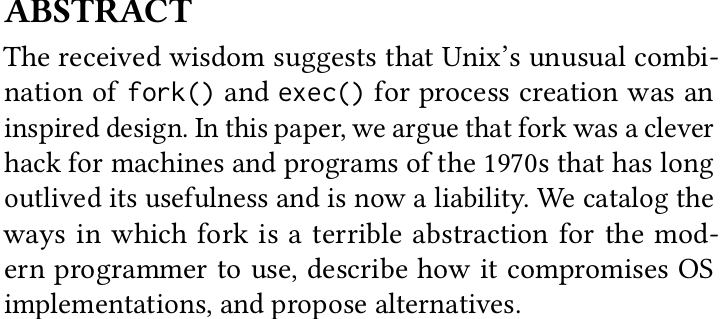
\includegraphics[width=5in]{../unix-api/fork-in-road-abs}
\end{frame}


\subsection{wait}

\againframe<5>{posixProcessFunctions}

\begin{frame}{wait/waitpid}
\begin{itemize}
\item \texttt{pid\_t waitpid(pid\_t pid, int *status, \\
              \hspace{5cm} int options)}
\item wait for a child process (with pid=\texttt{pid}) to finish
\item sets \texttt{*status} to its ``status information''
\vspace{.5cm}
\item \texttt{pid=-1} $\rightarrow$ wait for any child process instead
    \begin{itemize}
    \item \texttt{pid=0} almost the same
    \end{itemize}
\item options? see manual page (command \texttt{man waitpid})
    \begin{itemize}
        \item \texttt{0} --- no options
        %\item \myemph<2>{\texttt{WNOHANG}} --- return 0 rather than hanging if process not yet done
    \end{itemize}
\end{itemize}
\end{frame}

\begin{frame}[fragile,label=waitpidExample]{waitpid example}
\begin{lstlisting}[
    language=C++,
    style=smaller
]
#include <sys/wait.h>
...
  child_pid = fork();
  if (child_pid > 0) {
      /* Parent process */
      int status;
      waitpid(child_pid, &status, 0);
  } else if (child_pid == 0) {
      /* Child process */
      ...
\end{lstlisting}
\end{frame}



\begin{frame}[fragile,label=exitStatuses]{exit statuses}
\begin{lstlisting}[
    language=C++,
    moredelim={**[is][\btHL<1-|handout:1->]{@1}{1@}},
]
int main() {
    return @101@;  /* or exit(0);  */
}
\end{lstlisting}
\end{frame}

\begin{frame}[fragile,label=extractStatus]{the status}
\begin{lstlisting}[
    language=C++,
    style=smaller,
    moredelim={**[is][\btHL<2|handout:0>]{@2}{2@}},
]
#include <sys/wait.h>
...
  waitpid(child_pid, &status, 0);
  if (@2WIFEXITED(status)2@) {
    printf("main returned or exit called with %d\n",
           @2WEXITSTATUS(status)2@);
  } else if (WIFSIGNALED(status)) {
    printf("killed by signal %d\n", WTERMSIG(status));
  } else {
      ...
  }
\end{lstlisting}
``status code'' encodes \myemph{both return value and if exit was abnormal} \\
W* macros to decode it
\end{frame}


\subsection{summary diagram}

\usetikzlibrary{arrows.meta,decorations.pathmorphing,fadings}

\begin{frame}[fragile,label=typicalPatternSnake]{typical pattern}
\begin{tikzpicture}
\tikzset{
    thread/.style={very thick,draw,decorate,decoration=snake},
    split/.style={very thick,draw},
    marker/.style={thin,draw},
}
\path[thread] (0, 0) --  (0, -.5);
\node[anchor=south] at (0,0) {parent};
\node[anchor=north] (fork mark) at (0, -.5) {fork};
\draw[thread] (fork mark.south) -- (0, -2) node[below] (wait start) {waitpid};
\node (child start) at (9, -1.5) {child process};
\path[split] (fork mark) --  (child start);
\path[thread] (child start.south) -- (9, -2.5) node[below] (exec) {exec};
\path[thread] (exec.south) -- ++(0, -2) coordinate (exec done);
\path[marker] (exec done) -- ++(.5, 0) node[right] {exit()};
\path[split,dotted] (exec done) -- (0, -6);
\draw[very thick,dashed] (wait start) -- (0, -6);
\path[thread] (0, -6) -- ++(0, -3);
\end{tikzpicture}
\end{frame}


\begin{frame}[fragile,label=typicalPatternSnakeAlt]{typical pattern (alt)}
\begin{tikzpicture}
\tikzset{
    thread/.style={very thick,draw,decorate,decoration=snake},
    split/.style={very thick,draw},
    marker/.style={thin,draw},
}
\path[thread] (0, 0) --  (0, -.5);
\node[anchor=south] at (0,0) {parent};
\node[anchor=north] (fork mark) at (0, -.5) {fork};
\draw[thread] (fork mark.south) -- (0, -5.5) node[below] (wait start) {waitpid};
\node (child start) at (9, -1.5) {child process};
\path[split] (fork mark) --  (child start);
\path[thread] (child start.south) -- (9, -2.5) node[below] (exec) {exec};
\path[thread] (exec.south) -- ++(0, -1) coordinate (exec done);
\path[marker] (exec done) -- ++(.5, 0) node[right] {exit()};
\path[split,dotted] (exec done) -- (wait start.east);
%\draw[very thick,dashed] (wait start) -- (0, -6);
\path[thread] (wait start.south) -- ++(0, -3);
\end{tikzpicture}
\end{frame}

\begin{frame}[fragile,label=typicalPattern]{typical pattern (detail)}
\newcommand{\maincode}{
            pid = fork(); \\
            if (pid == 0) \{ \\
            \hspace{.5cm} exec\ldots(\ldots); \\
            \hspace{.5cm} \ldots \\
            \} else if (pid > 0) \{ \\
            \hspace{.5cm} waitpid(pid,\ldots); \\
            \hspace{.5cm} \ldots \\
            \} \\
            \ldots
}
\newcommand{\maincodeExec}{
            pid = fork(); \\
            if (pid == 0) \{ \\
            \hspace{.5cm} \myemph{exec\ldots(\ldots);} \\
            \hspace{.5cm} \ldots \\
            \} else if (pid > 0) \{ \\
            \hspace{.5cm} waitpid(pid,\ldots); \\
            \hspace{.5cm} \ldots \\
            \} \\
            \ldots
}
\newcommand{\maincodeWait}{
            pid = fork(); \\
            if (pid == 0) \{ \\
            \hspace{.5cm} exec\ldots(\ldots); \\
            \hspace{.5cm} \ldots \\
            \} else if (pid > 0) \{ \\
            \hspace{.5cm} \myemph{waitpid(pid,\ldots);} \\
            \hspace{.5cm} \ldots \\
            \} \\
            \ldots
}
\newcommand{\altcode}{
            main() \{ \\
            \hspace{.5cm} \ldots \\
            \} \\
}
\begin{tikzpicture}
\tikzset{
    code box/.style={draw,thick,font=\tt\fontsize{9}{10}\selectfont,align=left},
    with the code/.style={
        code box,
    },
    with the other code/.style={
        code box,
    }
}
\node[with the code] (start) {\maincode};
\node[with the code,anchor=north west] (parent first) at ([xshift=2cm,yshift=1cm]start.south east) {\maincodeWait};
\node[with the code,anchor=south west] (child first) at ([xshift=2cm,yshift=-1cm]start.north east) {\maincodeExec};
\node[with the other code,anchor=north west] (child second) at ([xshift=2cm]child first.north east) {\altcode};

\begin{scope}[very thick,>=Latex]
\draw[->] (start) -- (parent first);
\draw[->] (start) -- (child first);
\draw[->] (child first) -- (child second);
\end{scope}
\end{tikzpicture}
\end{frame}



\againframe<6>{posixProcessFunctions}

\subsection{exercises (fork+exec+wait)}

\begin{frame}[fragile,label=fork-wait-ex1]{exercise (1)}
\vspace{-.25cm}
\begin{lstlisting}[basicstyle=\fontsize{9.5}{10.5}\tt\selectfont]
int main() {
    pid_t pids[2]; const char *args[] = {"echo", "ARG", NULL};
    const char *extra[] = {"L1", "L2"};
    for (int i = 0; i < 2; ++i) {
        pids[i] = fork();
        if (pids[i] == 0) {
            args[1] = extra[i];
            execv("/bin/echo", args);
        }
    }
    for (int i = 0; i < 2; ++i) {
        waitpid(pids[i], NULL, 0);
    }
}
\end{lstlisting}
\newcommand{\shownewline}{ {\fontsize{9}{10}\selectfont(newline)} }
Assuming fork and execv do not fail, which are possible outputs?
\begin{tabular}{llll}
\bfseries A. & \tt L1\shownewline L2 & \bfseries D. & A and B \\
\bfseries B. & \tt L1\shownewline L2\shownewline L2 & \bfseries E. & A and C \\
\bfseries C. & \tt L2\shownewline L1 & \bfseries F. & all of the above \\
    ~ &  ~ & \bfseries G. & something else \\
\end{tabular}
\end{frame}

\iftoggle{heldback}{\providecommand{\correct}[1]{#1}}{\providecommand{\correct}[1]{\myemph<2>{#1}}}

\begin{frame}[fragile,label=fork-wait-ex2]{exercise (2)}
\vspace{-.4cm}
\begin{lstlisting}[basicstyle=\fontsize{9.5}{10.5}\tt\selectfont]
int main() {
    pid_t pids[2]; const char *args[] = {"echo", "0", NULL};
    for (int i = 0; i < 2; ++i) {
        pids[i] = fork();
        if (pids[i] == 0) { execv("/bin/echo", args); }
    }
    printf("1\n"); fflush(stdout);
    for (int i = 0; i < 2; ++i) {
        waitpid(pids[i], NULL, 0);
    }
    printf("2\n"); fflush(stdout);
}
\end{lstlisting}
\newcommand{\shownewline}{ {\normalfont\fontsize{9}{10}\selectfont(newline)} }
Assuming fork and execv do not fail, which are possible outputs?
\begin{tabular}{llll}
\bfseries A. & \tt 0\shownewline 0\shownewline 1\shownewline 2 & \bfseries E. & \correct{A, B, and C} \\
\bfseries B. & \tt 0\shownewline 1\shownewline 0\shownewline 2 & \bfseries F. & C and D \\
\bfseries C. & \tt 1\shownewline 0\shownewline 0\shownewline 2 & \bfseries G. & all of the above \\
\bfseries D. & \tt 1\shownewline 0\shownewline 2\shownewline 0 & \bfseries H. & something else \\
\end{tabular}
\end{frame}


\subsection{aside re: fork bombs}
\begin{FragileFrame}\frametitle{warning re: forking in loops}
\lstset{language=C,style=smaller}
\begin{lstlisting}
while (true) {
    fork();
}
\end{lstlisting}
    \begin{itemize}
    \item what's going to happen?
        \begin{itemize}
        \item lots of CPU being used
        \item lots of memory being allocated
        \item control-C might only terminate one of the processes
        \end{itemize}
    \item<2-> \myemph{probably very bad and hard to recover from}
    \end{itemize}
\end{FragileFrame}

\begin{frame}{some recommendations re: timing}
    \begin{itemize}
    \item in timing assignment, you'll need to run \texttt{fork()} multiple times to measure it
    \vspace{.5cm}
    \item I recommend:
    \item always waitpid \myemph{successfully} before fork()ing a second time
    \item test fork()ing exactly once before doing a loop
    \end{itemize}
\end{frame}


% FIXME: TODO: talk about kill() here

\section{shell features}
\begin{frame}<1>[fragile,label=commandLineFeatures]{some POSIX command-line features}
\begin{itemize}
\item \myemph<2>{searching for programs}
    \begin{itemize}
    \item \verb|ls -l| $\approx$ \verb|/bin/ls -l|
    \item \verb|make| $\approx$ \verb|/usr/bin/make|
    \end{itemize}
\item running in background
    \begin{itemize}
    \item \verb|./someprogram &|
    \end{itemize}
\item \myemph<4>{redirection}:
    \begin{itemize}
    \item \verb|./someprogram >output.txt|
    \item \verb|./someprogram <input.txt|
    \end{itemize}
\item \myemph<5>{pipelines}:
    \begin{itemize}
    \item \verb!./someprogram | ./somefilter!
    \end{itemize}
\end{itemize}
\end{frame}




\section{fd management}
\subsection{I/O redirection: syntax, method preview}

\againframe<4>{commandLineFeatures}


\section{files in POSIX, part 1}

\subsection{interlude: file descriptors}

\begin{frame}[fragile,label=fds]{file descriptors}
\begin{lstlisting}[language=C,style=smaller]
struct process_info {  /* <-- in the kernel somewhere */
    ...
    struct open_file_description *files[SIZE];
    ...
};
...
process->files[file_descriptor]
\end{lstlisting}
    \begin{itemize}
    \item Unix: every process has \\
        array (or similar) of \textit{open file descriptions}
    \item ``open file'': {\small terminal $\cdot$ socket $\cdot$ regular file $\cdot$ pipe}
    \item file descriptor = index into array
        \begin{itemize}
        \item usually what's used with system calls
        \item stdio.h FILE*s usually have file descriptor + buffer
        \end{itemize}
    \end{itemize}
\end{frame}






\begin{frame}{special file descriptors}
\begin{itemize}
\item file descriptor 0 = standard input
\item file descriptor 1 = standard output
\item file descriptor 2 = standard error
\vspace{.5cm}
\item constants in \texttt{unistd.h}
    \begin{itemize} \item \texttt{STDIN\_FILENO}, \texttt{STDOUT\_FILENO}, \texttt{STDERR\_FILENO} \end{itemize}
\vspace{.5cm}
\item<2-> but you can't choose which number \texttt{open} assigns\ldots?
    \begin{itemize}
    \item more on this later
    \end{itemize}
\end{itemize}
\end{frame}



\subsection{getting file descriptors}


\begin{frame}[fragile,label=gettingFds]{getting file descriptors}
\begin{lstlisting}[
    language=C++,
    moredelim={**[is][\btHL<1-|handout:1->]{@1}{1@}},
    style=smaller
]
int read_fd = open("dir/file1", O_RDONLY);
int write_fd = open("/other/file2", O_WRONLY | ...);
int rdwr_fd = open("file3", O_RDWR);
\end{lstlisting}
\begin{itemize}
\item used internally by fopen(), etc.
\item also for files without normal filenames\ldots:
\end{itemize}
\begin{lstlisting}[
    language=C++,
    moredelim={**[is][\btHL<1-|handout:1->]{@1}{1@}},
    style=smaller,
]
int fd = shm_open("/shared_memory", O_RDWR, 0666); // shared memory
int socket_fd = socket(AF_INET, SOCK_STREAM, 0); // TCP socket
int term_fd = posix_openpt(O_RDWR); // pseudo-terminal
int pipe_fds[2]; pipe(pipefds); // "pipes" (later)
...
\end{lstlisting}
\end{frame}

\begin{frame}[fragile,label=flagsExplain]{open: flags}
\begin{lstlisting}[
    language=C++,
    moredelim={**[is][\btHL<1-|handout:1->]{@1}{1@}},
]
int open(const char *path, int @1flags1@);
int open(const char *path, int @1flags1@, int mode);
\end{lstlisting}
\begin{itemize}
\item flags: bitwise or of:
    \begin{itemize}
    \item \texttt{O\_RDWR}, \texttt{O\_RDONLY}, or \texttt{O\_WRONLY}
        \begin{itemize}
        \item read/write, read-only, write-only
        \end{itemize}
    \item \texttt{O\_APPEND}
        \begin{itemize}
        \item append to end of file
        \end{itemize}
    \item \texttt{O\_TRUNC}
        \begin{itemize}
        \item truncate (set length to 0) file if it already exists
        \end{itemize}
    \item \texttt{O\_CREAT}
        \begin{itemize}
        \item create a new file if one doesn't exist
        \item (default: file must already exist)
        \end{itemize}
    \item \ldots and more % FIXME: O_EXCL omitted
    \end{itemize}
\item \texttt{man 2 open}
\end{itemize}
\end{frame}

\begin{frame}[fragile,label=modeExplain]{open: mode}
\begin{lstlisting}[
    language=C++,
    moredelim={**[is][\btHL<1-|handout:1->]{@1}{1@}},
]
int open(const char *path, int flags);
int open(const char *path, int flags, int @1mode1@);
\end{lstlisting}
\begin{itemize}
\item mode: permissions of newly created file
    \begin{itemize}
    \item like numbers provided to \texttt{chmod} command
    \item filtered by a ``umask''
    \end{itemize}
\item simple advice: always use \texttt{0666}
    \begin{itemize}
    \item = readable/writeable by everyone, except where umask prohibits
    \item (typical umask: prohibit other/group writing)
    \end{itemize}
\end{itemize}
\end{frame}


\subsection{close}

\begin{frame}[fragile,label=close]{close}
\begin{lstlisting}[language=C++]
int close(int fd);
\end{lstlisting}
\begin{itemize}
\item close the file descriptor, deallocating that array index
    \begin{itemize}
    \item does not affect other file descriptors \\ that refer to same ``open file description''
    \item (e.g. in \texttt{fork()}ed child or created via (later) \texttt{dup2})
    \end{itemize}
\item if last file descriptor for open file description, resources deallocated
\vspace{.5cm}
\item returns 0 on success
\item returns -1 on error
    \begin{itemize}
    \item e.g. ran out of disk space while finishing saving file
    \end{itemize}
\end{itemize}
\end{frame}


\subsection{Shell: redirection}

\usetikzlibrary{matrix,patterns,arrows.meta,decorations.pathreplacing,shapes.misc,fit}

\begin{frame}[fragile,label=redirectExample]{shell redirection}
\begin{itemize}
\item \verb|./my_program ... < input.txt|:
    \begin{itemize}
    \item run \verb|./my_program ...| but use \verb|input.txt| as input
    \item like we copied and pasted the file into the terminal
    \end{itemize}
\vspace{.5cm}
\item \verb|echo foo > output.txt|:
    \begin{itemize}
    \item runs \verb|echo foo|, sends output to \verb|output.txt|
    \item like we copied and pasted the output into that file
    \item (as it was written)
    \end{itemize}
\end{itemize}
\end{frame}

\begin{frame}[fragile,label=forkTrick]{fork copies open file list}
\begin{tikzpicture}
\tikzset{
    >=Latex,
    pcb/.style={
        tight matrix,
        column 1/.style={nodes={draw,thin,text width=2.5cm,font=\small,minimum height=0.45cm}},
        column 2/.style={nodes={draw,thin,text width=4.75cm,font=\fontsize{9}{10}\tt\selectfont,minimum height=0.45cm}},
    },
    page/.style={
        draw,thick,
        pattern=north west lines,
        minimum width=2cm,
        node contents={~},
    },
    pointer/.style={
        draw,very thick,-Latex,
    },
    pointer light/.style={
        draw,thick,-Latex,
    },
    tall/.style={
        minimum height=0.85cm
    },
    taller/.style={
        minimum height=1.2cm
    },
    one pt/.style={
        fill=blue!40,
    },
    one pt line/.style={
        draw=blue!80!black,
        alt=<2->{opacity=0.0},
    },
    one memory/.style={
        fill=green!40,
    },
    one memory line/.style={
        draw=green!80!black,
        alt=<2->{opacity=0.0},
    },
    two pt/.style={
        fill=orange!40,
    },
    two pt line/.style={
        draw=orange!80!black,
        alt=<2->{opacity=0.0},
    },
    two memory/.style={
        fill=violet!40,
    },
    two memory line/.style={
        draw=violet!80!black,
        alt=<2->{opacity=0.0},
    },
    fork line/.style={
        draw=black!30,line width=2mm,-{Latex[length=6mm]}
    },
    marked/.style={draw=red,ultra thick},
}
\matrix[pcb,label={[font=\small]north:parent process control block}] (proc one) {
    |[tall]| user regs \&
    |[tall]|
    {eax=\sout<1->{42}\only<1->{\textit{\myemph<0>{child (new) pid}}}, \\ ecx=133,} \ldots \\
    page table \& |[one pt]| ~ \\
    |[taller]| open files \& |[taller,marked,alias=old files]| {fd 0: \ldots \\ fd 1: \ldots \\ \ldots } \\
    \ldots \& \ldots \\
};
\newcommand{\halfvthick}{.2mm}
\node[draw,very thick,pattern=north west lines,minimum width=1.5cm,minimum height=3cm,anchor=north west,
    label={north:memory}] (memory) at ([xshift=3cm,yshift=0cm]proc one.north east) {};
\draw[pointer,one pt line] (proc one-2-2.east) -- ++(1cm,0cm) |- ([yshift=-1.3cm]memory.north west);
\foreach \y in {-1.3cm} {
    \draw[very thick,one pt] ([yshift=\y,xshift=\halfvthick]memory.north west) rectangle ++ (1.5cm,-1mm);
}
\coordinate (one pt loc) at ([yshift=-1.35cm,xshift=\halfvthick]memory.north west);
\draw[pointer light,one memory line] ([yshift=-.1mm]one pt loc) -- ++(-.25cm,0cm) |- ([yshift=-0.1cm]memory.north west);
\draw[pointer light,one memory line] ([yshift=-.2mm]one pt loc) -- ++(-.35cm,0cm) |- ([yshift=-0.6cm]memory.north west);
\draw[pointer light,one memory line] ([yshift=.3mm]one pt loc) -- ++(-.45cm,0cm) |- ([yshift=-0.7cm]memory.north west);
\foreach \y in {-0.5cm,-0.7cm,-0.8mm} {
    \draw[very thick,one memory] ([yshift=\y,xshift=\halfvthick]memory.north west) rectangle ++ (1.5cm,-1mm);
}
\matrix[pcb,anchor=north west,label={[font=\small]north:child process control block}] (proc two) at ([yshift=-1cm]proc one.south west) {
    |[tall]| user regs \&
    |[tall]|
    {eax=\sout<1->{42}\only<1->{\myemph<0>{0}}, \\ ecx=133, \ldots} \\
    pagetable \& |[two pt]| ~ \\
    |[taller]| open files \& |[taller,marked,alias=new files]| {fd 0: \ldots \\ fd 1: \ldots \\ \ldots } \\
    \ldots \& \ldots \\
};
\draw[fork line] ([xshift=-0.25cm]proc one.west) -- ++(-1cm,0cm) |- ([xshift=-0.25cm]proc two.west)
    node[pos=0.25,right] {copy};
\draw[pointer,two pt line] (proc two-2-2.east) -- ++(1cm,0cm) |- ([yshift=-2.3cm]memory.north west);
\foreach \y in {-2.3cm} {
    \draw[very thick,two pt] ([yshift=\y,xshift=\halfvthick]memory.north west) rectangle ++ (1.5cm,-1mm);
}
\coordinate (two pt loc) at ([yshift=-2.35cm,xshift=\halfvthick]memory.north west);
\draw[pointer light,two memory line] ([yshift=-.1mm]two pt loc) -- ++(-.75cm,0cm) |- ([yshift=-2.4cm]memory.north west);
\draw[pointer light,two memory line] ([yshift=-.2mm]two pt loc) -- ++(-.85cm,0cm) |- ([yshift=-2.6cm]memory.north west);
\draw[pointer light,two memory line] ([yshift=-.3mm]two pt loc) -- ++(-.95cm,0cm) |- ([yshift=-2.7cm]memory.north west);
\foreach \y in {-2.4cm,-2.6cm,-2.7cm} {
    \draw[very thick,two memory] ([yshift=\y,xshift=\halfvthick]memory.north west) rectangle ++ (1.5cm,-1mm);
}
\draw[fork line] ([yshift=-0.9cm,xshift=.5cm]memory.north east) coordinate (one memory)-- ++(1.2cm, 0cm) |- ([yshift=-2.6cm,xshift=.5cm]memory.north east) coordinate (two memory)
    node[pos=0.25,left] {copy};
\draw[ultra thick,decorate,decoration={brace,mirror}] ([xshift=-.25cm,yshift=-8mm]one memory) -- ([xshift=-.25cm,yshift=8mm]one memory);
\draw[ultra thick,decorate,decoration={brace,mirror}] ([xshift=-.25cm,yshift=-4mm]two memory) -- ([xshift=-.25cm,yshift=4mm]two memory);
\begin{visibleenv}<2->
\node[draw, very thick,anchor=north west,font=\small,align=left] (fd0) at ([yshift=-1cm,xshift=-2.5cm]memory.south) {
    open file description (stdin)
};
\node[draw, very thick,anchor=north west,font=\small,align=left] (fd1) at ([yshift=-1mm]fd0.south west) {
    open file description (stdout)
};
\draw[violet,->,ultra thick] ([xshift=1.5cm,yshift=-.25cm]old files.north west) -| ([xshift=-1cm]fd0.west) -- (fd0.west);
\draw[violet,->,ultra thick] ([xshift=1.5cm,yshift=-.25cm]new files.north west) -| ([xshift=-1cm]fd0.west) -- (fd0.west);
\draw[blue,->,ultra thick] ([xshift=1.5cm,yshift=-.55cm]old files.north west) -| ([xshift=-.75cm]fd1.west) -- (fd1.west);
\end{visibleenv}
\begin{visibleenv}<2>
\draw[blue,->,ultra thick] ([xshift=1.5cm,yshift=-.55cm]new files.north west) -| ([xshift=-.75cm]fd1.west) -- (fd1.west);
\end{visibleenv}
\begin{visibleenv}<3->
    \draw[blue,->,opacity=0.5,ultra thick] ([xshift=1.5cm,yshift=-.55cm]new files.north west) -| ([xshift=-.75cm]fd1.west) -- (fd1.west);
\node[draw,dotted,red,fill=red!5,ultra thick,anchor=north west,font=\small,align=left] (fd2) at ([yshift=-1mm]fd1.south west) {
    redirected-to stdout? \\
    (set after fork, before exec)
};
\draw[red,dotted,->,line width=1.2mm] ([xshift=1.5cm,yshift=-.55cm]new files.north west) -| ([xshift=-.75cm]fd2.west) -- (fd2.west);
\end{visibleenv}
\end{tikzpicture}
\end{frame}

\begin{frame}[fragile,label=typicalPatternRedirect]{typical pattern with redirection}
\newcommand{\maincode}{
            pid = fork(); \\
            if (pid == 0) \{ \\
            \hspace{.5cm} open new files; \\
            \hspace{.5cm} exec\ldots(\ldots); \\
            \hspace{.5cm} \ldots \\
            \} else if (pid > 0) \{ \\
            \hspace{.5cm} waitpid(pid,\ldots); \\
            \hspace{.5cm} \ldots \\
            \} \\
            \ldots
        }
\newcommand{\maincodeWait}{
            pid = fork(); \\
            if (pid == 0) \{ \\
            \hspace{.5cm} open new files; \\
            \hspace{.5cm} exec\ldots(\ldots); \\
            \hspace{.5cm} \ldots \\
            \} else if (pid > 0) \{ \\
            \hspace{.5cm} \myemph{waitpid(pid,\ldots)}; \\
            \hspace{.5cm} \ldots \\
            \} \\
            \ldots
        }
\newcommand{\maincodeFork}{
            pid = \myemph{fork()}; \\
            if (pid == 0) \{ \\
            \hspace{.5cm} open new files; \\
            \hspace{.5cm} exec\ldots(\ldots); \\
            \hspace{.5cm} \ldots \\
            \} else if (pid > 0) \{ \\
            \hspace{.5cm} waitpid(pid,\ldots); \\
            \hspace{.5cm} \ldots \\
            \} \\
            \ldots
        }
\newcommand{\maincodeOpenNew}{
            pid = fork(); \\
            if (pid == 0) \{ \\
            \hspace{.5cm} \myemph{open new files}; \\
            \hspace{.5cm} exec\ldots(\ldots); \\
            \hspace{.5cm} \ldots \\
            \} else if (pid > 0) \{ \\
            \hspace{.5cm} waitpid(pid,\ldots); \\
            \hspace{.5cm} \ldots \\
            \} \\
            \ldots
}
\newcommand{\altcode}{
            main() \{ \\
            \hspace{.5cm} \ldots \\
            \}
}
\begin{tikzpicture}
\tikzset{
    code box/.style={draw,thick,font=\tt\fontsize{9}{10}\selectfont,align=left},
    with the code/.style={
        code box,
    },
    with the other code/.style={
        code box,
    }
}
\node[with the code] (start) {\maincodeFork};
\node[with the code,anchor=south west,
      label={[font=\small,label distance=-1mm,overlay]north:parent}] (parent first) at ([xshift=4cm,yshift=-1.5cm]start.north east) {\maincodeWait};
\node[with the code,anchor=north west,
      label={[font=\small,label distance=-1mm]north:child}] (child first) at ([xshift=1.25cm,yshift=2cm]start.south east) {\maincodeOpenNew};
\node[with the other code,anchor=north west] (child second) at ([xshift=2cm]child first.north east) {\altcode};

\begin{scope}[very thick,>=Latex]
\draw[->] ([yshift=1.25cm]start.east) -- (parent first);
\draw[->] ([yshift=-1.25cm]start.east) -- (child first);
\draw[->] (child first) -- (child second);
\end{scope}
\end{tikzpicture}
\end{frame}

\begin{frame}{redirecting with exec}
\begin{itemize}
\item standard output/error/input are files
    \begin{itemize}
    \item (C stdout/stderr/stdin; C++ cout/cerr/cin)
    \end{itemize}
\vspace{.5cm}
\item (probably after forking) open files to redirect
\item \ldots and make them be standard output/error/input
    \begin{itemize}
    \item using \texttt{dup2()} library call
    \end{itemize}
\item then exec, preserving new standard output/etc.
\end{itemize}
\end{frame}

\usetikzlibrary{matrix,patterns,arrows.meta,decorations.pathreplacing,shapes.misc,fit}

\begin{frame}{exec preserves open files}
\begin{tikzpicture}
\tikzset{
    pcb/.style={
        tight matrix,
        column 1/.style={nodes={draw,thin,text width=2.5cm,font=\small,minimum height=0.4cm}},
        column 2/.style={nodes={draw,thin,text width=4cm,font=\fontsize{9}{10}\tt\selectfont,minimum height=0.4cm}},
    },
    page/.style={
        draw,thick,
        pattern=north west lines,
        minimum width=2cm,
        node contents={~},
    },
    pointer/.style={
        draw,very thick,-Latex,
    },
    pointer light/.style={
        draw,thick,-Latex,
    },
    tall/.style={
        minimum height=0.85cm
    },
    one pt/.style={
        fill=blue!40,
    },
    one pt line/.style={
        draw=blue!80!black,
    },
    one memory/.style={
        fill=green!40,
    },
    one memory line/.style={
        draw=green!80!black,
        opacity=0.2,dotted,
    },
    two memory/.style={
        fill=violet!40,
        draw=red,thick,
    },
    two memory line/.style={
        draw=violet!80!black,
    },
    mark line/.style={
        draw,thick,Latex-,
    },
    mark line reversed/.style={
        draw,thick,-Latex,
    }
}
\matrix[pcb,label={[font=\small]north:the process control block}] (proc one) {
    |[tall]| user regs \&
    |[tall]|
    {eax=\sout<1->{42}{\normalfont\it \myemph<0>{init. val.}}, \\ ecx=\sout<1->{133}{\normalfont\it \myemph<0>{init. val.}},} \ldots \\
    pagetable \& |[one pt]| ~ \\
    |[tall]| open files \& |[tall,red,thick,alias=fds]| {fd 0: (terminal \ldots) \\ fd 1: \ldots } \\
    \ldots \& \ldots \\
};
\newcommand{\halfvthick}{.2mm}
\node[draw,very thick,pattern=north west lines,minimum width=2cm,minimum height=6cm,anchor=north west,
    label={north:memory}] (memory) at ([xshift=3cm,yshift=0cm]proc one.north east) {};
\draw[pointer,one pt line] (proc one-2-2.east) -- ++(1cm,0cm) |- ([yshift=-1.8cm]memory.north west);
\foreach \y in {-1.8cm} {
    \draw[very thick,one pt] ([yshift=\y,xshift=\halfvthick]memory.north west) rectangle ++ (2cm,-1mm);
}
\draw[pointer light,one memory line] (proc one-3-2.east) -- ++(1.25cm,0cm) |- ([yshift=-0.9cm]memory.north west);
\draw[pointer light,one memory line] ([yshift=-.1mm]proc one-3-2.east) -- ++(1.25cm,0cm) |- ([yshift=-1.1cm]memory.north west) coordinate (args memory);
\draw[pointer light,one memory line] ([yshift=.1mm]proc one-3-2.east) -- ++(1.25cm,0cm) |- ([yshift=-1.5cm]memory.north west);
\foreach \y/\v in {-0.9cm/A,-1.1cm/B,-1.5cm/C} {
    \draw[very thick,one memory] ([yshift=\y,xshift=\halfvthick]memory.north west) coordinate (orig-\v) rectangle ++ (2cm,-1mm) coordinate (orig-other-\v);
}
\begin{visibleenv}<1->
\draw[pointer light,two memory line] (proc one-3-2.east) -- ++(1.75cm,0cm) |- ([yshift=-4.4cm]memory.north west);
\draw[pointer light,two memory line] ([yshift=-.1mm]proc one-3-2.east) -- ++(1.75cm,0cm) |- ([yshift=-4.6cm]memory.north west);
\draw[pointer light,two memory line] ([yshift=-.1mm]proc one-3-2.east) -- ++(1.75cm,0cm) |- ([yshift=-5cm]memory.north west);
\draw[pointer light,two memory line] ([yshift=-.1mm]proc one-3-2.east) -- ++(1.75cm,0cm) |- ([yshift=-5.1cm]memory.north west);
\foreach \y in {-4.4cm,-4.6cm,-5cm,-5.1cm} {
    \draw[very thick,two memory] ([yshift=\y,xshift=\halfvthick]memory.north west) rectangle ++ (2cm,-1mm);
}
\draw[mark line] ([yshift=-5.15cm]memory.north east) -| ++(2cm,-.5cm) node[below,align=center,font=\small] { loaded from \\ executable file };
\coordinate (new memory) at ([yshift=-4.7cm,xshift=.25cm]memory.north east);
\draw[ultra thick,decorate,decoration={brace,mirror}] ([xshift=-.15cm,yshift=-3mm]new memory) -- ([xshift=-.15cm,yshift=3mm]new memory);
\node[anchor=west,font=\small] (new stack text) at ([xshift=-1.5mm]new memory) { \myemph<0>{new stack, heap, \ldots} };
\end{visibleenv}
\begin{visibleenv}<1->
\draw[mark line reversed] ([xshift=2cm]args memory) -| (new stack text.north) node[pos=0.75,fill=white,font=\small] {\myemph<0>{copy arguments}};
\end{visibleenv}
\begin{visibleenv}<1->
\draw[mark line,draw=red,line width=3pt] (fds.south) -- ++(0cm, -2cm) node[below,align=center] { not changed! \\ \small redirection/etc.: \\ setup stdin/stdout before exec};
\end{visibleenv}
\begin{visibleenv}<1>
\node[cross out,draw=red,very thick,fit=(orig-A) (orig-other-C),label={[align=center,red]north east:old memory\\discarded}] {};
\end{visibleenv}
\end{tikzpicture}
\end{frame}

\subsection{dup2: redirection mechanism}

\begin{frame}<1>[fragile,label=reassign]{reassigning file descriptors}
\begin{itemize}
\item redirection: \verb|./program >output.txt|
\item step 1: open output.txt for writing, get new file descriptor
\item step 2: \myemph<2>{make that new file descriptor stdout (number 1)}
\vspace{.5cm}
\item<2-> tool: \texttt{int dup2(int oldfd, int newfd)} \\
        make \texttt{newfd} refer to same open file as \texttt{oldfd}
    \begin{itemize}
    \item same \textit{open file description}
    \item shares the current location in the file
    \item (even after more reads/writes)
    \end{itemize}
\item<2-> what if newfd already allocated --- closed, then reused
\end{itemize}
\end{frame}

\begin{frame}[fragile,label=dup2AndTable]{reassigning and file table}
\begin{lstlisting}[language=C,style=smaller]
// something like this in OS code
struct process_info { 
    ...
    struct open_file_description *files[SIZE];
    ....
};
...
process->files[STDOUT_FILENO] = process->files[opened-fd];
\end{lstlisting}
\begin{itemize}
\item syscall: \texttt{dup2(\textit{opened-fd}, STDOUT\_FILENO);}
\end{itemize}
\end{frame}

\againframe<2>{reassign}

\begin{frame}[fragile,label=dup2example]{dup2 example}
redirects stdout to output to \texttt{output.txt}:
\begin{lstlisting}[language=C++,style=small]
fflush(stdout);  /* clear printf's buffer */
int fd = open("output.txt",
              O_WRONLY | O_CREAT | O_TRUNC);
if (fd < 0)
    do_something_about_error();

dup2(fd, STDOUT_FILENO);
/* now both write(fd, ...) and write(STDOUT_FILENO, ...) 
   write to output.txt
   */

close(fd); /* only close original, copy still works! */

printf("This will be sent to output.txt.\n");
\end{lstlisting}
\end{frame}


\subsection{open/close/dup/fork and fd array}
\begin{frame}[fragile,label=openCloseAndFdArray]{open/dup/close/etc. and fd array}
\begin{lstlisting}[
    language=C++,
    moredelim={**[is][\btHL<1-|handout:1->]{@1}{1@}},
    style=smaller
]
// something like this in OS code
struct process_info {
  ...
  @1struct open_file_description *files[NUM];1@  
};
\end{lstlisting}
\begin{itemize}
\item open: \lstinline|files[new_fd] = ...;|
\item dup2(from, to): \lstinline|files[to] = files[from];|
\item close: \lstinline|files[fd] = NULL;|
\item fork: 
\begin{lstlisting}
  for (int i = ...)
      child->files[i] = parent->files[i];
\end{lstlisting}
\vspace{.25cm}
\item (plus extra work to avoid leaking memory)
\end{itemize}
\end{frame}


\subsection{dup2 exercise}
\begin{frame}[fragile,label=dup2ex]{dup2 exercise}
\begin{itemize}
\item recall: \texttt{dup2(old\_fd, new\_fd)}
\end{itemize}
\begin{lstlisting}[language=C,style=small]
int fd = open("output.txt", O_WRONLY | O_CREAT, 0666);
write(STDOUT_FILENO, "A", 1);
dup2(fd, STDOUT_FILENO);
pid_t pid = fork();
if (pid == 0) { /* child: */
    dup2(STDOUT_FILENO, fd); write(fd, "B", 1);
} else {
    write(STDOUT_FILENO, "C", 1);
}
\end{lstlisting}
Which outputs are possible?\\\small
\begin{tabular}{ll}
A. stdout: ABC ; output.txt: empty & D. stdout: A ; output.txt: BC \\
B. stdout: AC ; output.txt: B &  E. more? \\
C. stdout: A ; output.txt: CB \\
\end{tabular}
\end{frame}


\subsection{shared/unshared seek pointers}


\begin{frame}[fragile]{unshared seek pointers}
if ``foo.txt'' contains ``AB''
\begin{Verbatim}[fontsize=\small]
int fd1 = open("foo.txt", O_RDONLY);
int fd2 = open("foo.txt", O_RDONLY);
char c;
read(fd, &c, 1);
char d;
read(fd, &d, 1);
\end{Verbatim}
expected result: c = `A', d = `A'
\end{frame}


\begin{frame}[fragile]{shared seek pointers (1)}
if ``foo.txt'' contains ``AB'':
\begin{Verbatim}[fontsize=\small]
int fd = open("foo.txt", O_RDONLY);
dup2(fd, 100);
char c;
read(fd, &c, 1);
char d;
read(100, &d, 1);
\end{Verbatim}
expected result: c = `A', d = `B'
\end{frame}

\begin{frame}[fragile]{shared seek pointers (2)}
if ``foo.txt'' contains ``AB'':
\begin{Verbatim}[fontsize=\small]
int fd = open("foo.txt", O_RDONLY);
pid_t p = fork();
if (p == 0) {
    char c;
    read(fd, &c, 1);
    ...
} else {
    char d;
    sleep(1);
    read(fd, &d, 1);
    ...
}
\end{Verbatim}
expected result: c = `A', d = `B'
\end{frame}


\section{POSIX api summary}
\begin{frame}{Unix API summary}
    \begin{itemize}
    \item spawn and wait for program: \texttt{fork} (copy), then
        \begin{itemize}
        \item in child: setup, then \texttt{execv}, etc. (replace copy)
        \item in parent: \texttt{waitpid}
        \end{itemize}
    \item files: open, read and/or write, close
        \begin{itemize}
        \item one interface for regular files, pipes, network, devices, \ldots
        \end{itemize}
    \item file descriptors are indices into per-process array
        \begin{itemize}
        \item index 0, 1, 2 = stdin, stdout, stderr
        \item \texttt{dup2} --- assign one index to another
        \item \texttt{close} --- deallocate index
        \end{itemize}
    \item redirection
        \begin{itemize}
        \item open() to create new file descriptors
        \item dup2 in child to assign file descriptor to index 0, 1
        \end{itemize}
    \end{itemize}
\end{frame}




\section{virtual memory}

\subsection{address spaces}

\usetikzlibrary{arrows.meta,calc,fit,patterns,positioning,shapes.multipart}
\begin{frame}{program memory}
\begin{tikzpicture}
\tikzset{
    mylabel/.style={font=\ttfamily},
    mybox/.style={draw,rectangle,minimum width=5cm,fill=white},
    myhigh/.style={draw,rectangle,line width=1mm, draw=blue!80!black,opacity=.3},
}
\node[mybox,minimum height=1cm,pattern=north west lines,pattern color=black!5!white] (kernel) {Used by OS};
\begin{pgfonlayer}{bg}
\node[right=1mm of kernel.north east,mylabel] (topLabel) {0xFFFF FFFF FFFF FFFF};
\node[right=1mm of kernel.south east,mylabel] {0xFFFF 8000 0000 0000};
\end{pgfonlayer}
\node[mybox, minimum height=.5cm, below=1cm of kernel] (stack) {Stack};
\begin{pgfonlayer}{bg}
\node[right=1mm of stack.north east,mylabel] {0x7F\ldots{}};
\end{pgfonlayer}
\node[mybox, minimum height=.5cm, below=1cm of stack] (heap) {Heap / other dynamic};
\node[mybox, minimum height=.5cm, below=0mm of heap] (data) {Writable data};
\node[mybox, minimum height=.5cm, below=0mm of data] (sdata) {Code + Constants};
\begin{pgfonlayer}{bg}
\node[right=1mm of sdata.south east,mylabel] (bottomLabel) {0x0000 0000 0040 0000};
\end{pgfonlayer}
\coordinate (memBottom) at ($(sdata.south east) + (0mm, -2mm)$);
\begin{pgfonlayer}{bg}
\draw[pattern=north west lines, pattern color=black!40!white] (kernel.north west) rectangle (memBottom);
\end{pgfonlayer}
\end{tikzpicture}
\end{frame}

\begin{frame}{address spaces}
\begin{itemize}
\item illuision of \myemph{dedicated memory}
\end{itemize}
\begin{tikzpicture}
\tikzset{
    every node/.style={font=\small},
}
\node[align=center] (progAAddr) {Process A \\ addresses};
\node[below=1cm of progAAddr,align=center] (progBAddr) {Process B \\ addresses};
\node[draw, right=3cm of progAAddr,align=center] (translationA) { mapping \\ (set by OS) };
\node[draw, right=3cm of progBAddr,align=center] (translationB) { mapping \\ (set by OS) };
\node[draw,rectangle split, rectangle split parts=6, anchor=north west,label={north:real memory}] (mem) at ([xshift=3.5cm]translationA.north east) {
    \nodepart{one}
    Process A code 
    \nodepart{two}
    Process B code
    \nodepart{three}
    Process A data
    \nodepart{four}
    Process B data
    \nodepart{five}
    OS data
    \nodepart{six}
    \ldots
};
\draw[-Latex,green,thick] (progAAddr) -- (translationA) (translationA.east) -- (mem.one west);
\draw[-Latex,green,thick] (translationA.east) -- (mem.three west);
\draw[-Latex,blue,thick] (progBAddr) -- (translationB) (translationB.east) -- (mem.two west);
\draw[-Latex,blue,thick] (translationB.east) -- (mem.four west);
\node[thick,draw,anchor=north west] (error) at ([yshift=-.5cm]mem.south west) {trigger exception};
\draw[-Latex,green,thick] (translationA.east) -- (error.west);
\draw[-Latex,blue,thick] (translationB.east) -- (error.west);
\draw[-Latex,green,ultra thick,dotted] (translationA.east) -- (mem.five west);
\draw[-Latex,blue,ultra thick,dotted] (translationB.east) -- (mem.five west);
\draw[-Latex,ultra thick,dotted] ([xshift=-3cm,yshift=-.5cm]translationB.south) -- ([xshift=-2cm,yshift=-.5cm]translationB.south)
    node[right] {= kernel-mode only};
\begin{visibleenv}<2>
    \node[fill=red,fill opacity=0.1,draw=red,ultra thick,fit=(translationA) (translationB),label={[red]north:chose one during context switch}] {};
\end{visibleenv}
\end{tikzpicture}
\end{frame}

  % FIXME: some duplication with memProtect exceptions slides
\usetikzlibrary{arrows.meta,fit}

\begin{frame}{address spaces}
\begin{itemize}
\item illusion of \myemph{dedicated memory}
\end{itemize}
\myalttext{
\begin{tikzpicture}
\tikzset{
    every node/.style={font=\small},
}
\node[align=center] (progAAddr) {Process A \\ addresses};
\node[below=1cm of progAAddr,align=center] (progBAddr) {Process B \\ addresses};
\node[draw, right=3cm of progAAddr,align=center] (translationA) { mapping \\ (set by OS) };
\node[draw, right=3cm of progBAddr,align=center] (translationB) { mapping \\ (set by OS) };
\node[draw,rectangle split, rectangle split parts=6, anchor=north west,label={north:real memory}] (mem) at ([xshift=3.5cm]translationA.north east) {
    \nodepart{one}
    Process A code 
    \nodepart{two}
    Process B code
    \nodepart{three}
    Process A data
    \nodepart{four}
    Process B data
    \nodepart{five}
    OS data
    \nodepart{six}
    \ldots
};
\draw[-Latex,green,thick] (progAAddr) -- (translationA) (translationA.east) -- (mem.one west);
\draw[-Latex,green,thick] (translationA.east) -- (mem.three west);
\draw[-Latex,blue,thick] (progBAddr) -- (translationB) (translationB.east) -- (mem.two west);
\draw[-Latex,blue,thick] (translationB.east) -- (mem.four west);
\node[thick,draw,anchor=north west] (error) at ([yshift=-.5cm]mem.south west) {trigger exception};
\draw[-Latex,green,thick] (translationA.east) -- (error.west);
\draw[-Latex,blue,thick] (translationB.east) -- (error.west);
\draw[-Latex,green,ultra thick,dotted] (translationA.east) -- (mem.five west);
\draw[-Latex,blue,ultra thick,dotted] (translationB.east) -- (mem.five west);
\draw[-Latex,ultra thick,dotted] ([xshift=-3cm,yshift=-.5cm]translationB.south) -- ([xshift=-2cm,yshift=-.5cm]translationB.south)
    node[right] {= kernel-mode only};
\begin{visibleenv}<2>
    \node[fill=red,fill opacity=0.1,draw=red,ultra thick,fit=(translationA) (translationB),label={[red]north:chose one during context switch}] {};
\end{visibleenv}
\end{tikzpicture}
}{Diagram showing processes A and B have different mappings from virtual (program) to physical (real) addresses set by the OS.
The mapping can also specifies that some addresses trigger exceptions or are usable in kernel mode only.}
\end{frame}


\subsection{address translation overview}

\usetikzlibrary{arrows.meta,calc,positioning,shapes.multipart}
\begin{frame}{address translation}
\myalttext{
\begin{tikzpicture}
\tikzset{
    every node/.style={font=\small},
}
\node[align=center,alt=<2>{draw=red,very thick,fill=red!10}{}] (progAAddr) {Process A \\ addresses \\ \myemph<3>{``virtual''}};
\begin{visibleenv}<2>
\node[align=left,below=.5cm of progAAddr] {\myemph{every address accessed} \\ instructions \textit{and} data};
\end{visibleenv}
%\node[below=1cm of progAAddr,align=center] (progBAddr) {Process B \\ addresses};
\node[draw, right=3cm of progAAddr,align=center,alt=<4>{draw=red,very thick,fill=red!10}] (translationA) { mapping \\ (set by OS) };
\begin{visibleenv}<4>
\node[align=left,below=.5cm of translationA] {stored in processor? \\ format?};
\end{visibleenv}
%\node[draw, right=3cm of progBAddr,align=center] (translationB) { mapping \\ (set by OS) };
\node[draw,rectangle split, rectangle split parts=6, anchor=north west,label={[align=center]north:real memory\\\myemph<3>{``physical''}}] (mem) at ([xshift=3cm]translationA.north east) {
    \nodepart{one}
    Process A code 
    \nodepart{two}
    Process B code
    \nodepart{three}
    Process A data
    \nodepart{four}
    Process B data
    \nodepart{five}
    OS data
    \nodepart{six}
    \ldots
};
\draw[-Latex,green,thick] (progAAddr) -- (translationA) (translationA.east) -- (mem.one west);
\draw[-Latex,green,thick] (translationA.east) -- (mem.three west);
%\draw[-Latex,blue,thick] (progBAddr) -- (translationB) (translationB.east) -- (mem.two west);
%\draw[-Latex,blue,thick] (translationB.east) -- (mem.four west);
%\node[thick,red,draw,anchor=north west] (error) at ([yshift=-.5cm]mem.south west) {trigger error};
%\draw[-Latex,green,thick] (translationA.east) -- (error.west);
%\draw[-Latex,blue,thick] (translationB.east) -- (error.west);
%\draw[-Latex,green,ultra thick,dotted] (translationA.east) -- (mem.five west);
%\draw[-Latex,blue,ultra thick,dotted] (translationB.east) -- (mem.five west);
\begin{visibleenv}<3>
\node[draw,thick,align=center,below=3cm of translationA] {
    program addresses are `virtual' \\
    real addresses are `physical' \\
    can be \myemph{different sizes}!
};
\end{visibleenv}
\end{tikzpicture}
}{%
    Diagram showing program addresses (program and data) being converted to real addresses using a mapping set by the OS.
    The program addresses are called "virtual" and the real addresses are called "physical".
}
\end{frame}


% FIXME: reminder about this and context switches

\subsection{simple paging with four pages}
\usetikzlibrary{arrows.meta,calc,fit,matrix,patterns,positioning}
\begin{frame}{toy program memory}
\begin{tikzpicture}
\tikzset{
    >=Latex,
    addr/.style={font=\fontsize{12}{13}\selectfont\tt},
}
\draw[very thick] (0, 0) rectangle (4, 4);
\foreach \x in {1,2,3} {
    \draw[thick] (0, \x) -- (4, \x);
}
\node at (2, 0.5) {code};
\node at (2, 1.5) {data/heap};
\node at (2, 2.5) {empty/more heap?};
\node at (2, 3.5) {stack};
\draw[<-,thick] (0,0.0)  -- ++ (-.5cm,0cm) node [left,addr] {\myemph<4>{00} \myemph<5>{0000 0000} = 0x000};
\draw[<-,thick] (0,1.0)  -- ++ (-.5cm,0cm) node [left,addr] {\myemph<4>{01} \myemph<5>{0000 0000} = 0x100};
\draw[<-,thick] (0,2.0)  -- ++ (-.5cm,0cm) node [left,addr] {\myemph<4>{10} \myemph<5>{0000 0000} = 0x200};
\draw[<-,thick] (0,3.0)  -- ++ (-.5cm,0cm) node [left,addr] {\myemph<4>{11} \myemph<5>{0000 0000} = 0x300};
\draw[<-,thick] (0,3.95)  -- ++ (-.5cm,0cm) node [left,addr] {\myemph<4>{11} \myemph<5>{1111 1111} = 0x3FF};
\begin{visibleenv}<2->
\foreach \x/\y in {0/green,1/blue,2/orange,3/yellow} {
    \fill[\y,opacity=0.10] (0, \x) rectangle ($(0, \x) + (4, 1)$);
    \node[anchor=west] at ($(0, \x) + (4, 0.5)$) {virtual page\# \myemph<4>{\x}};
}
\end{visibleenv}
\begin{visibleenv}<3>
\node[draw=red,thick,fill=white,align=left] at (0, -2) {
    divide memory into \myemph{pages} ($2^8$ bytes in this case) \\
    ``virtual'' = addresses the program sees
};
\end{visibleenv}
\begin{visibleenv}<4>
\node[draw=red,thick,fill=white,align=left] at (0, -2) {
    \myemph{page number} is upper bits of address \\
    (because page size is power of two)
};
\end{visibleenv}

\begin{visibleenv}<5>
\node[draw=red,thick,fill=white,align=left] at (0, -2) {
    rest of address is called \myemph{page offset}
};
\end{visibleenv}
\end{tikzpicture}
\end{frame}

\begin{frame}{toy physical memory}
\begin{tikzpicture}
\tikzset{
    >=Latex,
    addr/.style={font=\small\tt},
    y=0.8cm,
}
\node[anchor=south,align=center]at (2, 4) {program memory \\ \myemph{virtual addresses}};
\draw[very thick] (0, 0) rectangle (4, 4);
\foreach \x in {1,2,3} {
    \draw[thick] (0, \x) -- (4, \x);
}
\begin{scope}[every node/.style={font=\fontsize{10}{11}\selectfont\tt}]
\node[align=left] at (2, 0.5) {00 0000 0000 to \\ 00 1111 1111};
\node[align=left] at (2, 1.5) {01 0000 0000 to \\ 01 1111 1111};
\node[align=left] at (2, 2.5) {10 0000 0000 to \\ 10 1111 1111};
\node[align=left] at (2, 3.5) {11 0000 0000 to \\ 11 1111 1111};
\end{scope}
\foreach \x/\y in {0/green,1/blue,2/orange,3/yellow} {
    \fill[\y,opacity=0.10] (0, \x) rectangle ($(0, \x) + (4, 1)$);
}
\begin{scope}[xshift=6.5cm]
\node[overlay,anchor=south,align=center]at (2, 8) {real memory \\ \myemph{physical addresses}};
\draw[very thick] (0, 0) rectangle (4, 8);
\foreach \x in {1,2,3,...,7} {
    \draw[thick] (0, \x) -- (4, \x);
}
\begin{scope}[every node/.style={font=\fontsize{10}{11}\selectfont\tt}]
\node[align=left] at (2, 0.5) {\myemph<2>{000} 0000 0000 to \\ \myemph<2>{000} 1111 1111};
\node[align=left] at (2, 1.5) {\myemph<2>{001} 0000 0000 to \\ \myemph<2>{001} 1111 1111};
\node[align=left] at (2, 7.5) {\myemph<2>{111} 0000 0000 to \\ \myemph<2>{111} 1111 1111};
\end{scope}
\begin{visibleenv}<2>
\node[anchor=west] at (4, 0.5) {physical page 0};
\node[anchor=west] at (4, 1.5) {physical page 1};
\node[anchor=west] at (4, 7.5) {physical page 7};
\end{visibleenv}
\end{scope}
\begin{visibleenv}<3->
\draw[thick,->] (4, 0.5) -- (6.5, 2.5);
\draw[thick,->] (4, 1.5) -- (6.5, 7.5);
\draw[thick,->] (4, 3.5) -- (6.5, 0.5);
\end{visibleenv}
\begin{visibleenv}<4->
\matrix[tight matrix,anchor=north,
    nodes={text width=3.4cm,minimum height=0.5cm},
    column 1/.style={nodes={draw=none,font=\tt}},
    column 2/.style={nodes={draw,thick,font=\tt}},
    row 1/.style={nodes={draw=none,font=\normalfont}}] (thePt) at (2, 9.0) {
    virtual page \# \& physical page \# \\
    00 \& 010 \normalfont (2) \\
    01 \& 111 \normalfont (7) \\
    10 \& \normalfont\it none \\
    11 \& 000 \normalfont (0) \\
};
\end{visibleenv}
\begin{visibleenv}<5>
\node[draw=red,fill=red,fill opacity=0.1,ultra thick,inner sep=0.5mm,fit=(thePt)] {};
    \node[overlay,red,anchor=south west,align=left] at ([xshift=0cm,yshift=-0.25cm]thePt.north east) {\bfseries page\\\bfseries table!};
\end{visibleenv}
\end{tikzpicture}
\end{frame}

\begin{frame}{toy page table lookup}
\begin{tikzpicture}
\tikzset{
    >=Latex,
}
\matrix[tight matrix,anchor=north west,
    nodes={text width=2cm,minimum height=0.6cm},
    column 1/.style={nodes={draw=none,font=\tt,align=right}},
    column 2/.style={nodes={draw,thick,font=\tt,text width=1.2cm,align=center}},
    column 3/.style={nodes={draw,thick,font=\tt, text width=3.5cm}},
    column 4/.style={nodes={draw,thick,font=\tt,visible on=<all:0>, text width=1cm}},
    column 5/.style={nodes={draw,thick,font=\tt,visible on=<all:0>, text width=1cm}},
    row 1/.style={nodes={draw=none,font=\normalfont}},
    ] (pt) at (0, 5) {
    virtual page \# \& valid? \& physical page \# \& read OK? \& write OK? \\
    00 \& 1 \& 010 \normalfont (2, code) \& 1 \& 0 \\
    01 \& 1 \& 111 \normalfont (7, data) \& 1 \& 1 \\
    10 \& 0 \& ??? \normalfont (ignored) \& 0 \& 0 \\
    11 \& 1 \& 000 \normalfont (0, stack) \& 1 \& 1 \\
};
\begin{visibleenv}<all:2->
\node[draw,fill=blue!10,alt=<all:4>{draw=red,fill=red!10,ultra thick}] (addrLeft) at (-1, 6.0) {\tt 01};
    \node[anchor=west,fill=green!10,alt=<all:6>{draw=red,fill=red!10,ultra thick}] (addrRest) at (addrLeft.east) {\tt 1101 0010 \normalfont};
\node[anchor=west] (addrDesc) at (addrRest.east) {--- address from CPU};
    \draw[->,very thick,draw=blue!50!black] (addrLeft.south) |- ([xshift=4ex]pt-3-1.west);
    \draw[->,thick] (pt-5-2.south) |- ++(-1cm,-1.5cm) -- ++(0cm,-.5cm) node[below] {trigger exception if 0?};
\draw[->,very thick,draw=blue!50!black] ([xshift=3ex]pt-5-3.south west) |- ++(2cm,-1cm)
    node[right,fill=blue!10,alt=<all:5>{draw=red,fill=red!10,ultra thick}] (newAddrLeft) {\tt 111};
    \node[anchor=west,fill=green!10,alt=<all:6>{draw=red,fill=red!10,ultra thick}] (newAddrRight) at (newAddrLeft.east) {\tt 1101 0010};
\draw[->,very thick,draw=green!50!black] (addrRest) |- ([xshift=1cm,yshift=.5cm]pt-1-3.north east) -| (newAddrRight);
    \node[inner sep=0mm,draw=black,thin,fit=(newAddrLeft) (newAddrRight)] (newAddrBox) {};
    \draw[->,very thick] (newAddrBox.south) -- ++(0cm,-.5cm) node[below] {to memory};
\end{visibleenv}
\begin{visibleenv}<all:2>
\node[inner sep=0mm,draw=red,ultra thick,fit=(pt-3-2) (pt-3-3)] {};
\end{visibleenv}
\begin{visibleenv}<all:3>
\node[inner sep=0mm,draw=red,ultra thick,fit=(pt-3-2) (pt-3-3),fill=red,fill opacity=0.1] {};
    \node[fill=white,anchor=west,align=center] at (pt-3-3.east) {\myemph{``page}\\ \myemph{table} \\ \myemph{entry''}};
\end{visibleenv}
\begin{visibleenv}<all:4>
    \node[fill=white,anchor=south west,xshift=-1cm,overlay] at (addrLeft.north east) {\myemph{``virtual page number''}};
\end{visibleenv}
\begin{visibleenv}<all:5>
    \node[fill=white, anchor=south west,xshift=-2cm] at (newAddrLeft.north east) {\myemph{``physical page number''}};
\end{visibleenv}
\begin{visibleenv}<all:6>
    \node[fill=white,xshift=-2cm,anchor=south west] at (newAddrRight.north east) {\myemph{``page offset''}};
    \node[overlay,fill=white,xshift=-2cm,anchor=south west] at (addrRest.north east) {\myemph{``page offset''}};
\end{visibleenv}
\end{tikzpicture}
\end{frame}


\subsection{switching address spaces}
\begin{frame}{switching page tables}
    \begin{itemize}
    \item part of context switch is changing the page table
    \item extra \myemph{privileged instructions}
    \vspace{.5cm}
    \item<2-> where in memory is the code that does this switching?
        \begin{itemize}
            \item<3-> probably have a page table entry pointing to it
            \item<3-> hopefully marked kernel-mode-only
        \end{itemize}
    \item<4-> code better not be modified by user program
        \begin{itemize}
        \item otherwise: uncontrolled way to ``escape'' user mode
        \end{itemize}
    \end{itemize}
\end{frame}


\subsection{read-only}
\usetikzlibrary{calc,patterns,positioning}

\begin{frame}[label=progMem]{emacs (two copies)}
\begin{tikzpicture}
\tikzset{
    mylabel/.style={font=\ttfamily},
    mybox/.style={draw,rectangle,minimum width=7cm,fill=white,inner sep=1mm},
    myhigh/.style={draw,rectangle,line width=1mm, draw=blue!80!black,opacity=.3},
}
\begin{scope}[name prefix=A-]
\node[mybox,minimum height=1cm,pattern=north west lines,pattern color=black!5!white] (kernel) {Used by OS};
\node[above=0cm of kernel] {Emacs (run by user mst3k)};
\node[mybox, minimum height=.5cm, below=1cm of kernel] (stack) {Stack};
\node[mybox, minimum height=.5cm, below=1cm of stack] (heap) {Heap / other dynamic};
\node[mybox, minimum height=.5cm, below=0mm of heap] (data) {Writable data};
\node[mybox, minimum height=.5cm, below=0mm of data] (sdata) {emacs.exe (Code + Constants)};
\coordinate (memBottom) at ($(sdata.south east) + (0mm, -2mm)$);
\begin{pgfonlayer}{bg}
\draw[pattern=north west lines, pattern color=black!40!white] (kernel.north west) rectangle (memBottom);
\end{pgfonlayer}
\end{scope}

\begin{scope}[name prefix=B-,xshift=8cm]
\node[mybox,minimum height=1cm,pattern=north west lines,pattern color=black!5!white] (kernel) {Used by OS};
\node[above=0cm of kernel] {Emacs (run by user xyz4w)};
\node[mybox, minimum height=.6cm, below=1cm of kernel] (stack) {Stack};
\node[mybox, minimum height=1.4cm, below=.3cm of stack] (heap) {Heap / other dynamic};
\node[mybox, minimum height=.5cm, below=0mm of heap] (data) {Writable data};
\node[mybox, minimum height=.5cm, below=0mm of data] (sdata) {emacs.exe (Code + Constants)};
\coordinate (memBottom) at ($(sdata.south east) + (0mm, -2mm)$);
\begin{pgfonlayer}{bg}
\draw[pattern=north west lines, pattern color=black!40!white] (kernel.north west) rectangle (memBottom);
\end{pgfonlayer}
\end{scope}

\begin{visibleenv}<2->
\node[draw,red,ultra thick,inner sep=0.2mm,fit=(A-sdata) (B-sdata),label={[fill=white,fill opacity=0.8]south:\bf same data?}] {};  
\end{visibleenv}

\end{tikzpicture}
\end{frame}

\begin{frame}{two copies of program}
\begin{itemize}
\item would like to only have one copy of program
\vspace{.5cm}
\item what if {\tt mst3k}'s emacs tries to modify its code?
\item would break process abstraction:
    \begin{itemize}
        \item ``illusion of own memory''
    \end{itemize}
\end{itemize}
\end{frame}

\begin{frame}{typical page table entries}
\begin{itemize}
\item solution: same idea as kernel-only bit
\item page table entry will have more \myemph{permissions bits}
\begin{itemize}
\item can read?
\item can write?
\item can execute?
\end{itemize}
\item checked by MMU like valid/kernel bit
\end{itemize}
\begin{tikzpicture}
\matrix[tight matrix,anchor=north west,
        nodes={text width=2.3cm,minimum height=0.3cm,font=\fontsize{10}{11}\selectfont\tt,black!80},
        column 1/.style={nodes={draw=none,align=right}},
        column 2/.style={nodes={draw,thick,text width=1.2cm,align=center}},
        column 3/.style={nodes={draw,thick,text width=1.2cm,align=center}},
        column 4/.style={nodes={draw,thick,text width=1.2cm,align=center}},
        column 5/.style={nodes={draw,thick,text width=1.2cm,align=center}},
        column 6/.style={nodes={draw,thick,text width=2.7cm}},
        row 1/.style={nodes={draw=none,font=\fontsize{10}{11}\selectfont\normalfont}},
        label={above:page table (logically)},
    ] (pt) at (0, 0) {
    virtual page \# \& valid? \& kernel? \& write? \& exec? \& physical page \# \\
    0000 0000 \& 0 \& 0 \& 0 \& 0 \& 00 0000 0000 \\
    0000 0001 \& 1 \& 0 \& 1 \& 0 \& 10 0010 0110\\
    0000 0010 \& 1 \& 0 \& 1 \& 0 \& 00 0000 1100 \\
    0000 0011 \& 1 \& 0 \& 0 \& 1 \& 11 0000 0011 \\
    \ldots \\
    1111 1111 \& 1 \& 0 \& 1 \& 0 \& 00 1110 1000 \\
};
\end{tikzpicture}
\end{frame}
 % FIXME: move?

\subsection{on address space sizes}
\begin{frame}{on virtual address sizes}
    \begin{itemize}
    \item virtual address size = size of pointer?
    \vspace{.5cm}
    \item often, but --- sometimes part of pointer not used
    \item example: typical x86-64 only use 48 bits
        \begin{itemize}
        \item rest of bits have fixed value
        \end{itemize}
    \item virtual address size is amount used for mapping
    \end{itemize}
\end{frame}

\begin{frame}{address space sizes}
\begin{itemize}
    \item amount of stuff that can be addressed = address space size
        \begin{itemize}
        \item based on number of unique addresses
        \end{itemize}
    \item e.g. 32-bit virtual address = $2^{32}$ byte virtual address space
    \item e.g. 20-bit physical addresss = $2^{20}$ byte physical address space
    \vspace{.5cm}
    \item<2-> what if my machine has 3GB of memory (not power of two)?
        \begin{itemize}
        \item not all addresses in physical address space are useful
        \item most common situation (since CPUs support having a lot of memory)
        \end{itemize}
\end{itemize}
\end{frame}


\subsection{exercise: address splitting}
\begin{frame}{exercise: page counting}
    \begin{itemize}
        \item suppose 32-bit virtual (program) addresses
        \item and each page is 4096 bytes ($2^{12}$ bytes)
            \vspace{.5cm}
        \item how many virtual pages?
        \item<2-> \iftoggle{heldback}{}{$2^{32} / 2^{12} = 2^{20}$}
    \end{itemize}
\end{frame}

\begin{frame}{exercise: page table size}
    \begin{itemize}
        \item suppose 32-bit virtual (program) addresses
        \item suppose 30-bit physical (hardware) addresses
        \item each page is 4096 bytes ($2^{12}$ bytes)
        \item pgae table entries have physical page \#, valid bit, kernel-mode bit
            \vspace{.5cm}
        \item how big is the page table (if laid out like ones we've seen)? 
        \item<2-> \iftoggle{heldback}{}{$2^{20}$ entries $\times (18 + 2)$ bits per entry}
            \begin{itemize}
            \item issue: where can we store that?
            \end{itemize}
    \end{itemize}
\end{frame}

\begin{frame}{exercise: address splitting}
    \begin{itemize}
    \item and each page is 4096 bytes ($2^{12}$ bytes)
    \item split the address {\tt 0x12345678} into page number and page offset:
    \item<2-> \iftoggle{heldback}{}{page \#: {\tt0x12345}; offset: {\tt 0x678}}
    \end{itemize}
\end{frame}


\subsection{page table in memory}
\usetikzlibrary{arrows.meta,chains,fit,matrix}
\begin{frame}<all:1-7,10,8-9>[fragile,label=ptInMem1]{page tables in memory}
\begin{itemize}
\item where can processor store megabytes of page tables? \myemph{in memory}
\end{itemize}
% FIXME: big page table picture marked in memory with memory addresses
%         and page table base register

% FIXME: animation
\begin{tikzpicture}
\tikzset{
    every node/.style={font=\fontsize{10}{11}\selectfont},
    >=Latex,
}
% page table entry layout
\matrix[anchor=south,tight matrix,nodes={draw,minimum height=0.4cm,text width={}},label={north:page table entry layout (chosen by processor)}]
    at (8, 3){
        |[alt={<all:4,8>{red}}]| valid (bit 15) \& |[alt={<all:5,9>{red}}]| physical page \# (bits 4--14) \& |[alt={<6,10>{red}}]| other bits and/or unused (bit 0-3) \\
};

\begin{visibleenv}<all:7->
\matrix[tight matrix,anchor=north west,
        nodes={text width=2.3cm,minimum height=0.3cm,font=\fontsize{10}{11}\selectfont\tt,black!80},
        column 1/.style={nodes={draw=none,align=right}},
        column 2/.style={nodes={draw,thick,text width=1.2cm,align=center,alt=<all:8>{red}}},
        column 3/.style={nodes={draw,thick,text width=1.2cm,align=center,alt=<all:10>{red}}},
        column 4/.style={nodes={draw,thick,text width=2.7cm,alt=<all:9>{red}}},
        row 1/.style={nodes={draw=none,font=\fontsize{10}{11}\selectfont\normalfont}},
        label={above:page table (logically)},
    ] (pt) at (0, 0) {
    virtual page \# \& valid? \& \ldots \& physical page \# \\
    0000 0000 \& 0 \& \ldots \& 00 0000 0000 \\
    0000 0001 \& 1 \& \ldots \& 10 0010 0110\\
    0000 0010 \& 1 \& \ldots \& 00 0000 1100 \\
    0000 0011 \& 1 \& \ldots \& 11 0000 0011 \\
    \ldots \\
    1111 1111 \& 1 \& \ldots \& 00 1110 1000 \\
};
\end{visibleenv}

\begin{visibleenv}<all:3->
\matrix[tight matrix,anchor=north west,
        nodes={text width=2.8cm,minimum height=0.3cm,font=\fontsize{10}{11}\selectfont\tt},
        column 1/.style={nodes={draw=none,align=right}},
        column 2/.style={nodes={draw,thick,text width=3.75cm,align=center}},
        row 1/.style={nodes={draw=none}},
        label={above:physical memory},
    ] (pm) at ([xshift=0.5cm,yshift=2cm]pt.north east){
    addresses \& bytes \\
    0x00000000-1 \& 00000000 00000000 \\
    \ldots \\
    0x00010000-1 \& \myemph<all:4,8>{0}\myemph<all:5,9>{000000 0000}\myemph<all:10>{0000} \\
    0x00010002-3 \& \myemph<all:8>{1}\myemph<all:9>{100010 0110}\myemph<all:10>{0000} \\
    0x00010004-5 \& \myemph<all:8>{1}\myemph<all:9>{000010 1100}\myemph<all:10>{0000} \\
    0x00010006-7 \& \myemph<all:8>{1}\myemph<all:9>{110000 0011}\myemph<all:10>{0000} \\
    \ldots \\
    0x000101FE-F \& \myemph<all:8>{1}\myemph<all:9>{001110 1000}\myemph<all:10>{0000} \\
    0x00010200-1 \& 10100010 00111010 \\
};
\end{visibleenv}

\begin{visibleenv}<all:2->
\node[draw,very thick,above=1cm of pt,label={[align=center]north:page table\\base register},xshift=-1.5cm] (ptbr) {\tt 0x00010000};
\draw[->,very thick,dashed] (ptbr) |- (pm-4-1);
\end{visibleenv}

\begin{visibleenv}<all:7->
    \draw[dotted,<->] (pm-4-1.west) -- (pt-2-4.east);
    \draw[dotted,<->] (pm-5-1.west) -- (pt-3-4.east);
    \draw[dotted,<->] (pm-6-1.west) -- (pt-4-4.east);
    \draw[dotted,<->] (pm-9-1.west) -- (pt-7-4.east);
\end{visibleenv}

\end{tikzpicture}
\end{frame}

\begin{frame}<all:1-8>{memory access with page table}
\begin{tikzpicture}
\tikzset{
    >=Latex,
    pageNumber/.style={fill=blue!10,font=\fontsize{11}{12}\selectfont,inner sep=.5mm},
    pageOffset/.style={fill=green!10,font=\fontsize{11}{12}\selectfont,inner sep=.5mm},
    comp/.style={fill=yellow!10,font=\fontsize{12}{13}\selectfont},
    memAccess/.style={alt=<7>{red, very thick}},
}
\node[pageNumber] (addrLeft) {11 0101 01};
\node[anchor=west,pageOffset] (addrRight) at (addrLeft.east) {00 1101 1111};
\begin{visibleenv}<2->
\node[draw,comp,below=1cm of addrLeft] (timesPte) {$\times$ PTE size};
\draw[->,thick] (addrLeft) -- (timesPte);
\node[draw,very thick,below left=3cm and 1cm of addrLeft,label={[align=center]north:page table\\base register}] (ptbr) {\tt 0x10000};
\node[draw,comp] (plus) at (timesPte.south |- ptbr.west) {+};
\draw[->,thick] (timesPte) -- (plus);
\draw[->,thick] (ptbr) -- (plus);
\end{visibleenv}

\begin{visibleenv}<3->
\node[below=1.25cm of plus,fill=violet!10,draw,very thick,minimum height=1cm,minimum width=12cm,xshift=3cm] (cache) {memory};
\node[pageNumber] (addrLeftFinal) at ([xshift=7cm]plus) {1101 0011 11};
\draw[->,thick,memAccess] (plus) -- (cache.north -| plus.south);
\node[above right=1cm and 2cm of plus,align=center,draw,comp] (check) {check valid bit/etc.};
\node[below=1cm of check,draw,comp] (split) {split PTE parts};
\draw[->,thick] (cache.north -| split.south) -- (split.south);
\draw[->,thick] (split) -- (check);
\draw[->,thick] ([xshift=1cm]check.north) -- ++(1cm, 1cm) node[above] {cause fault?};
\draw[blue!50!black,->,thick] (split) -- (addrLeftFinal);
\end{visibleenv}

\begin{visibleenv}<4->
\node[anchor=west,pageOffset] (addrRightFinal) at (addrLeftFinal.east) {00 1101 1111};
\draw[very thick,green!50!black,densely dotted] (addrRight) |- ([xshift=-.5mm,yshift=.5cm]split.north);
\draw[very thick,green!50!black,densely dotted,->] ([xshift=.5mm,yshift=.5cm]split.north) -| (addrRightFinal.north);
\end{visibleenv}
\begin{visibleenv}<3->
\node[inner sep=0mm,draw,label={[font=\fontsize{12}{13}\selectfont]south:physical address},fit=(addrLeftFinal) (addrRightFinal)] (addrFinal) {};
\end{visibleenv}

\node[inner sep=0mm,draw,label={[font=\fontsize{12}{13}\selectfont]north:virtual address},fit=(addrLeft) (addrRight)] (addr) {};
\begin{visibleenv}<5->
    \draw[->,thick,memAccess] (addrFinal) -- (cache.north -| addrFinal.south);
\end{visibleenv}

\begin{pgfonlayer}{bg}
\begin{visibleenv}<6->
    \node [fill=black!5,fit=(timesPte) (split),draw,line width=0.5mm,dashed,label={south:memory management unit (MMU)}] (mmu) {};
\end{visibleenv}
\end{pgfonlayer}

\begin{visibleenv}<7>
    \node[fill=white,draw=red,ultra thick,align=center] at ([xshift=1cm]mmu.center) {
        one program cache/memory access becomes \\
        multiple cache/memory accesses
    };
\end{visibleenv}

\end{tikzpicture}
\end{frame}


\subsection{exercise warmup}
\begin{frame}[fragile,label=transExSetup]{exercise setup}
\begin{itemize}
\item 5-bit virtual addresses, 6-bit physical addresses, 8-byte pages
\end{itemize}

\begin{tikzpicture}
\matrix[tight matrix,anchor=north west,
    nodes={text width=2cm,minimum height=0.6cm},
    column 1/.style={nodes={draw=none,font=\tt,align=right}},
    column 2/.style={nodes={draw,thick,font=\tt,text width=1.2cm,align=center}},
    column 3/.style={nodes={draw,thick,font=\tt, text width=2cm}},
    row 1/.style={nodes={draw=none,font=\normalfont}},
    label={north:page table},
    ] (pt)  {
    virtual page \# \& valid? \& physical page \#  \\
    00 \& 1 \& 010 \\
    01 \& 1 \& 111 \\
    10 \& 0 \& 000 \\
    11 \& 1 \& 000 \\
};

\matrix[tight matrix,anchor=north west,
    nodes={text width=2cm,minimum height=0.5cm,font=\small},
    column 1/.style={nodes={draw=none,font=\small\tt,align=right}},
    column 2/.style={nodes={draw,thick,font=\small\tt,text width=2.6cm,align=left}},
    row 1/.style={nodes={draw=none,font=\small\normalfont}},
    ] (memA) at ([xshift=.25cm]pt.north east) {
    physical addresses \& bytes \\
    0x00-3 \& 00 11 22 33 \\
    0x04-7 \& 44 55 66 77 \\
    0x08-B \& 88 99 AA BB \\
    0x0C-F \& CC DD EE FF \\
    0x10-3 \& 1A 2A 3A 4A \\
    0x14-7 \& 1B 2B 3B 4B \\
    0x18-B \& 1C 2C 3C 4C \\
    0x1C-F \& 1C 2C 3C 4C \\
};
\matrix[tight matrix,anchor=north west,
    nodes={text width=2cm,minimum height=0.5cm,font=\small},
    column 1/.style={nodes={draw=none,font=\small\tt,align=right}},
    column 2/.style={nodes={draw,thick,font=\small\tt,text width=2.6cm,align=left}},
    row 1/.style={nodes={draw=none,font=\normalfont\small}},
    ] (memB) at ([xshift=0cm]memA.north east) {
    physical addresses \& bytes \\
    0x20-3 \& D0 D1 D2 D3 \\
    0x24-7 \& D4 D5 D6 D7 \\
    0x28-B \& 89 9A AB BC \\
    0x2C-F \& CD DE EF F0 \\
    0x30-3 \& BA 0A BA 0A \\
    0x34-7 \& CB 0B CB 0B \\
    0x38-B \& DC 0C DC 0C \\
    0x3C-F \& EC 0C EC 0C \\
};
\begin{visibleenv}<2->
    \node[fit=(memA-2-2) (memA-3-2),inner sep=0.25mm,draw=red,ultra thick,label={[fill=white,fill opacity=0.95,text=red]east:phys. page 0}] {};
    \node[fit=(memA-4-2) (memA-5-2),inner sep=0.25mm,draw=red,ultra thick,label={[fill=white,fill opacity=0.95,text=red]east:phys. page 1}] {};
\end{visibleenv}
\end{tikzpicture}
\end{frame}


\begin{frame}[fragile,label=transExAddrs]{exercise}
\newcommand<>{\exAnswer}[1]{\begingroup\alt#2{\iftoggle{heldback}{}{#1}}{???}\endgroup}
\newcommand<>{\emphAns}[1]{\iftoggle{heldback}{#1}{\alt#2{\myemph{#1}}{#1}}}
\begin{itemize}
\item 5-bit virtual addresses, 6-bit physical addresses, 8-byte pages
\item (virtual addresses) \small \myemph<all:2>{\tt 0x18} = \exAnswer<all:2->{\tt 00}; {\tt 0x03} = \exAnswer<all:3->{0x4A}; {\tt 0x0A} = \exAnswer<all:4->{\tt 0xDC}; {\tt 0x13} = \exAnswer<all:5->{fault} 
\end{itemize}
\begin{tikzpicture}
\matrix[tight matrix,anchor=north west,
    nodes={text width=2cm,minimum height=0.6cm},
    column 1/.style={nodes={draw=none,font=\tt,align=right}},
    column 2/.style={nodes={draw,thick,font=\tt,text width=1.2cm,align=center}},
    column 3/.style={nodes={draw,thick,font=\tt, text width=2cm}},
    row 1/.style={nodes={draw=none,font=\normalfont}},
    label={north:page table},
    ] (pt)  {
    virtual page \# \& valid? \& physical page \#  \\
    00 \& 1 \& \emphAns<all:3>{010} \\
    01 \& 1 \& \emphAns<all:4>{111}\\
    10 \& \emphAns<all:5>{0} \& 000\\
    11 \& 1 \& \emphAns<all:2>{000}\\
};

\matrix[tight matrix,anchor=north west,
    nodes={text width=2cm,minimum height=0.5cm,font=\small},
    column 1/.style={nodes={draw=none,font=\small\tt,align=right}},
    column 2/.style={nodes={draw,thick,font=\small\tt,text width=2.6cm,align=left}},
    row 1/.style={nodes={draw=none,font=\small\normalfont}},
    ] (memA) at ([xshift=.25cm]pt.north east) {
    physical addresses \& bytes \\
    0x00-3 \& \emphAns<all:2>{00} 11 22 33 \\
    0x04-7 \& 44 55 66 77 \\
    0x08-B \& 88 99 AA BB \\
    0x0C-F \& CC DD EE FF \\
    0x10-3 \& 1A 2A 3A \emphAns<all:3>{4A} \\
    0x14-7 \& 1B 2B 3B 4B \\
    0x18-B \& 1C 2C 3C 4C \\
    0x1C-F \& 1C 2C 3C 4C \\
};
\matrix[tight matrix,anchor=north west,
    nodes={text width=2cm,minimum height=0.5cm,font=\small},
    column 1/.style={nodes={draw=none,font=\small\tt,align=right}},
    column 2/.style={nodes={draw,thick,font=\small\tt,text width=2.6cm,align=left}},
    row 1/.style={nodes={draw=none,font=\normalfont\small}},
    ] (memA) at ([xshift=0cm]memA.north east) {
    physical addresses \& bytes \\
    0x20-3 \& D0 D1 D2 D3 \\
    0x24-7 \& D4 D5 D6 D7 \\
    0x28-B \& 89 9A AB BC \\
    0x2C-F \& CD DE EF F0 \\
    0x30-3 \& BA 0A BA 0A \\
    0x34-7 \& CB 0B CB 0B \\
    0x38-B \& DC 0C \emphAns<all:4>{DC} 0C \\
    0x3C-F \& EC 0C EC 0C \\
};
\end{tikzpicture}
\end{frame}
 % FIXME: should be earlier?

\subsection{exercise: page table in memory}
\usetikzlibrary{matrix}

\begin{frame}{1-level exercise (1)}
\begin{itemize}
\item 6-bit virtual addresses, 6-bit physical; 8 byte pages, 1 byte PTE
\item page tables 1 page; PTE: 3 bit PPN (MSB), 1 valid bit, 4 other;
\item page table base register {\tt 0x20}; translate virtual address {\tt 0x31}
\end{itemize}
\begin{tikzpicture}
\matrix[tight matrix,anchor=north west,
    nodes={text width=2cm,minimum height=0.5cm,font=\small},
    column 1/.style={nodes={draw=none,font=\small\tt,align=right}},
    column 2/.style={nodes={draw,thick,font=\small\tt,text width=2.6cm,align=left}},
    row 1/.style={nodes={draw=none,font=\small\normalfont}},
    ] (memA)  {
    physical addresses \& bytes \\
    0x00-3 \& 00 11 22 33 \\
    0x04-7 \& 44 55 66 77 \\
    0x08-B \& 88 99 AA BB \\
    0x0C-F \& CC DD EE FF \\
    0x10-3 \& 1A 2A 3A 4A \\
    0x14-7 \& 1B 2B 3B 4B \\
    0x18-B \& 1C 2C 3C 4C \\
    0x1C-F \& 1C 2C 3C 4C \\
};
\matrix[tight matrix,anchor=north west,
    nodes={text width=2cm,minimum height=0.5cm,font=\small},
    column 1/.style={nodes={draw=none,font=\small\tt,align=right}},
    column 2/.style={nodes={draw,thick,font=\small\tt,text width=2.6cm,align=left}},
    row 1/.style={nodes={draw=none,font=\normalfont\small}},
    ] (memB) at ([xshift=0cm]memA.north east) {
    physical addresses \& bytes \\
    0x20-3 \& D0 D1 D2 D3 \\
    0x24-7 \& E4 E5 \maybeEmph<2>{F6} 07 \\
    0x28-B \& 89 9A AB BC \\
    0x2C-F \& CD DE EF F0 \\
    0x30-3 \& BA 0A BA 0A \\
    0x34-7 \& CB 0B CB 0B \\
    0x38-B \& DC \maybeEmph<4>{0C} DC 0C \\
    0x3C-F \& EC 0C EC 0C \\
};
%\iftoggle{heldback}{}{
\begin{visibleenv}<2->
\node[right=0cm of memB,align=left] {
    {\tt 0x31} = {\tt \myemph<2>{\color<5>{blue}11 0}\myemph<4>{\color<5>{orange}001}} \\
    \textit{PTE addr:} \\
    \texttt{0x20} + \myemph<2>{\color<5>{blue}\tt110} \times 1 = {\tt \myemph<2>{0x26}} \\
    \textit{PTE value:} \\
    {\tt \myemph<2>{0xF6}} = {\tt \myemph<3>{\color<5>{red}111}1 0110} \\
    PPN {\tt \myemph<3>{\color<5>{red}111}}, valid {\tt 1} \\
    M[{\tt \myemph<3>{\color<5>{red}111} \myemph<4>{\color<5>{orange}001}}] = M[\tt{0x39}]\\ $\rightarrow$ {\tt 0x0C}
};
\end{visibleenv}
%}
\end{tikzpicture}
\end{frame}

\subsection{exercise (alt): page table in memory}
\usetikzlibrary{matrix}

\begin{frame}{1-level example}
\begin{itemize}
\item 6-bit virtual addresses, 6-bit physical; 8 byte pages, 1 byte PTE
\item page tables 1 page; PTE: 3 bit PPN (MSB), 1 valid bit, 4 other bits;
\item page table base register {\tt 0x20}; translate virtual address {\tt 0x12}
\end{itemize}
\begin{tikzpicture}
\matrix[tight matrix,anchor=north west,
    nodes={text width=2cm,minimum height=0.5cm,font=\small},
    column 1/.style={nodes={draw=none,font=\small\tt,align=right}},
    column 2/.style={nodes={draw,thick,font=\small\tt,text width=2.6cm,align=left}},
    row 1/.style={nodes={draw=none,font=\small\normalfont}},
    ] (memA)  {
    physical addresses \& bytes \\
    0x00-3 \& 00 11 22 33 \\
    0x04-7 \& 44 55 66 77 \\
    0x08-B \& 88 99 AA BB \\
    0x0C-F \& CC DD EE FF \\
    0x10-3 \& 1A 2A 3A 4A \\
    0x14-7 \& 1B 2B 3B 4B \\
    0x18-B \& 1C 2C 3C 4C \\
    0x1C-F \& 1C 2C 3C 4C \\
};
\matrix[tight matrix,anchor=north west,
    nodes={text width=2cm,minimum height=0.5cm,font=\small},
    column 1/.style={nodes={draw=none,font=\small\tt,align=right}},
    column 2/.style={nodes={draw,thick,font=\small\tt,text width=2.6cm,align=left}},
    row 1/.style={nodes={draw=none,font=\normalfont\small}},
    ] (memB) at ([xshift=0cm]memA.north east) {
    physical addresses \& bytes \\
    0x20-3 \& D0 \maybeEmph<2>{D1} D2 D3 \\
    0x24-7 \& F4 F5 F6 F7 \\
    0x28-B \& 89 9A \maybeEmph<3-4>{AB} BC \\
    0x2C-F \& CD DE EF F0 \\
    0x30-3 \& BA 0A BA 0A \\
    0x34-7 \& CB 0B CB 0B \\
    0x38-B \& DC 0C DC 0C \\
    0x3C-F \& EC 0C EC 0C \\
};
%\iftoggle{heldback}{}{
\begin{visibleenv}<2->
\node[right=0cm of memB,align=left] {
    {\tt 0x12} = {\tt \myemph<2>{01 0}\myemph<4>{010}} \\
    \textit{PTE addr:} \\
    \texttt{0x20} + 2 \times 1 = {\tt \myemph<2>{0x22}} \\
    \textit{PTE value:} \\
    {\tt \myemph<2>{0xD2}} = {\tt \myemph<3>{110}1 0010} \\
    PPN {\tt \myemph<3>{110}}, valid {\tt 1} \\
    M[{\tt \myemph<3>{110} \myemph<4>{010}}] = \textbf{M[\tt{0x32}]}\\ $\rightarrow$ {\tt 0xBA}
};
\end{visibleenv}
%}
\end{tikzpicture}
\end{frame}


\section{handling big page tables}
\subsection{the problem}
\usetikzlibrary{positioning,shapes.callouts}

\begin{frame}[fragile,label=64bExA]{exercise: 64-bit system}
\begin{itemize}
\item my desktop: 39-bit physical addresses; \myemph<2>{48-bit\tikzmark{virtAddr} virtual addresses}
\item 4096 byte pages
\item<3-> exercise: how many page table entries? (assuming page table like shown before)
    \only<4->{\iftoggle{heldback}{}{$2^{48} / 2^{12} = 2^{36}$ entries}}
\item<3-> exercise: how large are physical page numbers?
    \only<4->{\iftoggle{heldback}{}{$39 - 12 = 27$ bits}}
\item<5-> page table entries are \myemph{8 bytes} (room for expansion, metadata)
    \begin{itemize}
    \item trick: power of two size makes table lookup faster
    \end{itemize}
\item<5-> would take up $2^{39}$ bytes?? (512GB??)
\end{itemize}
\begin{tikzpicture}[overlay,remember picture]
\begin{visibleenv}<2>
\node[my callout=virtAddr,align=center] at ([yshift=-1cm,xshift=-8cm]pic cs:virtAddr) {
    top 16 bits of 64-bit addresses not used for translation
};
\end{visibleenv}
\end{tikzpicture}
\end{frame}


\subsection{general options}
\usetikzlibrary{patterns,positioning,calc,fit}

\begin{frame}{huge page tables}
\begin{itemize}
    \item huge virtual address spaces!
    \item impossible to store PTE for every page
    \vspace{.5cm}
    \item how can we save space?
\end{itemize}
\end{frame}

\begin{frame}{holes}
\begin{tikzpicture}
\tikzset{
    mylabel/.style={font=\ttfamily},
    mybox/.style={draw,rectangle,minimum width=7cm,fill=white,inner sep=1mm},
    myhigh/.style={draw,rectangle,line width=1mm, draw=blue!80!black,opacity=.3},
}
\begin{scope}[name prefix=A-]
\node[mybox,minimum height=1cm,pattern=north west lines,pattern color=black!5!white] (kernel) {Used by OS};
\node[mybox, minimum height=.5cm, below=1cm of kernel] (stack) {Stack};
\node[mybox, minimum height=.5cm, below=1cm of stack] (heap) {Heap / other dynamic};
\node[mybox, minimum height=.5cm, below=0mm of heap] (data) {Writable data};
\node[mybox, minimum height=.5cm, below=0mm of data] (sdata) {Code + Constants};
\coordinate (memBottom) at ($(sdata.south east) + (0mm, -2mm)$);
\begin{pgfonlayer}{bg}
\draw[pattern=north west lines, pattern color=black!40!white] (kernel.north west) rectangle (memBottom);
\end{pgfonlayer}
\node[fill=red,fill opacity=0.05,inner sep=0mm,draw=red,ultra thick,fit=(kernel.south west) (stack.north east)] {};
\node[fill=red,fill opacity=0.05,inner sep=0mm,draw=red,ultra thick,fit=(stack.south west) (heap.north east)] {};
\node[fill=red,fill opacity=0.05,inner sep=0mm,draw=red,ultra thick,fit=(sdata.south west) (memBottom)] {};
\end{scope}
\node[right=1cm of A-stack] {most pages are \myemph{invalid}};
\end{tikzpicture}
\end{frame}

\begin{frame}{saving space}
\begin{itemize}
    \item basic idea: don't store (most) invalid page table entries
    \item use a data structure other than a flat array
        \begin{itemize}
        \item want a map --- lookup key (virtual page number), get value (PTE)
        \end{itemize}
    \item options?
    \vspace{.5cm}
    \item<2-> \myemph<2>{hashtable}
        \begin{itemize}
        \item<2-> actually used by some historical processors
        \item<2-> but never common
        \end{itemize}
    \item<3-> \myemph<3>{tree data structure}
        \begin{itemize}
        \item<3-> but not quite a search tree
        \end{itemize}
\end{itemize}
\end{frame}

\begin{frame}{search tree tradeoffs}
    \begin{itemize}
    \item lookup usually implemented \myemph{in hardware}
        \begin{itemize}
        \item lookup should be simple
        \item solution: lookup splits up address bits (no complex calculations)
        \end{itemize}
    \item lookup should not involve many memory accesses
        \begin{itemize}
        \item doing two memory accesses is already very slow
        \item solution: tree with many children from each node
            \begin{itemize}
            \item (far from binary tree's left/right child)
            \end{itemize}
        \end{itemize}
    \end{itemize}
\end{frame}



\subsection{two-level page tables}
\usetikzlibrary{arrows.meta,matrix,shapes.misc,calc,fit,positioning}

% FIXME: with VPN ranges labelled?
\begin{frame}<all:1-8>[fragile,label=twoLevelPT]{two-level page tables}
\begin{tikzpicture}
\tikzset{
    >=Latex,
    ptr/.style={->,very thick},
    ptNode/.style={minimum height=.5cm,text width=4.5cm,thick},
    ptNodeW/.style={minimum height=.5cm,text width=5.5cm,thick},
    firstLevel/.style={blue!40!black},
    secondLevel/.style={green!40!black},
}
\matrix[tight matrix,firstLevel,
    nodes={ptNodeW},
    label={north:first-level page table},
    ] (first) {
        for VPN 0x0-0xFF  \\
        for VPN 0x100-0x1FF \\
        for VPN 0x200-0x2FF \\
        for VPN 0x300-0x300 \\
        |[draw=none,align=center]| \ldots \\
        for VPN 0xFF00-0xFFFF \\
    };
\node[anchor=north west] at ([yshift=3.5cm]first.north west) {
two-level page tables for 65536 pages (16-bit VPN; 256 entries/table)
};
\matrix[tight matrix,anchor=north west,secondLevel,
nodes={ptNode},
label={north:second-level page tables},
] (secondOne) at ([xshift=1cm,yshift=2cm]first.north east) {
    PTE for VPN 0x00 \\
    PTE for VPN 0x01 \\
    PTE for VPN 0x02 \\
    PTE for VPN 0x03 \\
    |[draw=none,align=center]| \ldots \\
    PTE for VPN 0xFF \\
};
\draw[ptr] ([xshift=-.5cm]first-1-1.east) [fill] circle (1mm);
\draw[ptr] ([xshift=-.5cm]first-1-1.east) -- (secondOne-1-1.west);
\draw[ptr] ([xshift=-.5cm]secondOne-1-1.east) [fill] circle (1mm);
\draw[ptr] ([xshift=-.5cm]secondOne-1-1.east) -- ++(1cm,0cm) node[right,align=left] {actual data for page \\ (if PTE valid)};
\matrix[tight matrix,anchor=north west,secondLevel,
nodes={ptNode},
] (secondTwo) at ([xshift=1.5cm,yshift=-1.5cm]first.north east) {
    PTE for VPN 0x300 \\
    PTE for VPN 0x301 \\
    PTE for VPN 0x302\\
    PTE for VPN 0x303 \\
    |[draw=none,align=center]| \ldots \\
    PTE for VPN 0x3FF \\
};
\draw[ptr] ([xshift=-.5cm]first-4-1.east) [fill] circle (1mm);
\draw[ptr] ([xshift=-.5cm]first-4-1.east) -- (secondTwo-1-1.west);
\begin{visibleenv}<all:2->
\foreach \x in {2,3} {
\draw[thick,red] ([xshift=-.5cm]first-\x-1.east) node[draw=red,cross out,minimum width=.25cm,minimum height=.25cm] {};
}
\end{visibleenv}
\begin{visibleenv}<all:2>
    \node[draw=red,ultra thick,inner sep=0mm,fit=(first-2-1) (first-3-1),label={[draw=red,ultra thick,label distance=2mm,fill=white]east:invalid entries represent big holes}] {};
\end{visibleenv}
\begin{pgfonlayer}{fg}
\begin{visibleenv}<all:3-5>
\matrix[tight matrix,anchor=north west,firstLevel,
    nodes={minimum height=.55cm},
    label={[alias=firstZoomLabel,font=\bfseries]north:first-level page table},
    column 1/.style={nodes={draw=none,font=\tt,text width=4cm}},
    column 2/.style={nodes={text width=1.3cm,font=\tt,align=center}},
    column 3/.style={nodes={text width=1.3cm,font=\tt,align=center}},
    column 4/.style={nodes={text width=3.6cm,font=\tt,align=left,
        alt=<all:4>{red}}},
    row 1/.style={nodes={font=\normalfont,draw=none,black}},
] (firstZoom) at ([xshift=-2cm,yshift=2cm]first.north east) {
    VPN range \& valid \& \ldots \& physical page \# \small (of \myemph<all:4>{next page table}) \\
    0x\myemph<all:5>{00}00-0x\myemph<all:5>{00}FF \& 1 \& \ldots \& 0x22343 \\
    0x\myemph<all:5>{01}00-0x\myemph<all:5>{01}FF \& 0 \& \ldots \& 0x00000 \\
    0x\myemph<all:5>{02}00-0x\myemph<all:5>{02}FF \& 0 \& \ldots \& 0x00000 \\
    0x\myemph<all:5>{03}00-0x\myemph<all:5>{03}FF \& 1 \& \ldots \& 0x33454 \\
    0x\myemph<all:5>{04}00-0x\myemph<all:5>{04}FF \& 1 \& \ldots \& 0xFF043 \\
    \ldots \& \ldots \& \ldots \& \ldots \& \ldots \\
    0x\myemph<all:5>{FF}00-0x\myemph<all:5>{FF}FF \& 1 \& \ldots \& 0xFF045 \\
} ;
\end{visibleenv}

\begin{visibleenv}<all:6-7>
\matrix[tight matrix,anchor=north west,secondLevel,
    nodes={minimum height=.55cm},
    label={[alias=secondZoomLabel,font=\bfseries]north:a second-level page table},
    column 1/.style={nodes={draw=none,font=\tt,text width=1.7cm}},
    column 2/.style={nodes={text width=1.3cm,font=\tt,align=center}},
    column 3/.style={nodes={text width=1.3cm,font=\tt,align=center}},
    column 4/.style={nodes={text width=3.6cm,font=\tt,align=left,
        alt=<all:4>{red}}},
    row 1/.style={nodes={font=\normalfont,draw=none,black}},
] (secondZoom) at ([xshift=.5cm,yshift=2cm]first.north east) {
    VPN \& valid \& \ldots \& physical page \# \small (of data) \\
    0x3\myemph<all:7>{00} \& 0 \& 1 \& 0x42443 \\
    0x3\myemph<all:7>{01} \& 0 \& 1 \& 0x4A9DE \\
    0x3\myemph<all:7>{02} \& 0 \& 1 \& 0x5C001 \\
    0x3\myemph<all:7>{03} \& 0 \& 1 \& 0x00000 \\
    0x3\myemph<all:7>{04} \& 0 \& 1 \& 0x6C223 \\
    \ldots \& \ldots \& \ldots \& \ldots \\
    0x3\myemph<all:7>{FF} \& \ldots \& 1 \& 0x00000 \\
} ;
\end{visibleenv}
\end{pgfonlayer}

\begin{visibleenv}<all:3-5>
\node[draw,fit=(firstZoom) (firstZoomLabel),fill=white] (firstZoomBox) {};
    \draw[ultra thick,dotted] (first.north west) -- (firstZoomBox.north west);
    \draw[ultra thick,dotted] (first-6-1.south west) -- (firstZoomBox.south west);
    %\draw[ultra thick,dotted] (first-4-1.south east) -- (firstZoomBox.south east);
\end{visibleenv}

\begin{visibleenv}<all:6-7>
\node[draw,fit=(secondZoom) (secondZoomLabel),fill=white] (secondZoomBox) {};
    %\draw[ultra thick,dotted] (secondTwo.north west) -- (secondZoomBox.north west);
    %\draw[ultra thick,dotted] (secondTwo.north east) -- (secondZoomBox.north east);
    \draw[ultra thick,dotted] (secondTwo.south west) -- (secondZoomBox.south west);
    \draw[ultra thick,dotted] (secondTwo.south east) -- (secondZoomBox.south east);
\end{visibleenv}


% FIXME: color code for each page table
\end{tikzpicture}
\end{frame}

\begin{frame}{two-level page table lookup}
\begin{tikzpicture}
\tikzset{
    >=Latex,
    pageNumber/.style={fill=blue!10,font=\fontsize{11}{12}\selectfont,inner sep=.5mm},
    pageNumberA/.style={fill=violet!20,font=\fontsize{11}{12}\selectfont,inner sep=.5mm},
    pageNumberB/.style={fill=brown!20,font=\fontsize{11}{12}\selectfont,inner sep=.5mm},
    pageOffset/.style={fill=green!20,font=\fontsize{11}{12}\selectfont,inner sep=.5mm},
    comp/.style={fill=yellow!10,font=\fontsize{11}{12}\selectfont,draw},
    memAccess/.style={alt=<all:7>{red, very thick}},
    pageNumberExpand/.style={alt=<all:11>{draw=red,very thick}},
    smallLabel/.style={fill=white,draw,thick,font=\fontsize{10}{11}\selectfont,inner sep=.5mm,align=center},
}
\node[pageNumberA] (addrLeftA) {11 0101 01};
\node[pageNumberB,anchor=west] (addrLeftB) at (addrLeftA.east) {00 1011 00};
\node[anchor=west,pageOffset] (addrRight) at (addrLeftB.east) {00 1101 1111};
\node[inner sep=0mm,draw=none,fit=(addrLeftA) (addrLeftB),alt=<1>{draw=red,very thick}] (addrLeft) {};
\begin{visibleenv}<all:1>
\node[below=1cm of addrLeft,xshift=2cm] (vpn split explain) {VPN --- split into two parts (one per level)};
\node[below=1cm of vpn split explain,font=\small] {
    this example: parts equal sized --- common, but not required
};
\end{visibleenv}
\begin{visibleenv}<all:2->
\node[draw,comp,below=1cm of addrLeftA,align=center,xshift=-1cm] (timesPte) {$\times$ \\ PTE \\ size};
\draw[->,thick] (addrLeftA) -- ++(0cm,-.5cm) -| (timesPte);
\node[font=\tt\fontsize{10}{11}\selectfont,draw,very thick,left=0.25cm of addrLeft,label={[align=center,font=\small]north:page table\\base register},yshift=-.5cm] (ptbr) {0x10000};
\node[draw,comp] (plus) at ([yshift=-1cm]timesPte.south) {+};
\draw[->,thick] (timesPte) -- (plus);
\draw[->,thick] (ptbr) |- (plus);
\end{visibleenv}

\begin{visibleenv}<all:3->
\node[below=1.5cm of plus,fill=violet!10,draw,very thick,minimum height=1cm,minimum width=15cm,xshift=5.5cm] (cache) {memory {\small (really cache)}};
\end{visibleenv}
\begin{visibleenv}<all:5->
\node[pageNumber] (addrLeftFinal) at ([xshift=9.6cm,yshift=-1cm]plus) {1101 0011 11};
\end{visibleenv}
\begin{visibleenv}<all:3->
\draw[->,thick,memAccess] (plus) -- (cache.north -| plus.south) node[midway,smallLabel] {1st PTE \\ addr.};
\node[above right=1cm and .5cm of plus,align=center,draw,comp,font=\small] (check) {valid, etc?};
\node[below=.75cm of check,draw,comp,align=center] (splitA) {split  \\ PTE parts};
\draw[->,thick] (cache.north -| splitA.south) -- (splitA.south);
\draw[->,thick] (splitA) -- (check);
\draw[->,thick] (check.north) -- ++(0,.75cm) node[above,font=\small,inner sep=.5mm] {cause fault?};
\end{visibleenv}

\begin{visibleenv}<all:4->
    \node[comp,align=center,right=.75cm of splitA,pageNumberExpand] (timesSize){$\times$ \\ page \\ size};
    \node[comp,align=center,right=1.25cm of timesSize] (plusB) {+};
    \draw[brown!60!black,->,thick,pageNumberExpand] (splitA) -- (timesSize);
    \draw[dotted,black,thick] ($(splitA.east)!0.5!(timesSize.west)$) -- ++ (0cm, .5cm) node[above,font=\fontsize{10}{11}\selectfont,align=center] {phys\\page \#};
    \draw[brown!60!black,->,thick,pageNumberExpand] (timesSize) -- (plusB);
    \draw[dotted,black,thick] ($(plusB.east)!0.5!(timesSize.west)$) -- ++ (0cm, .5cm) node[above,font=\fontsize{10}{11}\selectfont,align=center] {phys\\addr};
    \draw[memAccess,->,thick] (plusB) -- (plusB |- cache.north) node[midway,smallLabel]{2nd PTE \\ addr.};
    \node[comp,align=center,above=.5cm of plusB] (timesPteB) {$\times$ \\ PTE \\ size};
    \draw[brown!60!black,->,thick] (addrLeftB) -- ++(0cm,-.5cm) -| (timesPteB.north);
    \draw[brown!60!black,->,thick] (timesPteB) -- (plusB);
\end{visibleenv}

\begin{visibleenv}<all:5->
\node[right=.5cm of plusB,draw,comp,align=center] (splitB) {split  \\ PTE parts};
\draw[->,thick] (cache.north -| splitB.south) -- (splitB.south);
\node[above=.75cm of splitB,align=center,draw,comp,font=\small] (checkB) {valid, etc?};
\draw[->,thick] (splitB) -- (checkB);
\draw[->,thick] (checkB.north) -- ++(0cm, .75cm) node[above,font=\small,inner sep=.5mm] {cause fault?};
\draw[blue!50!black,->,thick] (splitB) -| (addrLeftFinal);
\end{visibleenv}

\begin{visibleenv}<all:6->
\node[anchor=west,pageOffset] (addrRightFinal) at (addrLeftFinal.east) {00 1101 1111};
%\draw[very thick,green!50!black,densely dotted] (addrRight) |- ([xshift=-.5mm,yshift=.5cm]splitA.north);
\draw[very thick,green!50!black,densely dotted,->] (addrRight) -| (addrRightFinal.north);
\end{visibleenv}
\begin{visibleenv}<all:3->
\node[inner sep=0mm,draw,label={[font=\fontsize{12}{13}\selectfont]south:physical address},fit=(addrLeftFinal) (addrRightFinal)] (addrFinal) {};
\end{visibleenv}

\node[inner sep=0mm,draw,label={[font=\fontsize{12}{13}\selectfont]north:virtual address},fit=(addrLeft) (addrRight)] (addr) {};
\begin{visibleenv}<all:5->
    \draw[->,thick,memAccess] (addrFinal) -- (cache.north -| addrFinal.south);
\end{visibleenv}

\begin{pgfonlayer}{bg}
\begin{visibleenv}<all:8,10>
    \node [fill=violet!5,fit=(timesPte) (splitA),draw,line width=0.125mm,dashed] (firstBox) {};
\end{visibleenv}
\begin{visibleenv}<all:9,10>
    \node [fill=brown!5,fit=(timesPteB) (splitB),draw,line width=0.125mm,dashed] (secondBox) {};
\end{visibleenv}

\begin{visibleenv}<all:12>
    \node [fill=black!5,fit=(timesPte) (splitA) (timesPteB) (splitB),draw,line width=0.5mm,dashed,label={south:MMU}] (mmu) {};
\end{visibleenv}
\end{pgfonlayer}
 
\begin{visibleenv}<all:8> 
\node [fill=white,fill opacity=0.9,anchor=north] at (firstBox.south) {first-level page table lookup};
\end{visibleenv}

\begin{visibleenv}<all:9> 
\node [fill=white,fill opacity=0.9,anchor=north] at (secondBox.south) {second-level page table lookup};
\end{visibleenv}
 
\begin{visibleenv}<all:10> 
\node [fill=white,fill opacity=0.9,anchor=north] at (firstBox.south) {first-level};
\end{visibleenv}

\begin{visibleenv}<all:10> 
\node [fill=white,fill opacity=0.9,anchor=north] at (secondBox.south) {second-level};
\end{visibleenv}

\begin{visibleenv}<all:11>
\node[fill=white,fill opacity=0.9,anchor=south,align=center] at (timesSize.north) {
    have physical page number \\
    need address of first byte of page 
};
\end{visibleenv}
\end{tikzpicture}
\end{frame}

\usetikzlibrary{arrows.meta}
\begin{frame}{another view}
\begin{tikzpicture}
    \tikzset{
        addrPart/.style={draw,minimum height=.6cm},
        pt/.style={draw,ultra thick,minimum height=4cm,minimum width=3.25cm,align=center},
        pte/.style={draw,thin,minimum height=.6cm,minimum width=3.25cm,font=\small,fill=black!5},
        >=Latex,
        compute/.style={thick,->},
        computeB/.style={thick,->,dashed},
    }
    \node[addrPart,minimum width=4.25cm] (vpn1) {VPN part 1};
    \node[addrPart,right=0cm of vpn1,minimum width=4.25cm] (vpn2) {VPN part 2};
    \node[addrPart,right=0cm of vpn2,minimum width=5cm] (po) {page offset};

    \node[pt,below=1cm of vpn1,xshift=1cm] (first) {
        first-level \\
        page table \\
        ~ \\
        ~ \\
    };
    
    \node[draw,below=1cm of first,xshift=-.5cm] (ptbr) {page table base register};
    \draw[compute] (ptbr.east) -- ++(.5cm,0cm) |- ([xshift=-.5cm,yshift=-.5cm]first.south west) |- (first.south west);
    \node[pte] (pte1) at ([yshift=1.3cm]first.south) {page table entry};
    \draw[computeB] ([xshift=1.2cm]vpn1.south west) |- (pte1.south west);

    \node[pt,below=1cm of vpn2,xshift=1cm] (second) {
        ~ \\
        ~ \\
        second-level \\
        page table
    };
    
    \draw[compute] (pte1.east) -- ++(.25cm,0cm) |- (second.south west);
    
    \node[pte] (pte2) at ([yshift=2.8cm]second.south) {page table entry};
    \draw[computeB] ([xshift=1.2cm]vpn2.south west) |- (pte2.south west);
    
    \node[pt,below=1cm of po,xshift=1cm] (final) {
        physical page
    };
    \draw[compute] (pte2.east) -- ++(.25cm,0cm) |- (final.south west);
    \draw[computeB] ([xshift=1.2cm]po.south west) |- ([yshift=2cm]final.south west);
\end{tikzpicture}
\end{frame}


\subsection{more than two levels}
\begin{frame}{multi-level page tables}
    \begin{itemize}
    \item VPN split into pieces for each level of page table
    \vspace{.5cm}
    \item top levels: page table entries point to next page table
        \begin{itemize}
        \item usually using physical page number of next page table
        \end{itemize}
    \item bottom level: page table entry points to destination page
    \vspace{.5cm}
    \item validity checks at \myemph{each level}
    \end{itemize}
\end{frame}

\begin{frame}{x86-64 page table splitting}
    \begin{itemize}
    \item 48-bit virtual address
    \item 12-bit page offset (4KB pages)
    \item 36-bit virtual page number, split into four 9-bit parts
    \item page tables at each level: $2^9$ entries, 8 bytes/entry
        \begin{itemize}
        \item deliberate choice: each page table is one page
        \end{itemize}
    \end{itemize}
\end{frame}

\begin{frame}{note on VPN splitting}
    \begin{itemize}
    \item textbook labels it `VPN 1' and `VPN 2' and so on
    \item these are \myemph{parts of the virtual page number}
        \begin{itemize}
        \item (there are not multiple VPNs)
        \end{itemize}
    \end{itemize}
\end{frame}


\subsection{assignment preview}
% FIXME:assignment preview slides

\subsection{exercises: multi-level lookup}
% FIXME: \subsubsection{part 0}
% FIXME: \begin{frame}{splitting addresses for levels}
\begin{itemize}
\item x86-32
\item 32-bit physical address; 32-bit virtual address
\item $2^{12}$ byte page size 
\begin{itemize}\item<2->\iftoggle{heldback}{}{\textit{12-bit page offset}}\end{itemize}
\item 2-levels of page tables; each page table is one page
\item 4 byte page table entries
\begin{itemize}\item<3->\iftoggle{heldback}{}{\textit{$2^{12}/4 = 2^{10}$ PTEs/page table; 10-bit VPN parts}}\end{itemize}
\vspace{.5cm}
\item how is address {\tt 0x12345678} split up?
\begin{itemize}
\item \iftoggle{heldback}{}{\only<4->{10-bit VPN part 1: {\tt 0001 0010 00 (0x48)}; \\ 10-bit VPN part 2: {\tt 11 0100 0101 (0x345)}; \\ 12-bit page offset: {\tt 0x678}}}
\end{itemize}
\end{itemize}
\end{frame}



\subsubsection{part 2}
\usetikzlibrary{matrix,positioning}

\begin{frame}{2-level example}
\begin{itemize}
\item {}\myemph<1>{9-bit} virtual addresses, 6-bit physical; 8 byte pages, 1 byte PTE
\item page tables 1 page; PTE: 3 bit PPN (MSB), 1 valid bit, 4 unused
\item page table base register {\tt 0x20}; translate virtual address {\tt 0x131}
\end{itemize}
\begin{tikzpicture}
\matrix[tight matrix,anchor=north west,
    nodes={text width=2cm,minimum height=0.5cm,font=\small},
    column 1/.style={nodes={draw=none,font=\small\tt,align=right}},
    column 2/.style={nodes={draw,thick,font=\small\tt,text width=2.6cm,align=left}},
    row 1/.style={nodes={draw=none,font=\small\normalfont}},
    ] (memA)  {
    physical addresses \& bytes \\
    0x00-3 \& 00 11 22 33 \\
    0x04-7 \& 44 55 66 77 \\
    0x08-B \& 88 99 AA BB \\
    0x0C-F \& CC DD EE FF \\
    0x10-3 \& 1A 2A 3A 4A \\
    0x14-7 \& 1B 2B 3B 4B \\
    0x18-B \& 1C 2C 3C 4C \\
    0x1C-F \& 1C 2C 3C 4C \\
};
\matrix[tight matrix,anchor=north west,
    nodes={text width=2cm,minimum height=0.5cm,font=\small},
    column 1/.style={nodes={draw=none,font=\small\tt,align=right}},
    column 2/.style={nodes={draw,thick,font=\small\tt,text width=2.6cm,align=left}},
    row 1/.style={nodes={draw=none,font=\normalfont\small}},
    ] (memB) at ([xshift=0cm]memA.north east) {
    physical addresses \& bytes \\
    0x20-3 \& 00 91 72 13 \\
    0x24-7 \& \maybeEmph<2>{D4} F5 36 07 \\
    0x28-B \& 89 9A AB BC \\
    0x2C-F \& CD DE EF F0 \\
    0x30-3 \& BA \maybeEmph<6>{0A} BA 0A \\
    0x34-7 \& DB 0B \maybeEmph<3>{DB} 0B \\
    0x38-B \& EC 0C EC 0C \\
    0x3C-F \& FC 0C FC 0C \\
};
\iftoggle{heldback}{}{
\begin{visibleenv}<2->
\node[right=0cm of memB,align=left,font=\small] {
    {\tt 0x131} = {\tt \myemph<2>{\color<6>{blue}1 00}\myemph<3>{\color<6>{violet}11 0}\myemph<5>{\color<6>{orange}001}} \\
    \texttt{0x20} + {\color<6>{blue}\tt 0x4}~\times 1 = {\tt 0x24} \\
    \textit{PTE 1 value:} \\
    {\tt 0xD4} = {\tt 1101 0100} \\
    PPN {\tt {\color<6>{green} 110}}, valid {\tt 1} \\
    \only<3->{\textit{PTE 2 addr:}} \\
    \only<3->{\texttt{{\color<6>{green} 110} 000} +  \texttt{\myemph<3>{\color<6>{violet} 110}} $\times$ 1 = {\tt 0x36}}\\
    \only<3->{\textit{PTE 2 value:} {\tt 0xDB}} \\
    \only<4->{PPN {\tt \myemph<4>{\color<6>{red}110}}; valid {\tt 1}} \\
    \only<4->{M[\texttt{\myemph<4>{\color<6>{red}110} \myemph<5>{\color<6>{orange}001}} (\texttt{0x31})] = \texttt{0x0A}}
};
\end{visibleenv}
}
\end{tikzpicture}
\end{frame}

\begin{frame}{2-level splitting}
    \begin{itemize}
    \item 9-bit virtual address 
    \item 6-bit physical address
    \vspace{.5cm}
    \item 8-byte pages $\rightarrow$ 3-bit page offset (bottom bits)
    \item 9-bit VA: 6 bit VPN + 3 bit PO
    \item 6-bit PA: 3 bit PPN + 3 bit PO
    \vspace{.5cm}
    \item 8 entry page tables $\rightarrow$ 3-bit VPN parts
    \item 9-bit VA: 3 bit VPN part 1; 3 bit VPN part 2
    \end{itemize}
\end{frame}

\subsubsection{part 3}
\usetikzlibrary{matrix}

\begin{frame}{2-level exercise (1)}
\begin{itemize}
\item \myemph<1>{9-bit} virtual addresses, 6-bit physical; 8 byte pages, 1 byte PTE
\item page tables 1 page; PTE: 3 bit PPN (MSB), 1 valid bit, 4 unused;
\item page table base register {\tt 0x08}; translate virtual address {\tt 0x0FB}
\end{itemize}
\begin{tikzpicture}
\matrix[tight matrix,anchor=north west,
    nodes={text width=2cm,minimum height=0.5cm,font=\small},
    column 1/.style={nodes={draw=none,font=\small\tt,align=right}},
    column 2/.style={nodes={draw,thick,font=\small\tt,text width=2.6cm,align=left}},
    row 1/.style={nodes={draw=none,font=\small\normalfont}},
    ] (memA)  {
    physical addresses \& bytes \\
    0x00-3 \& 00 11 22 33 \\
    0x04-7 \& 44 55 66 77 \\
    0x08-B \& 88 99 AA \maybeEmph<3>{BB} \\
    0x0C-F \& CC DD EE FF \\
    0x10-3 \& 1A 2A 3A 4A \\
    0x14-7 \& 1B 2B 3B 4B \\
    0x18-B \& 1C 2C 3C 4C \\
    0x1C-F \& 1C 2C 3C 4C \\
};
\matrix[tight matrix,anchor=north west,
    nodes={text width=2cm,minimum height=0.5cm,font=\small},
    column 1/.style={nodes={draw=none,font=\small\tt,align=right}},
    column 2/.style={nodes={draw,thick,font=\small\tt,text width=2.6cm,align=left}},
    row 1/.style={nodes={draw=none,font=\normalfont\small}},
    ] (memB) at ([xshift=0cm]memA.north east) {
    physical addresses \& bytes \\
    0x20-3 \& D0 D1 D2 D3 \\
    0x24-7 \& D4 D5 D6 D7 \\
    0x28-B \& 89 9A AB BC \\
    0x2C-F \& CD DE \maybeEmph<4>{EF} F0 \\
    0x30-3 \& BA 0A BA 0A \\
    0x34-7 \& DB 0B DB 0B \\
    0x38-B \& EC 0C EC \maybeEmph<5>{0C} \\
    0x3C-F \& FC 0C FC 0C \\
};
\iftoggle{heldback}{}{
\begin{visibleenv}<2->
\node[right=0cm of memB,align=left,font=\small] {
{\tt 0x0F3} = {\tt 011 111 \myemph<5>{011}} \\
(PTE 1 addr: {\tt 0x08} + \\
PTE size times 011 (3)) \\
\textit{PTE 1:} \myemph<3>{\tt 0xBB} at {\tt 0x0B} \\
\textit{PTE 1:} PPN {\tt 101} (5) valid {\tt 1} \\
\textit{PTE 2:} \myemph<4>{\tt 0xF0} at {\tt 0x2F} \\
\textit{PTE 2:} PPN {\tt 111} (7) valid {\tt 1} \\
{\tt 111 \myemph<5>{011}} = {\tt 0x3B} $\rightarrow$ {\tt 0x0C}
};
\end{visibleenv}
}
\end{tikzpicture}
\end{frame}

\begin{frame}{2-level exercise (2)}
\begin{itemize}
\item \myemph<1>{9-bit} virtual addresses, 6-bit physical; 8 byte pages, 1 byte PTE
\item page tables 1 page; PTE: 3 bit PPN (MSB), 1 valid bit, 4 unused;
\item page table base register {\tt 0x10}; translate virtual address {\tt 0x109}
\end{itemize}
\begin{tikzpicture}
\matrix[tight matrix,anchor=north west,
    nodes={text width=2cm,minimum height=0.5cm,font=\small},
    column 1/.style={nodes={draw=none,font=\small\tt,align=right}},
    column 2/.style={nodes={draw,thick,font=\small\tt,text width=2.6cm,align=left}},
    row 1/.style={nodes={draw=none,font=\small\normalfont}},
    ] (memA)  {
    physical addresses \& bytes \\
    0x00-3 \& 00 11 22 33 \\
    0x04-7 \& 44 55 66 77 \\
    0x08-B \& 88 99 AA BB \\
    0x0C-F \& CC DD EE FF \\
    0x10-3 \& 1A 2A 5A 4A \\
    0x14-7 \& 1B 2B 3B 4B \\
    0x18-B \& 1C 2C 3C 4C \\
    0x1C-F \& 1C 2C 3C 4C \\
};
\matrix[tight matrix,anchor=north west,
    nodes={text width=2cm,minimum height=0.5cm,font=\small},
    column 1/.style={nodes={draw=none,font=\small\tt,align=right}},
    column 2/.style={nodes={draw,thick,font=\small\tt,text width=2.6cm,align=left}},
    row 1/.style={nodes={draw=none,font=\normalfont\small}},
    ] (memB) at ([xshift=0cm]memA.north east) {
    physical addresses \& bytes \\
    0x20-3 \& D0 D1 D2 D3 \\
    0x24-7 \& D4 D5 D6 D7 \\
    0x28-B \& 89 9A AB BC \\
    0x2C-F \& CD DE EF F0 \\
    0x30-3 \& BA 0A BA 0A \\
    0x34-7 \& DB 0B DB 0B \\
    0x38-B \& EC 0C EC 0C \\
    0x3C-F \& FC 0C FC 0C \\
};
\iftoggle{heldback}{}{
\begin{visibleenv}<2->
\node[right=0cm of memB,align=left,font=\small] {
{\tt 0x109} = {\tt 100 011 \myemph<5>{001}} \\
(PTE 1 at: \\
0x10 + PTE size times 4 (100)) \\
\textit{PTE 1:} \myemph<3>{\tt 0x1B} at {\tt 0x14} \\
\textit{PTE 1:} PPN {\tt 000} (0) valid {\tt 1} \\
(second table at: \\
0 (000) times page size = 0x00) \\
\textit{PTE 2:} \myemph<4>{\tt 0x33} at {\tt 0x03} \\
\textit{PTE 2:} PPN {\tt 001} (1) valid {\tt 1} \\
{\tt 001 \myemph<5>{001}} = {\tt 0x09} $\rightarrow$ {\tt 0x99}
};
\end{visibleenv}
}
\end{tikzpicture}
\end{frame}

\subsubsection{part 4}
\usetikzlibrary{matrix}

\begin{frame}{2-level exercise (3)}
\begin{itemize}
\item \myemph<1>{9-bit} virtual addresses, 6-bit physical; 8 byte pages, 1 byte PTE
\item page tables 1 page; PTE: 3 bit PPN (MSB), 1 valid bit, 4 unused
\item page table base register {\tt 0x08}; translate virtual address {\tt 0x00B}
\end{itemize}
\begin{tikzpicture}
\matrix[tight matrix,anchor=north west,
    nodes={text width=2cm,minimum height=0.5cm,font=\small},
    column 1/.style={nodes={draw=none,font=\small\tt,align=right}},
    column 2/.style={nodes={draw,thick,font=\small\tt,text width=2.6cm,align=left}},
    row 1/.style={nodes={draw=none,font=\small\normalfont}},
    ] (memA)  {
    physical addresses \& bytes \\
    0x00-3 \& 00 11 22 33 \\
    0x04-7 \& 44 55 66 77 \\
    0x08-B \& \maybeEmph<3>{88} 99 AA BB \\
    0x0C-F \& CC DD EE FF \\
    0x10-3 \& 1A 2A 3A 4A \\
    0x14-7 \& 1B 2B 3B 4B \\
    0x18-B \& 1C 2C 3C 4C \\
    0x1C-F \& 1C 2C 3C 4C \\
};
\matrix[tight matrix,anchor=north west,
    nodes={text width=2cm,minimum height=0.5cm,font=\small},
    column 1/.style={nodes={draw=none,font=\small\tt,align=right}},
    column 2/.style={nodes={draw,thick,font=\small\tt,text width=2.6cm,align=left}},
    row 1/.style={nodes={draw=none,font=\normalfont\small}},
    ] (memB) at ([xshift=0cm]memA.north east) {
    physical addresses \& bytes \\
    0x20-3 \& D0 D1 D2 D3 \\
    0x24-7 \& D4 D5 D6 D7 \\
    0x28-B \& 89 9A AB BC \\
    0x2C-F \& CD DE EF F0 \\
    0x30-3 \& BA 0A BA 0A \\
    0x34-7 \& DB 0B DB 0B \\
    0x38-B \& EC 0C EC 0C \\
    0x3C-F \& FC 0C FC 0C \\
};
\iftoggle{heldback}{}{
\begin{visibleenv}<2->
\node[right=0cm of memB,align=left,font=\small] {
{\tt 0x0F3} = {\tt 000 001 011} \\
PTE 1: \myemph<3>{\tt 0x88} at {\tt 0x08} \\
PTE 1: PPN {\tt 100} (5) valid {\tt 0} \\
page fault!
};
\end{visibleenv}
}
\end{tikzpicture}
\end{frame}

\begin{frame}{2-level exercise (4)}
\begin{itemize}
\item \myemph<1>{9-bit} virtual addresses, 6-bit physical; 8 byte pages, 1 byte PTE
\item page tables 1 page; PTE: 3 bit PPN (MSB), 1 valid bit, 4 unused
\item page table base register {\tt 0x08}; translate virtual address {\tt 0x1CB}
\end{itemize}
\begin{tikzpicture}
\matrix[tight matrix,anchor=north west,
    nodes={text width=2cm,minimum height=0.5cm,font=\small},
    column 1/.style={nodes={draw=none,font=\small\tt,align=right}},
    column 2/.style={nodes={draw,thick,font=\small\tt,text width=2.6cm,align=left}},
    row 1/.style={nodes={draw=none,font=\small\normalfont}},
    ] (memA)  {
    physical addresses \& bytes \\
    0x00-3 \& 00 11 22 33 \\
    0x04-7 \& 44 55 66 77 \\
    0x08-B \& 88 99 AA BB \\
    0x0C-F \& CC DD EE FF \\
    0x10-3 \& 1A 2A 3A 4A \\
    0x14-7 \& 1B 2B 3B 4B \\
    0x18-B \& 1C 2C 3C 4C \\
    0x1C-F \& 1C 2C 3C 4C \\
};
\matrix[tight matrix,anchor=north west,
    nodes={text width=2cm,minimum height=0.5cm,font=\small},
    column 1/.style={nodes={draw=none,font=\small\tt,align=right}},
    column 2/.style={nodes={draw,thick,font=\small\tt,text width=2.6cm,align=left}},
    row 1/.style={nodes={draw=none,font=\normalfont\small}},
    ] (memB) at ([xshift=0cm]memA.north east) {
    physical addresses \& bytes \\
    0x20-3 \& D0 D1 D2 D3 \\
    0x24-7 \& D4 D5 D6 D7 \\
    0x28-B \& 89 9A AB BC \\
    0x2C-F \& CD DE EF F0 \\
    0x30-3 \& BA 0A BA 0A \\
    0x34-7 \& DB 0B DB 0B \\
    0x38-B \& EC 0C EC 0C \\
    0x3C-F \& FC 0C FC 0C \\
};
\iftoggle{heldback}{}{
\begin{visibleenv}<2->
\node[right=0cm of memB,align=left,font=\small] {
{\tt 0x1CB} = {\tt 111 001 011} \\
PTE 1: \myemph<3>{\tt 0xFF} at {\tt 0x0F} \\
PTE 1: PPN {\tt 111} (7) valid {\tt 1} \\
PTE 2: \myemph<4>{\tt 0x0C} at {\tt 0x39} \\
PTE 2: PPN {\tt 000} (0) valid {\tt 0} \\
page fault!
};
\end{visibleenv}
}
\end{tikzpicture}
\end{frame}

\subsubsection{part 5}
\usetikzlibrary{matrix}

\begin{frame}{2-level exercise (5)}
\begin{itemize}
\item \myemph<1>{10-bit} virtual addresses, 6-bit physical; 16 byte pages, 2 byte PTE
\item {\small page tables 1 page; PTE 1st byte: (MSB) 2-bit PPN, valid bit; rest unused}
\item page table base register {\tt 0x10}; translate virtual address {\tt 0x376}
\end{itemize}
\begin{tikzpicture}
\matrix[tight matrix,anchor=north west,
    nodes={text width=2cm,minimum height=0.5cm,font=\small},
    column 1/.style={nodes={draw=none,font=\small\tt,align=right}},
    column 2/.style={nodes={draw,thick,font=\small\tt,text width=2.6cm,align=left}},
    row 1/.style={nodes={draw=none,font=\small\normalfont}},
    ] (memA)  {
    physical addresses \& bytes \\
    0x00-3 \& 00 11 22 33 \\
    0x04-7 \& 44 55 66 77 \\
    0x08-B \& 88 99 AA BB \\
    0x0C-F \& CC DD EE FF \\
    0x10-3 \& 1A 2A 3A 4A \\
    0x14-7 \& 1B 2B 3B 4B \\
    0x18-B \& 1C 2C 3C 4C \\
    0x1C-F \& \maybeEmph<4>{AC BC} DC EC \\
};
\matrix[tight matrix,anchor=north west,
    nodes={text width=2cm,minimum height=0.5cm,font=\small},
    column 1/.style={nodes={draw=none,font=\small\tt,align=right}},
    column 2/.style={nodes={draw,thick,font=\small\tt,text width=2.6cm,align=left}},
    row 1/.style={nodes={draw=none,font=\normalfont\small}},
    ] (memB) at ([xshift=0cm]memA.north east) {
    physical addresses \& bytes \\
    0x20-3 \& D0 E1 D2 D3 \\
    0x24-7 \& D4 E5 D6 E7 \\
    0x28-B \& 89 9A AB BC \\
    0x2C-F \& CD DE \maybeEmph<6>{EF F0} \\
    0x30-3 \& BA 0A BA 0A \\
    0x34-7 \& DB 0B \maybeEmph<8>{DB} 0B \\
    0x38-B \& EC 0C EC 0C \\
    0x3C-F \& FC 0C FC 0C \\
};
\iftoggle{heldback}{}{
\begin{visibleenv}<2->
\node[right=0cm of memB,align=left,font=\small] {
{\tt 0x376} = {\tt \myemph<3>{110} \myemph<5>{111} \myemph<7>{0110}} \\
PTE 1: 0x10 + \myemph<3>{$6 \times 2$} = {\tt 0x1C}: \\
\myemph<4>{\tt AC BC} \\
PTE 1: PPN {\tt 10} valid {\tt 1} \\
PTE 2: 0x20 + \myemph<5>{$7 \times 2$} = {\tt 0x2E}:\\
\myemph<6>{\tt EF F0} \\
PTE 2: PPN {\tt 11} valid {\tt 1} \\
{\tt 11 \myemph<7>{0110}} = {\tt 0x36} $\rightarrow$ \myemph<8>{\tt DB}
};
\end{visibleenv}
}
\end{tikzpicture}
\end{frame}




\section{page table tricks}

\subsection{space on demand}
\usetikzlibrary{arrows.meta,calc,fit,patterns,positioning,matrix}
\begin{frame}{space on demand}
\begin{tikzpicture}
\tikzset{
    mylabel/.style={font=\ttfamily},
    mybox/.style={draw,rectangle,minimum width=7cm,fill=white,inner sep=1mm},
    myhigh/.style={draw,rectangle,line width=1mm, draw=blue!80!black,opacity=.3},
}
\begin{scope}[name prefix=A-]
\node[mybox,minimum height=1cm,pattern=north west lines,pattern color=black!5!white] (kernel) {Used by OS};
\node[above=0cm of kernel] {Program Memory};
\node[mybox, minimum height=.5cm, below=1cm of kernel] (stack) {Stack};
\node[mybox, minimum height=.5cm, below=1cm of stack] (heap) {Heap / other dynamic};
\node[mybox, minimum height=.5cm, below=0mm of heap] (data) {Writable data};
\node[mybox, minimum height=.5cm, below=0mm of data] (sdata) {Code + Constants};
\coordinate (memBottom) at ($(sdata.south east) + (0mm, -2mm)$);
\begin{pgfonlayer}{bg}
\draw[pattern=north west lines, pattern color=black!40!white] (kernel.north west) rectangle (memBottom);
\end{pgfonlayer}
\node[draw,very thick,blue,inner sep=0mm,fit=(stack)] {};
\end{scope}
\coordinate (zoomBase) at ([xshift=1cm]A-kernel.north east);
\begin{scope}[shift=(zoomBase)]
\draw[ultra thick,blue] (0, 0) rectangle (6, -8);
\foreach \x in {-1,-2,-3,-4,-5,-6,-7} {
    \draw (0, \x) -- (6, \x);
}
\draw (A-stack.north east) -- (0, 0);
\draw (A-stack.south east) -- (0, -8);
\begin{visibleenv}<2->
    \draw[fill=green, fill opacity=0.1, ultra thick] (0, 0) rectangle (6, -3);
    \node[green!60!black] at (3, -1.5) { used stack space (12 KB) };
    \draw[fill=blue, fill opacity=0.1, ultra thick] (0, -3) rectangle (6, -8);
    \node[blue!60!black] at (3, -4.5) { wasted space? (huge??) };
\end{visibleenv}
\begin{visibleenv}<3->
    \node[draw=red,ultra thick,fill=white] at (-1, -3.5) {
        OS would like to allocate space only if needed
    };
\end{visibleenv}
\end{scope}
\end{tikzpicture}
\end{frame}

\begin{frame}[fragile,label=spaceOnDemand]{allocating space on demand}
\begin{tikzpicture}
\tikzset{>=Latex}
\node[draw,align=left,font=\tt\small] (exCode) {%
... \\
// requires more stack space \\
\myemph<2-3>{A: pushq \%rbx} \\
B: movq 8(\%rcx), \%rbx \\
C: addq \%rbx, \%rax \\
... 
};
\node[above=.25cm of exCode,font=\tt,inner sep=0mm] (rspEq) {%
\%rsp = 0x
};
\node[anchor=base west,fill=blue!10,inner sep=0mm,font=\tt] (vpn) at (rspEq.base east) {7FFFC};
\node[anchor=base west,font=\tt,inner sep=0mm] at (vpn.base east) {000};
\matrix[tight matrix,right=1cm of exCode,
    nodes={font=\tt,draw},
    column 1/.style={nodes={draw=none,text width=2.5cm}},
    column 2/.style={nodes={text width=1.25cm,align=center}},
    column 3/.style={nodes={text width=2.5cm}},
    row 1/.style={nodes={draw=none,font=\normalfont}},
    row 3/.append style={nodes={alt=<3>{draw=red,thick}}},
] (pt) {%
    VPN \& valid? \& physical page \\
    \ldots \& \ldots \& \ldots \\
    0x7FFFB \& \only<1-2>{0}\only<3->{1} \& \only<1-2>{---}\only<3->{0x200D8} \\
    0x7FFFC \& 1 \& 0x200DF \\
    0x7FFFD \& 1 \& 0x12340 \\
    0x7FFFE \& 1 \& 0x12347 \\
    0x7FFFF \& 1 \& 0x12345 \\
    \ldots \& \ldots \& \ldots \\
};
\coordinate (noteLoc) at ([yshift=-1cm]exCode.south west);
\begin{visibleenv}<2>
\node[inner sep=0.25mm,draw=red,ultra thick,fit=(pt-3-2) (pt-3-3)] {};
\node[draw,anchor=north west,align=left] at (noteLoc) {
    pushq triggers exception \\
    hardware says ``accessing address {\tt 0x7FFFBFF8}'' \\
    OS looks up what's should be there --- ``stack''
};
    \draw[very thick,red,->] ([yshift=-1.7cm,xshift=-1cm]exCode.north) -- ++(1cm,0cm) node[right] {page fault!};
\end{visibleenv}
\begin{visibleenv}<3>
\node[inner sep=0.25mm,draw=red,ultra thick,fit=(pt-3-2) (pt-3-3)] {};
\node[draw,anchor=north west,align=left] at (noteLoc) {
    in exception handler, OS allocates more stack space \\
    OS updates the page table \\
    then returns to retry the instruction
};
\draw[very thick,red,->] ([yshift=-1.7cm,xshift=-1cm]exCode.north) -- ++(2cm,0cm)
        -- ++(0cm,.6cm) node[midway,right] {restarted} -- ++(-2cm,0cm);
\end{visibleenv}
\end{tikzpicture}
\end{frame}

\begin{frame}{allocating space on demand}
\begin{itemize}
\item note: the space doesn't have to be initially empty
\item only change: load from file, etc. instead of allocating empty page
\vspace{.5cm}
\item loading program can be \myemph{merely creating empty page table}
\item everything else can be handled \myemph{in response to page faults}
    \begin{itemize}
    \item no time/space spent loading/allocating unneeded space
    \end{itemize}
\end{itemize}
\end{frame}


\subsection{swapping}
\begin{frame}{swapping}
\begin{itemize}
    \item early motivation for virtual memory: \myemph{swapping}
\item using disk (or SSD, \ldots) as the next level of the memory hierarchy
\begin{itemize}
    \item how our textbook and many other sources presents virtual memory
\end{itemize}
\vspace{.5cm}
\item OS allocates \myemph{program space on disk}
    \begin{itemize}
    \item own mapping of virtual addresses to location on disk
    \end{itemize}
\item \myemph<2>{DRAM is a cache for disk}
\end{itemize}
\end{frame}

\begin{frame}{swapping components}
\begin{itemize}
\item ``swap in'' a page --- exactly like allocating on demand!
\begin{itemize}
    \item OS gets page fault --- invalid in page table
    \item check where page actually is (from virtual address)
    \item read from disk
    \item eventually restart process
\end{itemize}
\item ``swap out'' a page
\begin{itemize}
    \item OS marks as invalid in the page table(s)
    \item copy to disk (if modified)
\end{itemize}
\end{itemize}
\end{frame}


\begin{frame}{HDD/SDDs are slow}
\begin{itemize}
\item HDD reads and writes: \myemph<2-3>{milliseconds to tens of milliseconds}
    \begin{itemize}
    \item minimum size: 512 bytes
    \item writing tens of \myemph<4>{kilobytes} basically as fast as writing 512 bytes
    \end{itemize}
\item SSD writes and writes: \myemph<2-3>{hundreds of microseconds}
    \begin{itemize}
    \item designed for writes/reads of \myemph<4>{kilobytes} (not much smaller)
    \end{itemize}
\end{itemize}
\begin{tikzpicture}[overlay,remember picture]
\begin{visibleenv}<2>
\node[draw=red,ultra thick] at ([yshift=-1cm]current page.south) {
    page fault handler is going \myemph{switch to another program}
};
\end{visibleenv}
\begin{visibleenv}<3>
\node[draw=red,ultra thick] at ([yshift=-1cm]current page.south) {
    worth using expensive replacement policies to lower miss rate \\
    (plus other tricks, like prefetching, \ldots)
};
\end{visibleenv}
\begin{visibleenv}<4>
\node[draw=red,ultra thick] at ([yshift=-1cm]current page.south) {
    factor in why pages are as big as they are 
};
\end{visibleenv}
\end{tikzpicture}
\end{frame}


\begin{frame}[fragile,label=swapEx]{swapping timeline}
\begin{tikzpicture}
\tikzset{
    >=Latex,
    pics/disc/.style={code={
        \path[draw=black,very thick]
            (0, 0) arc (-180:0:2 and 2/3);
        \path[draw=black,very thick]
            (0, 3) arc (-180:180:2 and 2/3);
        \foreach \x in {0, 4} {
            \path[draw=black,very thick]
                (\x, 0) -- (\x, 3);
        }
    }},
}

\tikzset{
    outA/.style={
        alt=#1{fill=white,pattern=north west lines,pattern color=green}
    },
    inA/.style={
        alt=#1{fill=green}
    },
    outB/.style={
        alt=#1{fill=white,pattern=north west lines,pattern color=blue}
    },
    inB/.style={
        alt=#1{fill=blue}
    },
    hi/.style={draw,red,ultra thick,inner sep=0mm},
    ibox/.style={fill=white,draw,ultra thick,align=center},
}
\matrix[tight matrix,
    nodes={minimum height=.5cm,thick,text width=3cm,draw=green!50!black},
    label={north:program A pages},
    ] at (-4, 2) {
        ~ \\
        ~ \\
        |[outA=<1-2>,inA=<3->,alias=loaded]| ~ \\
        ~ \\
        ~ \\
        |[draw=none,align=center]| \ldots \\
    };

\matrix[tight matrix,
    nodes={minimum height=.5cm,thick,text width=3cm,draw=blue!50!black},
    label={north:program B pages},
    ] at (8, 2) {
        ~ \\
        ~ \\
        ~ \\
        |[inB=<1>,outB=<2->,alias=evicted]| ~ \\
        ~ \\
        |[draw=none,align=center]| \ldots \\
    };
\path (0,0) pic {disc};
\node at (0, -2) {disk};
    \draw[thick,inA=<1->] (-0.3, 1) coordinate (loadedSideL) rectangle ++(3, .5);
    \coordinate (loadedSide) at ([yshift=.25cm]loadedSideL);
\begin{visibleenv}<2->
    \draw[thick,inB=<1->] (3.2, 0.2) coordinate (evictedSideL) rectangle ++(-3, .5);
    \coordinate (evictedSide) at ([yshift=.25cm]evictedSideL);
\end{visibleenv}

\coordinate (timelineStart) at (-5, -2.5);

\begin{scope}[shift=(timelineStart)]
    \tikzset{
        a/.style={draw=black, very thick, fill=green},
        b/.style={draw=black, very thick, fill=blue},
        c/.style={draw=black, very thick, fill=yellow},
        os/.style={draw=black, very thick, pattern=north east lines, pattern color=red},
        event/.style={draw=black!80,thick,<-,align=center},
        diskIO/.style={line width=.5mm,->,draw},
        noDiskIO/.style={line width=.5mm,->,dotted,draw=black!50},
    }
    \path[a] (0, 0) rectangle (3, -1) node[midway]{program A};
    \path[event] (3, 0) -- ++(-1.5, 0.5) node[above] {page fault};
    \begin{visibleenv}<2->
        \path[os] (3, 0) rectangle (4, -1) node[midway,fill=white,inner sep=.2mm]{OS};
        %\path[event] (3.5, 0) -- ++(0, 1.5) node[above] {evicted page \\ now invalid};
        \path[event] (4, 0) -- ++(1, 0.5) node[above] {start read};
        \path[noDiskIO] (evicted.west) -- (evictedSide) node[midway,above,sloped]{evicted (to free space)};
        \path[diskIO] (loadedSide) -- (loaded.east) node[midway,above,sloped]{loaded};
    \end{visibleenv}
    \begin{visibleenv}<4->
    \path[c] (4, 0) rectangle (9, -1);
    \path[os] (9, 0) rectangle (10, -1);
    \path[event] (9, 0) -- ++(-.5, 0.5) node[above] {interrupt};
    \end{visibleenv}
    \begin{visibleenv}<5->
    \path[a] (10, 0) rectangle (13, -1);
    \end{visibleenv}
\end{scope}

\coordinate (ibox)at (2, 3.5);

\begin{visibleenv}<2>
    \node[hi,fit=(evicted)] {};
    \node[ibox] at (ibox) { OS needs to \myemph{choose page to replace} \\
                     hopefully copy on disk is already up-to-date? }; 
\end{visibleenv}

\begin{visibleenv}<3>
    \node[hi,fit=(evicted)] {};
    \node[ibox] at (ibox) { 
        first step of replacement: \\
        mark evicted page invalid in page table
    }; 
\end{visibleenv}

\begin{visibleenv}<4>
    \node[hi,fit=(loaded)] {};
    \begin{scope}[shift=(timelineStart)]
        \node[hi,fit={(4, 0) (9, -1)}] {};
    \end{scope}
    \node[ibox] at (ibox) { other processes can run while reading page  \\
                            OS will get interrupt when disk is done };
\end{visibleenv}

\begin{visibleenv}<5>
    \node[hi,fit=(loaded)] {};
    \begin{scope}[shift=(timelineStart)]
        \node[hi,fit={(9, 0) (10, -1)}] {};
    \end{scope}
    \node[ibox] at (ibox) { process A's page table updated \\
                            and restarted from point of fault };
\end{visibleenv}
\end{tikzpicture}
\end{frame}



\subsection{general page table tricks}
\begin{frame}{page tricks generally}
\begin{itemize}
\item deliberately \myemph{make program trigger page/protection fault}
\item but \myemph{don't assume page/protection fault is an error}
\vspace{.5cm}
\item have \myemph{seperate data structures} represent logically allocated memory
    \begin{itemize}
    \item e.g. ``addresses {\tt 0x7FFF8000} to {\tt 0x7FFFFFFFF} are the stack''
    \end{itemize}
\item page table is for the hardware and not the OS
\end{itemize}
\end{frame}

\begin{frame}{example page table tricks}
    \begin{itemize}
    \item allocating space on demand
    \item loading code/data from files on disk on demand
    \item saving data temporarily to disk, reloading to memory on demand
        \begin{itemize}
        \item ``swapping''
        \end{itemize}
    \item stopping in a debugger when a variable is modified
    \item detecting whether memory was read/written recently
    \item sharing memory between programs on two different machines
    \item ``copy-on-write'' (later)
    \end{itemize}
\end{frame}

\begin{frame}{hardware help for page table tricks}
\begin{itemize}
\item information about the address causing the fault
    \begin{itemize}
    \item e.g. special register with memory address accessed
    \item harder alternative: OS disassembles instruction, look at registers
    \end{itemize}
\item (by default) rerun faulting instruction when returning from exception
\item precise exceptions: no side effects from faulting instruction or after
    \begin{itemize}
    \item e.g. {\tt pushq} that caused did not change {\tt \%rsp} before fault
    \item e.g. can't notice if instructions were executed in parallel
    \end{itemize}
\end{itemize}
\end{frame}


% FIXME: mmap and memory regions

\subsection{mmap}
\begin{frame}[fragile,label=mmap]{mmap}
\lstset{
    language=C,
    style=small
}
\begin{itemize}
\item Linux/Unix has a function to ``map'' a file to memory
\end{itemize}
\begin{lstlisting}
int file = open("somefile.dat", O_RDWR);

    // data is region of memory that represents file
char *data = mmap(..., file, 0);

    // read byte 6 from somefile.dat
char seventh_char = data[6];

   // modifies byte 100 of somefile.dat
data[100] = 'x';
    // can continue to use 'data' like an array
\end{lstlisting}
\end{frame}

\begin{frame}{swapping almost mmap}
\begin{itemize}
    \item access mapped file for first time, read from disk
        \begin{itemize}
        \item (like swapping when memory was swapped out)
        \end{itemize}
    \item write ``mapped'' memory, write to disk eventually
        \begin{itemize}
        \item (like writeback policy in swapping)
        \item use ``dirty'' bit
        \end{itemize}
    \vspace{.5cm}
    \item extra detail: other processes should see changes
        \begin{itemize}
        \item all accesses to file use \myemph{same physical memory}
        \end{itemize}
\end{itemize}
\end{frame}


\subsubsection{copy-on-write?} % FIXME: consider skipping
\begin{frame}{do we really need a complete copy?}
\begin{tikzpicture}
\tikzset{
    mylabel/.style={font=\ttfamily},
    mybox/.style={draw,rectangle,minimum width=7cm,fill=white,inner sep=1mm},
    myhigh/.style={draw,rectangle,line width=1mm, draw=blue!80!black,opacity=.3},
}
\begin{scope}[name prefix=A-]
\node[mybox,minimum height=1cm,pattern=north west lines,pattern color=black!5!white] (kernel) {Used by OS};
\node[above=0cm of kernel] {bash};
\node[mybox, minimum height=.5cm, below=1cm of kernel] (stack) {Stack};
\node[mybox, minimum height=.5cm, below=1cm of stack] (heap) {Heap / other dynamic};
\node[mybox, minimum height=.5cm, below=0mm of heap] (data) {Writable data};
\node[mybox, minimum height=.5cm, below=0mm of data] (sdata) {Code + Constants};
\coordinate (memBottom) at ($(sdata.south east) + (0mm, -2mm)$);
\begin{pgfonlayer}{bg}
\draw[pattern=north west lines, pattern color=black!40!white] (kernel.north west) rectangle (memBottom);
\end{pgfonlayer}
\end{scope}

\begin{scope}[name prefix=B-,xshift=8cm]
\node[mybox,minimum height=1cm,pattern=north west lines,pattern color=black!5!white] (kernel) {Used by OS};
\node[above=0cm of kernel] {new copy of bash};
\node[mybox, minimum height=.5cm, below=1cm of kernel] (stack) {Stack};
\node[mybox, minimum height=.5cm, below=1cm of stack] (heap) {Heap / other dynamic};
\node[mybox, minimum height=.5cm, below=0mm of heap] (data) {Writable data};
\node[mybox, minimum height=.5cm, below=0mm of data] (sdata) {Code + Constants};
\coordinate (memBottom) at ($(sdata.south east) + (0mm, -2mm)$);
\begin{pgfonlayer}{bg}
\draw[pattern=north west lines, pattern color=black!40!white] (kernel.north west) rectangle (memBottom);
\end{pgfonlayer}
\end{scope}
\begin{visibleenv}<2>
\node[fit=(A-sdata) (B-sdata),draw=red,ultra thick,label={[fill=white,fill opacity=0.9]south:shared as read-only},inner sep=0.1mm] {};
\end{visibleenv}
\begin{visibleenv}<3>
\node[fit=(A-data) (B-data),draw=red,ultra thick,label={[fill=white,fill opacity=0.9]south:can't be shared?},inner sep=0.1mm] {};
\end{visibleenv}
\end{tikzpicture}
\end{frame}

\begin{frame}{trick for extra sharing}
\begin{itemize}
\item sharing writeable data is fine --- until either process modifies it
    \begin{itemize}
    \item example: default value of global variables
    \item might typically not change
    \item (or OS might have preloaded executable's data anyways)
    \end{itemize}
\item can we detect modifications?
\vspace{.5cm}
\item<2-> trick: tell CPU (via page table) shared part is read-only
\item<2-> processor will trigger a fault when it's written
\end{itemize}
\end{frame}

\begin{frame}{copy-on-write and page tables}
% FIXME
\begin{tikzpicture}
\matrix[tight matrix,
    nodes={font=\tt\small,draw},
    column 1/.style={nodes={draw=none,text width=2.5cm}},
    column 2/.style={nodes={text width=1cm,align=center}},
    column 3/.style={nodes={text width=1cm,align=center}},
    column 4/.style={nodes={text width=2cm}},
    row 1/.style={nodes={draw=none,font=\normalfont\small}},
] (ptA) {
    VPN \& valid? \& write? \&  physical page \\
    \ldots \& \ldots \& \ldots \& \ldots \\
    0x00601 \& 1 \& \only<1>{1}\only<2->{0} \& 0x12345 \\
    0x00602 \& 1 \& \only<1>{1}\only<2->{0} \& 0x12347 \\
    0x00603 \& 1 \& \only<1>{1}\only<2->{0} \& 0x12340 \\
    0x00604 \& 1 \& \only<1>{1}\only<2->{0} \& 0x200DF \\
    0x00605 \& 1 \& \only<1>{1}\only<2->{0} \& 0x200AF \\
    \ldots \& \ldots \& \ldots \& \ldots\\
};
\begin{visibleenv}<2->
\matrix[tight matrix,
    nodes={font=\tt\small,draw},
    column 1/.style={nodes={draw=none,text width=2.5cm}},
    column 2/.style={nodes={text width=1cm,align=center}},
    column 3/.style={nodes={text width=1cm,align=center}},
    column 4/.style={nodes={text width=2cm}},
    row 1/.style={nodes={draw=none,font=\normalfont\small}},
    right=1cm of ptA
] (ptB) {
    VPN \& valid? \& write? \&  physical page \\
    \ldots \& \ldots \& \ldots \& \ldots \\
    0x00601 \& 1 \& 0 \& 0x12345 \\
    0x00602 \& 1 \& 0 \& 0x12347 \\
    0x00603 \& 1 \& 0 \& 0x12340 \\
    0x00604 \& 1 \& 0 \& 0x200DF \\
    0x00605 \& 1 \& \only<1-3>{0}\only<4->{1} \& \only<1-3>{0x200AF}\only<4->{0x300FD} \\
    \ldots \& \ldots \& \ldots \& \ldots \\
};
\end{visibleenv}
\coordinate (noteLoc) at ([yshift=-1cm]ptA.south west);
\begin{visibleenv}<2>

\node[inner sep=0.25mm,draw=red,ultra thick,fit=(ptA-3-3) (ptA-7-3)] {};
\node[inner sep=0.25mm,draw=red,ultra thick,fit=(ptB-3-3) (ptB-7-3)] {};
\node[draw,anchor=north west,align=left] at (noteLoc) {
    copy operation actually duplicates page table \\
    both processes \myemph{share all physical pages} \\
    but marks pages in \myemph{both copies as read-only}
};
\end{visibleenv}

\begin{visibleenv}<3>
\node[inner sep=0.25mm,draw=red,ultra thick,fit=(ptB-7-1) (ptB-7-4)] {};
\node[draw,anchor=north west,align=left] at (noteLoc) {
    when either process tries to write read-only page \\
    triggers a fault --- OS actually copies the page
};
\end{visibleenv}

\begin{visibleenv}<4>
\node[inner sep=0.25mm,draw=red,ultra thick,fit=(ptB-7-1) (ptB-7-4)] {};
\node[draw,anchor=north west,align=left] at (noteLoc) {
    after allocating a copy, OS reruns the write instruction
};
\end{visibleenv}
\end{tikzpicture}
\end{frame}





\section{backup slides}
\begin{frame}{backup slides}
\end{frame}

\subsection{wait statuses}

\begin{frame}[fragile,label=exitStatuses]{exit statuses}
\begin{lstlisting}[
    language=C++,
    moredelim={**[is][\btHL<1-|handout:1->]{@1}{1@}},
]
int main() {
    return @101@;  /* or exit(0);  */
}
\end{lstlisting}
\end{frame}

\begin{frame}[fragile,label=extractStatus]{the status}
\begin{lstlisting}[
    language=C++,
    style=smaller,
    moredelim={**[is][\btHL<2|handout:0>]{@2}{2@}},
]
#include <sys/wait.h>
...
  waitpid(child_pid, &status, 0);
  if (@2WIFEXITED(status)2@) {
    printf("main returned or exit called with %d\n",
           @2WEXITSTATUS(status)2@);
  } else if (WIFSIGNALED(status)) {
    printf("killed by signal %d\n", WTERMSIG(status));
  } else {
      ...
  }
\end{lstlisting}
``status code'' encodes \myemph{both return value and if exit was abnormal} \\
W* macros to decode it
\end{frame}


\section{shells}

\subsection{shells, the concept}

\begin{frame}{shell}
\begin{itemize}
    \item allow user (= person at keyboard) to run applications
    \item user's wrapper around process-management functions
\end{itemize}
\end{frame}

\begin{frame}{aside: shell forms}
\begin{itemize}
    \item POSIX: command line you have used before
        \vspace{.5cm}
    \item also: graphical shells
        \begin{itemize}
        \item e.g. OS X Finder, Windows explorer
        \end{itemize}
    \item other types of command lines?
    \item completely different interfaces?
\end{itemize}
\end{frame}



\subsection{searching for programs}
%\againframe<2>{commandLineFeatures}

\begin{frame}[fragile,label=searchForPrograms]{searching for programs}
\begin{itemize}
    \item POSIX convention: PATH \textit{environment variable}
        \begin{itemize}
        \item example: \texttt{/home/cr4bd/bin:/usr/bin:/bin} 
        \item list of directories to check in order
        \end{itemize}
    \item environment variables = key/value pairs stored with process
        \begin{itemize}
        \item by default, left unchanged on execve, fork, etc.
        \end{itemize}
    \item one way to implement:  [pseudocode]
\begin{lstlisting}
for (directory in path) {
    execv(directory + "/" + program_name, argv);
}
\end{lstlisting}
\end{itemize}
\end{frame}


\subsection{kernel buffering}

\usetikzlibrary{arrows.meta,chains,shapes}

\begin{frame}{kernel buffering (reads)}
\begin{tikzpicture}
\tikzset{
    >=Latex,
    component box/.style={draw,thick,minimum width=10cm,minimum height=1cm,align=center},
    component box big/.style={component box,minimum height=2.5cm},
    component box small/.style={component box,minimum width=4cm},
    subcomponent box/.style={draw,thick,minimum width=2cm,align=center,font=\small},
    event line/.style={draw,ultra thick},
    event box/.style={draw,thick,fill=white,inner sep=0.25mm,font=\small, align=center},
    number box A/.style={draw=blue,thick,fill=blue!10,ellipse,font=\small,inner sep=0.1mm},
    number box A alt/.style={draw=blue,thick,dotted,fill=blue!5,ellipse,font=\small,inner sep=0.1mm,
            alt=<4>{draw=red,fill=red!10}},
    number box B/.style={draw=green,thick,fill=green!10,ellipse,font=\small,inner sep=0.1mm},
}
\node[component box] (process) {program};
\node[component box big,anchor=north] (os) at ([yshift=-2cm]process.south) {operating system \\ ~ \\ ~};
\node[component box small,anchor=north east] (keyboard) at ([xshift=-.5cm,yshift=-1.5cm]os.south) {keyboard};
\node[component box small,anchor=north west] (disk) at ([xshift=.5cm,yshift=-1.5cm]os.south) {disk};
\begin{visibleenv}<2->
\draw[event line,->] (keyboard.north) -- (os.south -| keyboard.north) node[midway,event box] (kp event){keypress happens, read};
\node[number box A,anchor=east] (kp event number) at (kp event.north west) {1};
\begin{visibleenv}<4->
    \node[number box A alt,anchor=east] at ([xshift=-.5cm,yshift=.1cm]kp event number.west) {2};
    \node[font=\small,anchor=east,inner sep=0.25mm] at (kp event number.west) {or};
\end{visibleenv}
\node[anchor=south,subcomponent box] (keyboard buffer)  at (os.south -| keyboard.north) {buffer: keyboard input \\ waiting for program};
\end{visibleenv}
\begin{visibleenv}<3->
    \draw[event line,->] ([xshift=-4cm]process.south) -- ([xshift=-4cm]os.north) node[midway,event box,xshift=-1cm] (read ev) {read char \\ from terminal};
\node[number box A,anchor=east] (read ev number) at (read ev.north west) {2};
\begin{visibleenv}<4->
    \node[number box A alt,anchor=east] at ([xshift=-.5cm,yshift=.1cm]read ev number.west) {1};
    \node[font=\small,anchor=east,inner sep=0.25mm] at (read ev number.west) {or};
\end{visibleenv}
    \draw[event line,<-] ([xshift=-2cm]process.south) -- ([xshift=-2cm]os.north) node[midway,event box,xshift=-.5cm] (from buf ev) {\ldots via buffer};
\node[number box A,anchor=east] at (from buf ev.north west) {3};
\end{visibleenv}
\begin{visibleenv}<5->
\draw[event line,->] ([xshift=1cm]process.south) -- ([xshift=1cm]os.north) node[midway,event box,xshift=0cm] (read file ev)  {read char \\ from file};
\node[number box B,anchor=east] at (read file ev.north west) {1};
\end{visibleenv}
\begin{visibleenv}<6->
\draw[event line,->] (disk.north) -- (os.south -| disk.north) node[midway,event box] (xfer disk ev) {read \textit{block} of data from disk};
\node[number box B,anchor=east] at (xfer disk ev.north west) {2};
\node[anchor=south,subcomponent box] at (os.south -| disk.north) {buffer: recently read \\ data from disk};
    \draw[event line,<-] ([xshift=4cm]process.south) -- ([xshift=4cm]os.north) node[midway,event box,xshift=0cm] (from disk buffer ev) {\ldots via buffer};
\node[number box B,anchor=east] at (from disk buffer ev.north west) {3};
\end{visibleenv}
\end{tikzpicture}
\end{frame}

\begin{frame}{kernel buffering (writes)}
\begin{tikzpicture}
\tikzset{
    >=Latex,
    component box/.style={draw,thick,minimum width=10cm,minimum height=1cm,align=center},
    component box big/.style={component box,minimum height=2.25cm},
    component box small/.style={component box,minimum width=4cm},
    subcomponent box/.style={draw,thick,minimum width=2cm,align=center,font=\small},
    event line/.style={draw,ultra thick},
    event box/.style={draw,thick,fill=white,inner sep=0.25mm,font=\small, align=center},
}
\node[component box] (process) {program};
\node[component box big,anchor=north] (os) at ([yshift=-2cm]process.south) {operating system \\ ~ \\ ~};
\node[component box small,anchor=north east] (network) at ([xshift=-.5cm,yshift=-1.5cm]os.south) {network};
\node[component box small,anchor=north west] (disk) at ([xshift=.5cm,yshift=-1.5cm]os.south) {disk};
\begin{visibleenv}<3->
\draw[event line,<-] (keyboard.north) -- (os.south -| keyboard.north) node[midway,event box] {(when ready) \\ send data};
\node[anchor=south,subcomponent box] (keyboard buffer)  at (os.south -| keyboard.north) {buffer: output \\ waiting for network};
\end{visibleenv}
\begin{visibleenv}<2->
\draw[event line,->] ([xshift=-4cm]process.south) -- ([xshift=-4cm]os.north) node[midway,event box,xshift=0cm] {print char \\ to remote machine};
\end{visibleenv}
\begin{visibleenv}<4->
\draw[event line,->] ([xshift=1cm]process.south) -- ([xshift=1cm]os.north) node[midway,event box,xshift=0cm] {write char \\ to file};
\end{visibleenv}
\begin{visibleenv}<5->
\draw[event line,<-] (disk.north) -- (os.south -| disk.north) node[midway,event box] {(when ready) \\ write \textit{block} of data from disk};
\node[anchor=south,subcomponent box] at (os.south -| disk.north) {buffer: data waiting \\ to be written on disk};
\end{visibleenv}
\end{tikzpicture}
\end{frame}

\begin{frame}{read/write operations}
\begin{itemize}
\item read()/write(): move data into/out of buffer
\item possibly wait if buffer is empty (read)/full (write)
\vspace{.5cm}
\item actual I/O operations --- wait for device to be ready
    \begin{itemize}
    \item trigger process to stop waiting if needed
    \end{itemize}
\end{itemize}
\end{frame}


\subsection{layers of file interfaces}

\usetikzlibrary{arrows.meta,chains}

\begin{frame}{layering}
\begin{tikzpicture}
\tikzset{
    box/.style={draw,thick,minimum width=8cm,minimum height=1cm},
    thin box/.style={fill=blue!20,minimum width=8cm,minimum height=1cm,outer sep=1mm},
}
\begin{scope}[start chain=going below,node distance=-.75mm,every node/.style={on chain}]
\node[box] (application) {application};
\node[box] (library) {standard library};
\node[thin box] (syscalls) {system calls};
\node[box] (kernel file) {kernel's file interface};
\node[box] (device driver) {device drivers};
\node[thin box] (hardware) {hardware interfaces};
\end{scope}
\draw[very thick] (kernel file.east) -- ++(1cm,0cm) node[right,font=\small] {kernel's buffers};
\draw[very thick] (syscalls.east) -- ++(1cm,0cm) node[right,font=\small] {read/write};
\draw[very thick] (library.east) -- ++(1cm,0cm) node[right,font=\small] {cout/printf --- \myemph{and their own buffers}};
\end{tikzpicture}
\end{frame}

\begin{frame}{why the extra layer}
    \begin{itemize}
        \item better (but more complex to implement) interface:
            \begin{itemize}
            \item read line 
            \item formatted input (scanf, cin into integer, etc.)
            \item formatted output
            \end{itemize}
        \item less system calls (bigger reads/writes) sometimes faster
            \begin{itemize}
            \item buffering can combine multiple in/out library calls into one system call
            \end{itemize}
        \item more portable interface
            \begin{itemize}
            \item cin, printf, etc. defined by C and C++ standards
            \end{itemize}
    \end{itemize}
\end{frame}



\subsection{pipe blocking}

\begin{frame}[fragile,label=pipeAndBlocking]{pipe() and blocking}
\myemph{BROKEN} example:
\begin{lstlisting}[language=C++,style=small]
int pipe_fd[2];
if (pipe(pipe_fd) < 0)
    handle_error();
int read_fd = pipe_fd[0];
int write_fd = pipe_fd[1];
write(write_fd, some_buffer, some_big_size);
read(read_fd, some_buffer, some_big_size);
\end{lstlisting}
This is likely to \myemph{not terminate}. What's the problem?
\end{frame}

\subsection{waiting for more than one?}


\usetikzlibrary{arrows.meta,decorations.pathmorphing,fadings}

\begin{frame}[fragile,label=patternMultSnake]{pattern with multiple?}
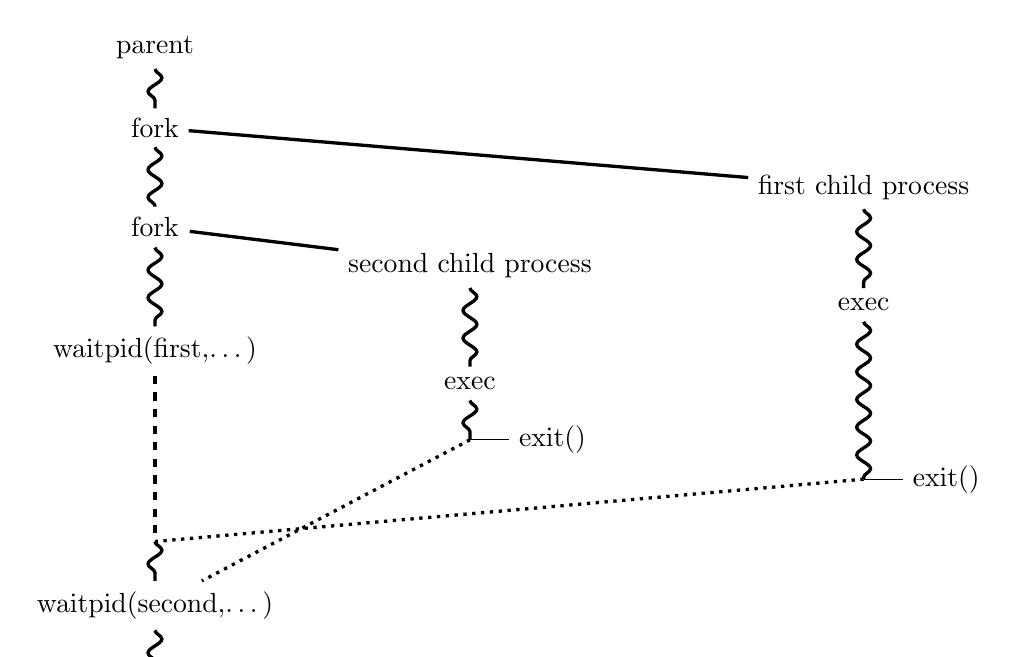
\begin{tikzpicture}
\tikzset{
    thread/.style={very thick,draw,decorate,decoration=snake},
    split/.style={very thick,draw},
    marker/.style={thin,draw},
}
\path[thread] (0, 0) --  (0, -.5);
\node[anchor=south] at (0,0) {parent};
\node[anchor=north] (fork mark 1) at (0, -.5) {fork};
\draw[thread] (fork mark 1) -- ++(0, -1) node[below] (fork mark 2) {fork};
\draw[thread] (fork mark 2.south) -- ++(0, -1) node[below] (wait 1 start) {waitpid(first,\ldots)};
\node (child 1 start) at (9, -1.5) {first child process};
\node (child 2 start) at (4, -2.5) {second child process};
\path[split] (fork mark 1) --  (child 1 start);
\path[split] (fork mark 2) --  (child 2 start);
\path[thread] (child 1 start.south) -- ++(0, -1) node[below] (exec 1) {exec};
\path[thread] (exec 1.south) -- ++(0, -2) coordinate (exec 1 done);
\path[marker] (exec 1 done) -- ++(.5, 0) node[right] {exit()};
\path[thread] (child 2 start.south) -- ++(0, -1) node[below] (exec 2) {exec};
\path[thread] (exec 2.south) -- ++ (0, -0.5) coordinate (exec 2 done);
\path[marker] (exec 2 done) -- ++(.5, 0) node[right] {exit()};
\path[split,dotted] (exec 1 done) -- (0, -6) coordinate (wait 1 done);;
\draw[very thick,dashed] (wait 1 start) -- (wait 1 done);
\draw[thread] (wait 1 done) -- ++(0, -.5) node[below] (wait 2 start) { waitpid(second,\ldots) };
\path[split,dotted] (exec 2 done) -- (wait 2 start);
\draw[overlay,thread] (wait 2 start.south) -- ++ (0, -2);
\end{tikzpicture}
\end{frame}



\subsection{POSIX and Unix}

\usetikzlibrary{calc}

\begin{frame}{this class: focus on Unix}
    \begin{itemize}
    \item Unix-like OSes will be our focus
    \item we have source code
    \item used to from 2150, etc.?
    \item have been around for a while
    \item xv6 imitates Unix
    \end{itemize}
\end{frame}

\begin{frame}{Unix history}
\vspace{-.5cm}
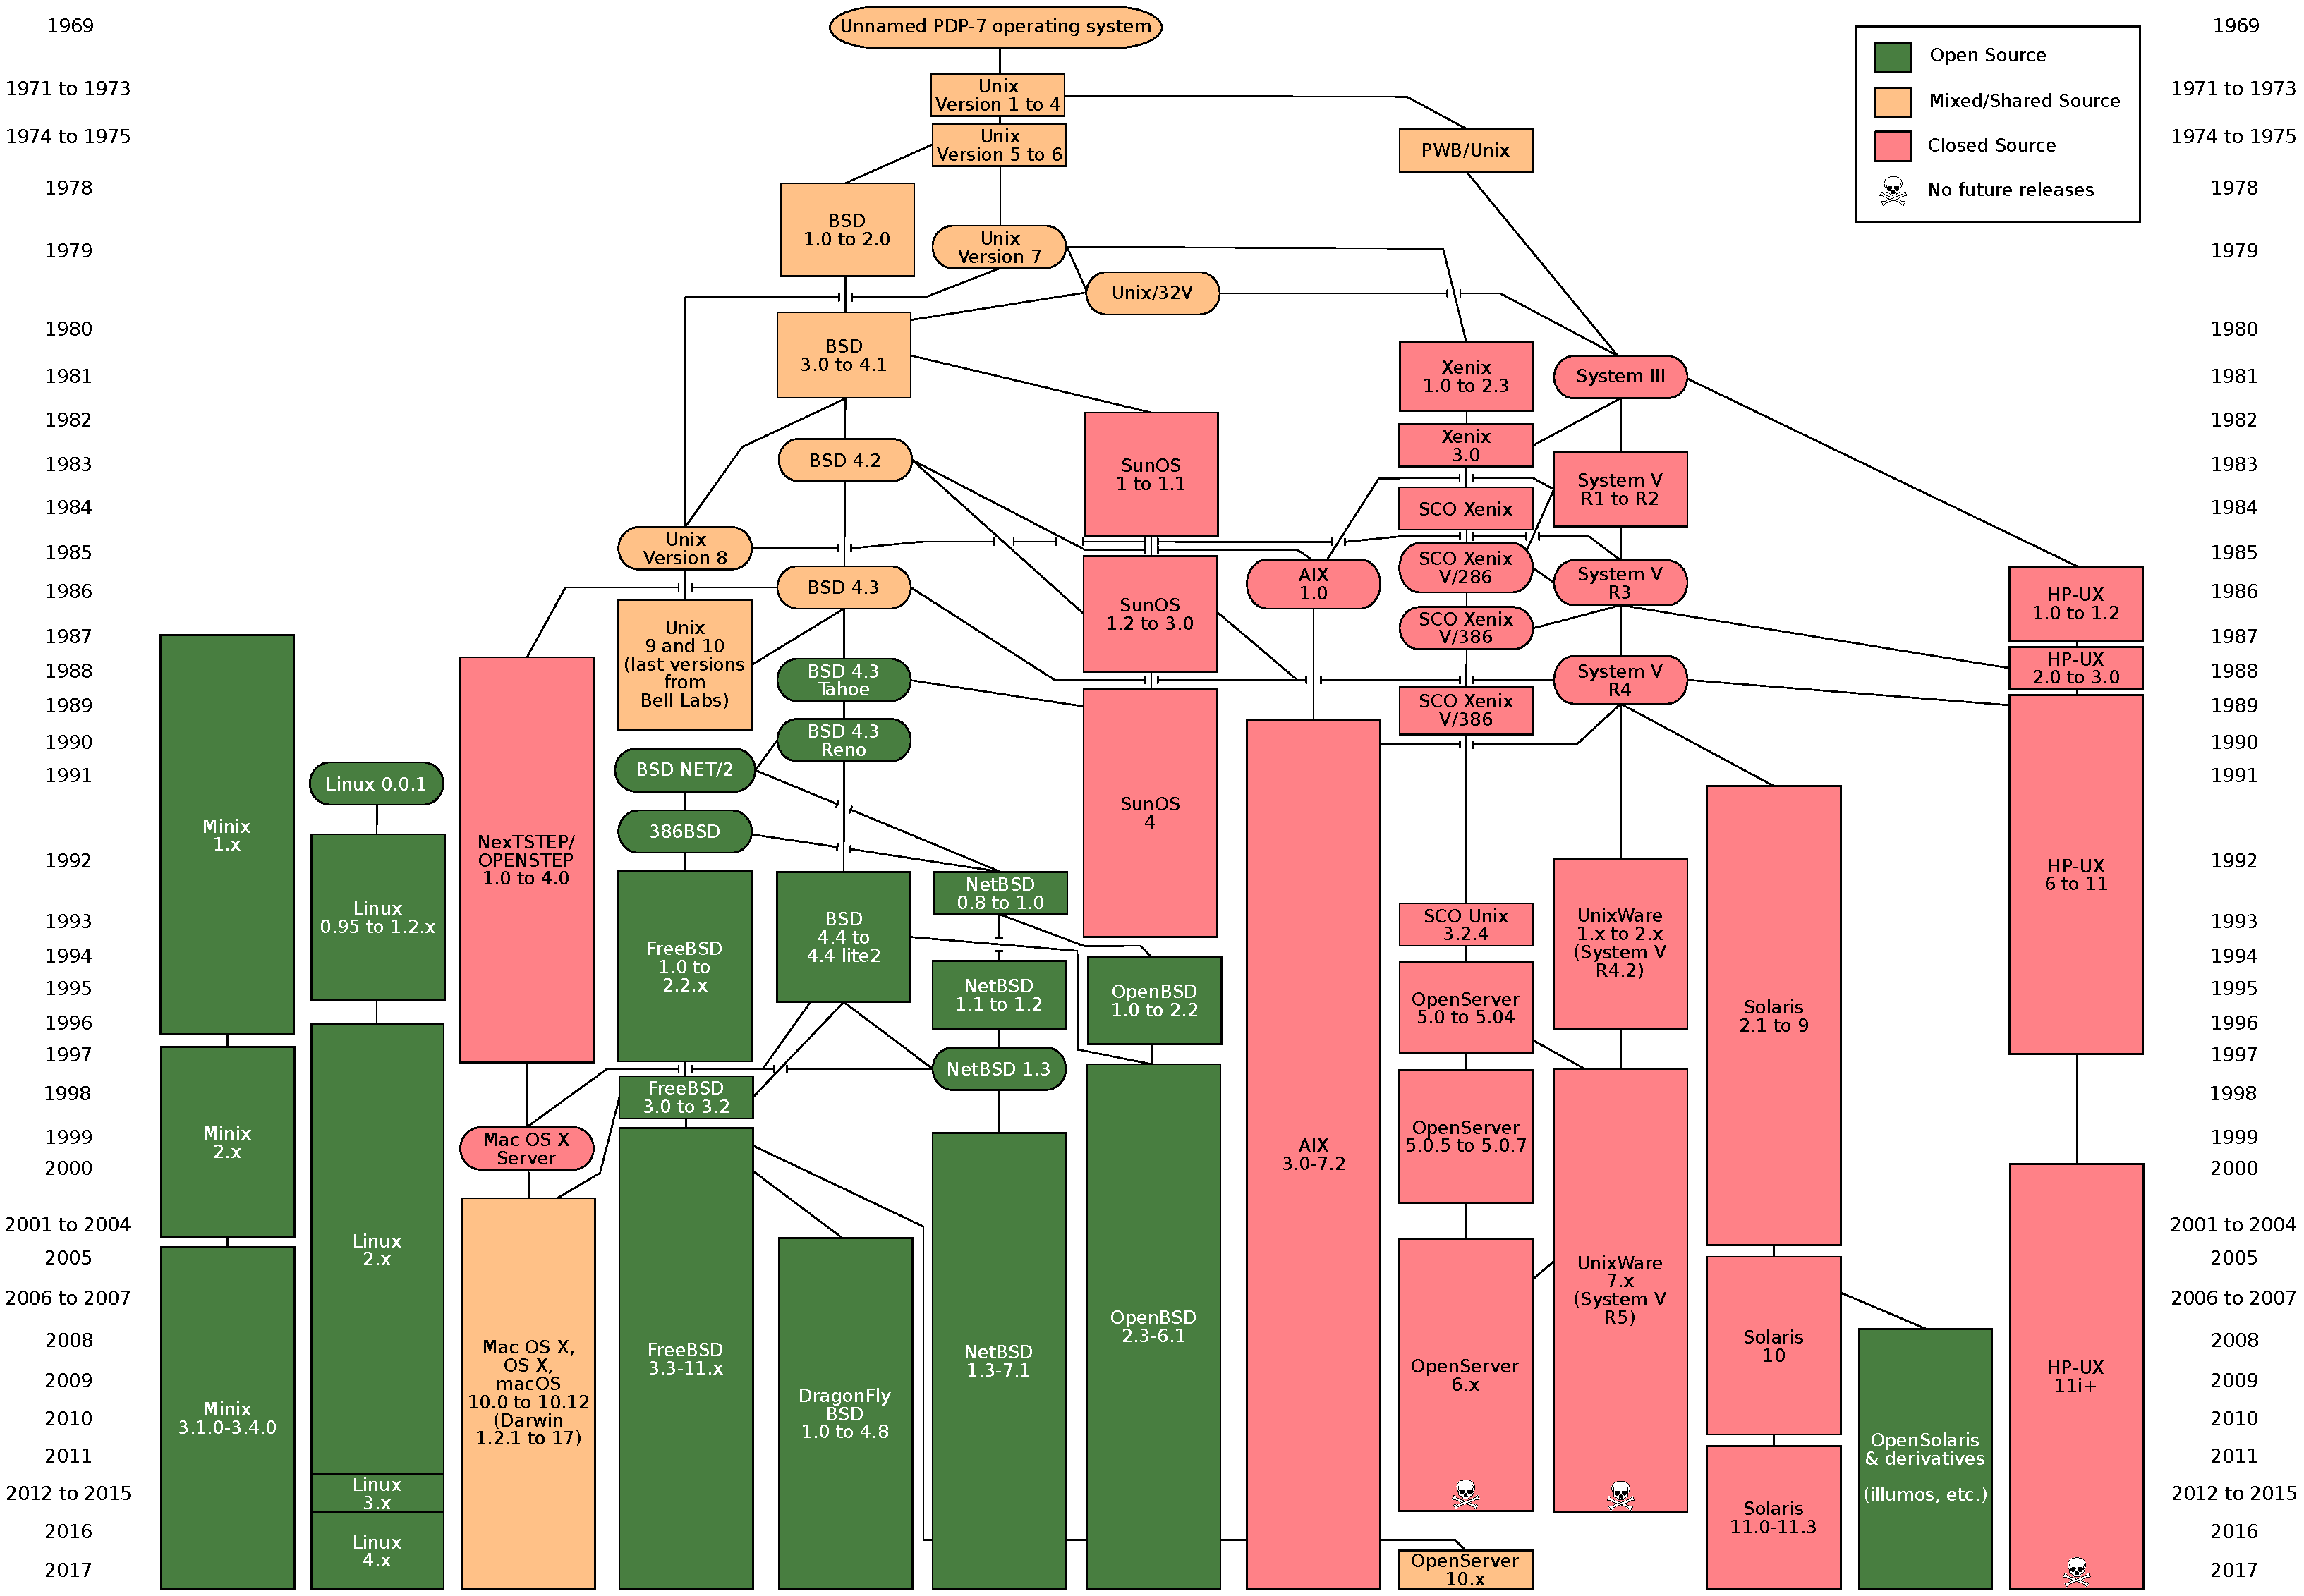
\includegraphics[height=0.9\textheight]{../unix-api/Unix_history-simple_en.pdf}
\imagecredit{image: Wikpedia/Eraserhead1+Infinity0+Sav\_vas}
\end{frame}

\begin{frame}{POSIX: standardized Unix}
\begin{itemize}
\item Portable Operating System Interface (POSIX) 
    \begin{itemize}
    \item ``standard for Unix''
    \end{itemize}
\item current version online: https://pubs.opengroup.org/onlinepubs/9699919799/
\item (almost) followed by most current Unix-like OSes
\item \ldots but OSes add extra features
\item \ldots and POSIX doesn't specify everything
\end{itemize}
\end{frame}

\begin{frame}{what POSIX defines}
\begin{itemize}
\item POSIX specifies the \myemph{library and shell interface}
    \begin{itemize}
    \item source code compatibility
    \end{itemize}
\item doesn't care what is/is not a system call\ldots
\item doesn't specify binary formats\ldots
\item idea: write applications for POSIX, recompile and run on all implementations
    \begin{itemize}
    \item this was a very important goal in the 80s/90s
    \item at the time, no dominant Unix-like OS (Linux was very immature)
    \end{itemize}
\end{itemize}
\end{frame}


\subsection{getpid}

\begin{frame}[fragile,label=getpid]{getpid}
\begin{lstlisting}[language=C++]
pid_t my_pid = getpid();
printf("my pid is %ld\n", (long) my_pid);
\end{lstlisting}
\end{frame}

\begin{frame}[fragile,label=ps]{process ids in ps}
\begin{Verbatim}
cr4bd@machine:~$ ps
  PID TTY          TIME CMD
14777 pts/3    00:00:00 bash
14798 pts/3    00:00:00 ps
\end{Verbatim}
\end{frame}


\subsection{read, write}

% FIXME: work through examples more


\begin{frame}<0>[fragile,label=readWrite]{read/write}
\begin{lstlisting}
ssize_t read(int fd, void *buffer, size_t count);
ssize_t write(int fd, void *buffer, size_t count);
\end{lstlisting}
\begin{itemize}
\item read/write \myemph<2>{up to \textit{count}} bytes to/from \textit{buffer}
\item returns number of bytes read/written or -1 on error
    \begin{itemize}
    \item ssize\_t is a signed integer type
    \item error code in \texttt{errno}
    \end{itemize}
\item read returning 0 means end-of-file (\textit{not an error})
\begin{itemize}
\item can read/write less than requested (end of file, broken I/O device, \ldots)
\end{itemize}
\end{itemize}
\end{frame}

\againframe<1>{readWrite}

\begin{frame}[fragile,label=readExample1]{read'ing one byte at a time}
\begin{lstlisting}[language=C++,style=small,morekeywords=ssize\_t,morekeywords=string]
string s;
ssize_t amount_read;
char c;
/* cast to void * not needed in C */
while ((amount_read = read(STDIN_FILENO, (void*) &c, 1)) > 0) {
    /* amount_read must be exactly 1 */
    s += c;
}
if (amount_read == -1) {
    /* some error happened */
    perror("read"); /* print out a message about it */
} else if (amount_read == 0) {
    /* reached end of file */
}
\end{lstlisting}
\end{frame}



\begin{frame}[fragile,label=writeExample]{write example}
\begin{lstlisting}[language=C++,style=small]
/* cast to void * optional in C */
write(STDOUT_FILENO, (void *) "Hello, World!\n", 14);
\end{lstlisting}
\end{frame}





\subsection{aside: environment variables}

\begin{frame}[fragile,label=envVarsPrintenv]{aside: environment variables (1)}
\begin{itemize}
\item key=value pairs associated with every process:
\end{itemize}
\begin{Verbatim}[fontsize=\fontsize{8}{9}\selectfont,commandchars=\\\{\}]
$ \textbf{printenv}
MODULE_VERSION_STACK=3.2.10
MANPATH=:/opt/puppetlabs/puppet/share/man
XDG_SESSION_ID=754
HOSTNAME=labsrv01 
SELINUX_ROLE_REQUESTED=
TERM=screen
SHELL=/bin/bash 
HISTSIZE=1000 
SSH_CLIENT=128.143.67.91 58432 22 
SELINUX_USE_CURRENT_RANGE=
QTDIR=/usr/lib64/qt-3.3
OLDPWD=/zf14/cr4bd
QTINC=/usr/lib64/qt-3.3/include
SSH_TTY=/dev/pts/0
QT_GRAPHICSSYSTEM_CHECKED=1
USER=cr4bd
LS_COLORS=rs=0:di=01;34:ln=01;36:mh=00:pi=40;33:so=01;35:do=01;35:bd=40;33;01:cd=40;33;01:or=40;31;01:mi=01;05;37;41:su=37;41:sg=30;43:ca=30;41:tw=30;42:ow=34;42:st=37;44:ex=01;32:*.tar=01;31:*.tgz=01;31:*.arc=01;31:*.arj=01;31:*.taz=01;31:*.lha=01;31:*.lz4=01;31:*.lzh=01;31:*.lzma=01;31:*.tlz=01;31:*.txz=01;31:*.tzo=01;31:*.t7z=01;31:*.zip=01;31:*.z=01;31:*.Z=01;31:*.dz=01;31:*.gz=01;31:*.lrz=01;31:*.lz=01;31:*.lzo=01;31:*.xz=01;31:*.bz2=01;31:*.bz=01;31:*.tbz=01;31:*.tbz2=01;31:*.tz=01;31:*.deb=01;31:*.rpm=01;31:*.jar=01;31:*.war=01;31:*.ear=01;31:*.sar=01;31:*.rar=01;31:*.alz=01;31:*.ace=01;31:*.zoo=01;31:*.cpio=01;31:*.7z=01;31:*.rz=01;31:*.cab=01;31:*.jpg=01;35:*.jpeg=01;35:*.gif=01;35:*.bmp=01;35:*.pbm=01;35:*.pgm=01;35:*.ppm=01;35:*.tga=01;35:*.xbm=01;35:*.xpm=01;35:*.tif=01;35:*.tiff=01;35:*.png=01;35:*.svg=01;35:*.svgz=01;35:*.mng=01;35:*.pcx=01;35:*.mov=01;35:*.mpg=01;35:*.mpeg=01;35:*.m2v=01;35:*.mkv=01;35:*.webm=01;35:*.ogm=01;35:*.mp4=01;35:*.m4v=01;35:*.mp4v=01;35:*.vob=01;35:*.qt=01;35:*.nuv=01;35:*.wmv=01;35:*.asf=01;35:*.rm=01;35:*.rmvb=01;35:*.flc=01;35:*.avi=01;35:*.fli=01;35:*.flv=01;35:*.gl=01;35:*.dl=01;35:*.xcf=01;35:*.xwd=01;35:*.yuv=01;35:*.cgm=01;35:*.emf=01;35:*.axv=01;35:*.anx=01;35:*.ogv=01;35:*.ogx=01;35:*.aac=01;36:*.au=01;36:*.flac=01;36:*.mid=01;36:*.midi=01;36:*.mka=01;36:*.mp3=01;36:*.mpc=01;36:*.ogg=01;36:*.ra=01;36:*.wav=01;36:*.axa=01;36:*.oga=01;36:*.spx=01;36:*.xspf=01;36:
MODULE_VERSION=3.2.10
MAIL=/var/spool/mail/cr4bd
PATH=/zf14/cr4bd/.cargo/bin:/zf14/cr4bd/bin:/usr/lib64/qt-3.3/bin:/usr/local/bin:/usr/bin:/usr/local/sbin:/usr/sbin:/opt/puppetlabs/bin:/usr/cs/contrib/bin:.
PWD=/zf14/cr4bd
LANG=en_US.UTF-8
MODULEPATH=/sw/centos/Modules/modulefiles:/sw/linux-any/Modules/modulefiles
LOADEDMODULES=
KDEDIRS=/usr
\textbf{\ldots}
_=/usr/bin/printenv
\end{Verbatim}
\end{frame}

\begin{frame}[fragile,label=envVarsFuncs]{aside: environment variables (2)}
\begin{itemize}
\item environment variable library functions:
    \begin{itemize}
    \item \texttt{getenv("KEY")} $\rightarrow$ \textit{value}
    \item \texttt{putenv("KEY=\textit{value}")} (sets KEY to \textit{value})
    \item \texttt{setenv("KEY", "value")} (sets KEY to \textit{value})
    \end{itemize}
\item {\fontsize{12}{13}\texttt{int execve(char *path, char **argv, char **envp)}}
\begin{lstlisting}[language=C++,style=small]
    char *envp[] = { "KEY1=value1", "KEY2=value2", NULL };
    char *argv[] = { "somecommand", "some arg", NULL };
    execve("/path/to/somecommand", argv, envp);
\end{lstlisting}
\item normal exec versions --- keep same environment variables
\end{itemize}
\end{frame}

\begin{frame}[fragile,label=envVarsUse]{aside: environment variables (3)}
\begin{itemize}
\item interpretation up to programs, but common ones\ldots
\vspace{.5cm}
\item \texttt{PATH=/bin:/usr/bin} 
    \begin{itemize}
    \item to run a program `foo', look for an executable in \texttt{/bin/foo}, then \texttt{/usr/bin/foo}
    \end{itemize}
\item \texttt{HOME=/zf14/cr4bd} 
    \begin{itemize}
    \item current user's home directory is `/zf14/cr4bd'
    \end{itemize}
\item \texttt{TERM=screen-256color} 
    \begin{itemize}
    \item your output goes to a `screen-256color'-style terminal
    \end{itemize}
\item \ldots
\end{itemize}
\end{frame}


\subsection{wait for mutliple}

\begin{frame}[fragile,label=typicalPatternMultiple1]{multiple processes?}
\begin{lstlisting}[language=C++,style=small]
while (...) {
    pid = fork();
    if (pid == 0) {
        exec ...
    } else if (pid > 0) {
        pids.push_back(pid);
    }
}

/* retrieve exit statuses in order */
for (pid_t pid : pids) {
    waitpid(pid, ...); 
    ...
}
\end{lstlisting}
\end{frame}
 

\subsection{wait for all}

\begin{frame}[fragile,label=waitForAny]{waiting for all children}
\begin{lstlisting}[
    language=C++,
    style=smaller,
    moredelim={**[is][\btHL<2|handout:0>]{@2}{2@}},
]
#include <sys/wait.h>
...
  while (true) {
    pid_t child_pid = waitpid(-1, &status, 0);
    if (child_pid == (pid_t) -1) {
      if (errno == ECHILD) {
        /* no child process to wait for */
        break;
      } else {
        /* some other error */
      }
    }
    /* handle child_pid exiting */
  }
\end{lstlisting}
\end{frame}


\subsection{wait for all (alt)}


\begin{frame}[fragile,label=typicalPatternMultiple2]{multiple processes?}
\begin{lstlisting}[language=C++,style=small]
while (...) {
    pid = fork();
    if (pid == 0) {
        exec ...
    } else if (pid > 0) {
        pids.push_back(pid);
    }
}

/* retrieve exit statuses as processes finish */
while ((pid = waitpid(-1, ...)) != -1) {
    handleProcessFinishing(pid);
}
\end{lstlisting}
\end{frame}



\subsection{waitpid WNOHANG}


\begin{frame}[fragile,label=waitNoHang]{`waiting' without waiting}
\begin{lstlisting}[
    language=C++,
    style=smaller,
    moredelim={**[is][\btHL<2|handout:0>]{@2}{2@}},
]
#include <sys/wait.h>
...
  pid_t return_value = waitpid(child_pid, &status, WNOHANG);
  if (return_value == (pid_t) 0) {
    /* child process not done yet */
  } else if (child_pid == (pid_t) -1) {
    /* error */
  } else {
    /* handle child_pid exiting */
  }
\end{lstlisting}
\end{frame}


\subsection{parent and child}

\begin{frame}{parent and child processes}
\begin{itemize}
    \item every process (but process id 1) has a \textit{parent process} (\texttt{getppid()})
    \item this is the process that can wait for it
    \item creates tree of processes (Linux \texttt{pstree} command):
\end{itemize}
    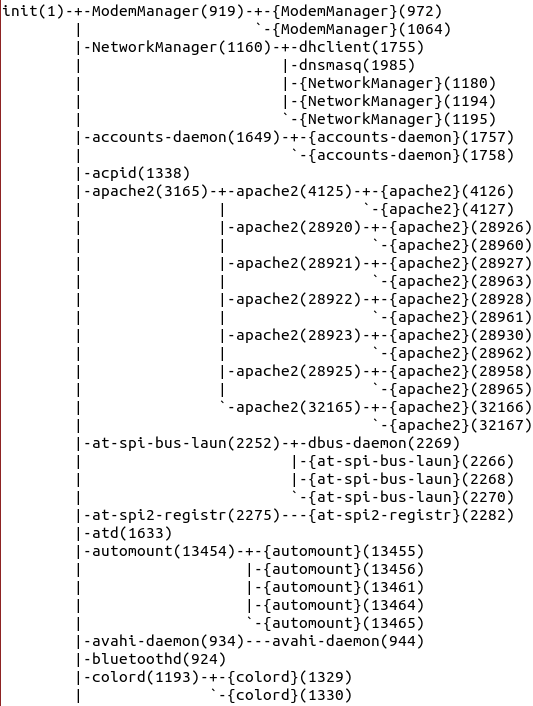
\includegraphics[height=0.6\textheight]{../unix-api/process-tree}
    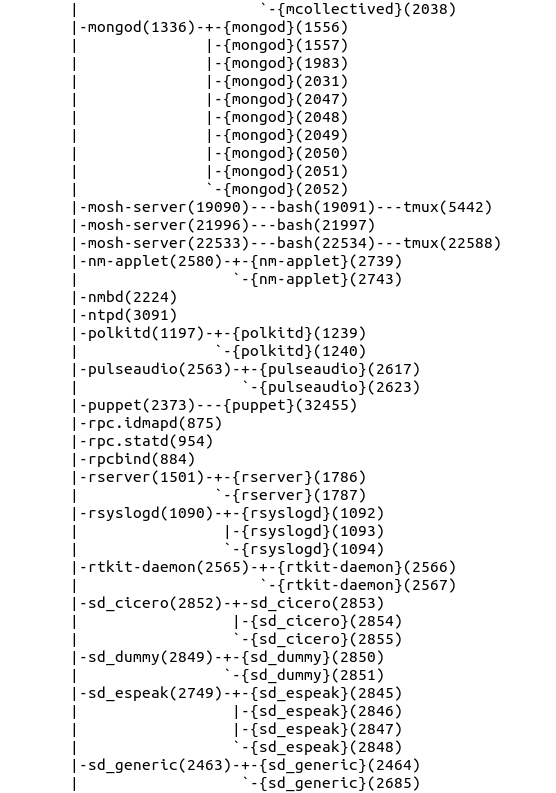
\includegraphics[height=0.6\textheight]{../unix-api/process-tree2}
\end{frame}

\begin{frame}{parent and child questions\ldots}
\begin{itemize}
    \item what if parent process exits before child?
        \begin{itemize}
        \item child's parent process becomes process id 1 (typically called \textit{init})
        \end{itemize}
    \item what if parent process never \texttt{waitpid()}s {\small (or equivalent)} for child?
        \begin{itemize}
        \item child process stays around as a ``zombie'' 
        \item can't reuse pid in case parent wants to use \texttt{waitpid()}
        \end{itemize}
    \item what if non-parent tries to \texttt{waitpid()} for child?
        \begin{itemize}
        \item waitpid fails
        \end{itemize}
\end{itemize}
\end{frame}



\subsection{exercise (read/write/dup2)}

\begin{frame}[fragile,label=ex]{exercise}
\begin{lstlisting}[style=small]
int fd = open("output.txt", O_WRONLY|O_CREAT|O_TRUNC, 0666);
write(fd, "A", 1);
dup2(STDOUT_FILENO, 100);
dup2(fd, STDOUT_FILENO);
write(STDOUT_FILENO, "B", 1);
write(fd, "C", 1);
close(fd);
write(STDOUT_FILENO, "D", 1);
write(100, "E", 1);
\end{lstlisting}
\small Assume \texttt{open()} and \texttt{dup2()} \textit{do not fail},
\texttt{write()} does not fail as long as the fd it writes to is open,
fd \texttt{100} was closed and is not what open returns, and \texttt{STDOUT\_FILENO} is initially open.
What is written to \texttt{output.txt}? \\
\begin{tabular}{llllll}
\textbf{A.} & ABCDE & \textbf{C.} & ABC & \textbf{E.} something else \\
\textbf{B.} & ABCD & \textbf{D.} & ACD \\
\end{tabular}
\end{frame}


\section{partial reads and writes}
\subsection{partial reads and read error checking}

\begin{frame}[fragile,label=readExample2]{read'ing a fixed amount}
\begin{lstlisting}[language=C++,style=small,morekeywords=ssize\_t]
ssize_t offset = 0;
const ssize_t amount_to_read = 1024;
char result[amount_to_read];
do {
    /* cast to void * optional in C */
    ssize_t amount_read = 
        read(STDIN_FILENO,
             (void *) (result + offset),
             amount_to_read - offset);
    if (amount_read < 0) {
        perror("read"); /* print error message */
        ... /* abort??? */
    } else {
        offset += amount_read;
    }
} while (offset != amount_to_read && amount_read != 0);
\end{lstlisting}
\end{frame}

\begin{frame}{partial reads}
\begin{itemize}
    \item on regular file: read reads what you request
    \item but otherwise: usually gives you what's known to be available
        \begin{itemize}
            \item after waiting for something to be available
        \end{itemize}
    \vspace{.5cm}
    \item<2-> reading from network --- what's been received
    \item<2-> reading from keyboard --- what's been typed
\end{itemize}
\end{frame}

\subsection{partial writes and write error checking}

\begin{frame}[fragile,label=writeExampleErrorChecking]{write example (with error checking)}
\begin{lstlisting}[language=C++,style=small,morekeywords=ssize\_t]
const char *ptr = "Hello, World!\n";
ssize_t remaining = 14;
while (remaining > 0) {
    /* cast to void * optional in C */
    ssize_t amount_written = write(STDOUT_FILENO,
                                   ptr,
                                   remaining);
    if (amount_written < 0) {
        perror("write"); /* print error message */
        ... /* abort??? */
    } else {
        remaining -= amount_written;
        ptr += amount_written;
    }
}
\end{lstlisting}
\end{frame}

\begin{frame}{partial writes}
\begin{itemize}
    \item usually only happen on error or interruption
        \begin{itemize}
        \item but can request ``non-blocking''
        \item (interruption: via \textit{signal})
        \end{itemize}
    \item \textit{usually}: write \myemph{waits until it completes}
        \begin{itemize}
        \item = until remaining part fits in buffer in kernel
        \item does not mean data was sent on network, shown to user yet, etc.
        \end{itemize}
\end{itemize}
\end{frame}


\subsection{kernel buffering}

\usetikzlibrary{arrows.meta,chains,shapes}

\begin{frame}{kernel buffering (reads)}
\begin{tikzpicture}
\tikzset{
    >=Latex,
    component box/.style={draw,thick,minimum width=10cm,minimum height=1cm,align=center},
    component box big/.style={component box,minimum height=2.5cm},
    component box small/.style={component box,minimum width=4cm},
    subcomponent box/.style={draw,thick,minimum width=2cm,align=center,font=\small},
    event line/.style={draw,ultra thick},
    event box/.style={draw,thick,fill=white,inner sep=0.25mm,font=\small, align=center},
    number box A/.style={draw=blue,thick,fill=blue!10,ellipse,font=\small,inner sep=0.1mm},
    number box A alt/.style={draw=blue,thick,dotted,fill=blue!5,ellipse,font=\small,inner sep=0.1mm,
            alt=<4>{draw=red,fill=red!10}},
    number box B/.style={draw=green,thick,fill=green!10,ellipse,font=\small,inner sep=0.1mm},
}
\node[component box] (process) {program};
\node[component box big,anchor=north] (os) at ([yshift=-2cm]process.south) {operating system \\ ~ \\ ~};
\node[component box small,anchor=north east] (keyboard) at ([xshift=-.5cm,yshift=-1.5cm]os.south) {keyboard};
\node[component box small,anchor=north west] (disk) at ([xshift=.5cm,yshift=-1.5cm]os.south) {disk};
\begin{visibleenv}<2->
\draw[event line,->] (keyboard.north) -- (os.south -| keyboard.north) node[midway,event box] (kp event){keypress happens, read};
\node[number box A,anchor=east] (kp event number) at (kp event.north west) {1};
\begin{visibleenv}<4->
    \node[number box A alt,anchor=east] at ([xshift=-.5cm,yshift=.1cm]kp event number.west) {2};
    \node[font=\small,anchor=east,inner sep=0.25mm] at (kp event number.west) {or};
\end{visibleenv}
\node[anchor=south,subcomponent box] (keyboard buffer)  at (os.south -| keyboard.north) {buffer: keyboard input \\ waiting for program};
\end{visibleenv}
\begin{visibleenv}<3->
    \draw[event line,->] ([xshift=-4cm]process.south) -- ([xshift=-4cm]os.north) node[midway,event box,xshift=-1cm] (read ev) {read char \\ from terminal};
\node[number box A,anchor=east] (read ev number) at (read ev.north west) {2};
\begin{visibleenv}<4->
    \node[number box A alt,anchor=east] at ([xshift=-.5cm,yshift=.1cm]read ev number.west) {1};
    \node[font=\small,anchor=east,inner sep=0.25mm] at (read ev number.west) {or};
\end{visibleenv}
    \draw[event line,<-] ([xshift=-2cm]process.south) -- ([xshift=-2cm]os.north) node[midway,event box,xshift=-.5cm] (from buf ev) {\ldots via buffer};
\node[number box A,anchor=east] at (from buf ev.north west) {3};
\end{visibleenv}
\begin{visibleenv}<5->
\draw[event line,->] ([xshift=1cm]process.south) -- ([xshift=1cm]os.north) node[midway,event box,xshift=0cm] (read file ev)  {read char \\ from file};
\node[number box B,anchor=east] at (read file ev.north west) {1};
\end{visibleenv}
\begin{visibleenv}<6->
\draw[event line,->] (disk.north) -- (os.south -| disk.north) node[midway,event box] (xfer disk ev) {read \textit{block} of data from disk};
\node[number box B,anchor=east] at (xfer disk ev.north west) {2};
\node[anchor=south,subcomponent box] at (os.south -| disk.north) {buffer: recently read \\ data from disk};
    \draw[event line,<-] ([xshift=4cm]process.south) -- ([xshift=4cm]os.north) node[midway,event box,xshift=0cm] (from disk buffer ev) {\ldots via buffer};
\node[number box B,anchor=east] at (from disk buffer ev.north west) {3};
\end{visibleenv}
\end{tikzpicture}
\end{frame}

\begin{frame}{kernel buffering (writes)}
\begin{tikzpicture}
\tikzset{
    >=Latex,
    component box/.style={draw,thick,minimum width=10cm,minimum height=1cm,align=center},
    component box big/.style={component box,minimum height=2.25cm},
    component box small/.style={component box,minimum width=4cm},
    subcomponent box/.style={draw,thick,minimum width=2cm,align=center,font=\small},
    event line/.style={draw,ultra thick},
    event box/.style={draw,thick,fill=white,inner sep=0.25mm,font=\small, align=center},
}
\node[component box] (process) {program};
\node[component box big,anchor=north] (os) at ([yshift=-2cm]process.south) {operating system \\ ~ \\ ~};
\node[component box small,anchor=north east] (network) at ([xshift=-.5cm,yshift=-1.5cm]os.south) {network};
\node[component box small,anchor=north west] (disk) at ([xshift=.5cm,yshift=-1.5cm]os.south) {disk};
\begin{visibleenv}<3->
\draw[event line,<-] (keyboard.north) -- (os.south -| keyboard.north) node[midway,event box] {(when ready) \\ send data};
\node[anchor=south,subcomponent box] (keyboard buffer)  at (os.south -| keyboard.north) {buffer: output \\ waiting for network};
\end{visibleenv}
\begin{visibleenv}<2->
\draw[event line,->] ([xshift=-4cm]process.south) -- ([xshift=-4cm]os.north) node[midway,event box,xshift=0cm] {print char \\ to remote machine};
\end{visibleenv}
\begin{visibleenv}<4->
\draw[event line,->] ([xshift=1cm]process.south) -- ([xshift=1cm]os.north) node[midway,event box,xshift=0cm] {write char \\ to file};
\end{visibleenv}
\begin{visibleenv}<5->
\draw[event line,<-] (disk.north) -- (os.south -| disk.north) node[midway,event box] {(when ready) \\ write \textit{block} of data from disk};
\node[anchor=south,subcomponent box] at (os.south -| disk.north) {buffer: data waiting \\ to be written on disk};
\end{visibleenv}
\end{tikzpicture}
\end{frame}

\begin{frame}{read/write operations}
\begin{itemize}
\item read()/write(): move data into/out of buffer
\item possibly wait if buffer is empty (read)/full (write)
\vspace{.5cm}
\item actual I/O operations --- wait for device to be ready
    \begin{itemize}
    \item trigger process to stop waiting if needed
    \end{itemize}
\end{itemize}
\end{frame}


\subsection{open}
\begin{frame}{filesystem abstraction}
\begin{itemize}
\item regular files --- named collection of bytes
    \begin{itemize}
    \item also: size, modification time, owner, access control info, \ldots
    \end{itemize}
\item directories --- folders containing files and directories
    \begin{itemize}
    \item hierarchical naming: \texttt{/net/zf14/cr4bd/fall2018/cs4414}
    \item \textit{mostly} contains regular files or directories
    \end{itemize}
\end{itemize}
\end{frame}

\begin{frame}[fragile,label=openExample]{open}
\begin{lstlisting}[
    language=C++,
    moredelim={**[is][\btHL<1-|handout:1->]{@1}{1@}},
]
int open(const char *path, int flags);
int open(const char *path, int flags, int mode);
...

int read_fd = open("dir/file1", O_RDONLY);
int write_fd = open("/other/file2",
        O_WRONLY | O_CREAT | O_TRUNC, 0666);
int rdwr_fd = open("file3", O_RDWR);
\end{lstlisting}
\end{frame}

\begin{frame}[fragile,label=openExplainPath]{open}
\begin{lstlisting}[
    language=C++,
    moredelim={**[is][\btHL<1-|handout:1->]{@1}{1@}},
]
int open(const char *@1path1@, int flags);
int open(const char *@1path1@, int flags, int mode);
\end{lstlisting}
\begin{itemize}
\item path = filename
\item e.g. \texttt{"/foo/bar/file.txt"}
    \begin{itemize}
    \item \texttt{file.txt} in 
    \item directory \texttt{bar} in
    \item directory \texttt{foo} in 
    \item ``the root directory''
    \end{itemize}
\item e.g. \texttt{"quux/other.txt}
    \begin{itemize}
    \item \texttt{other.txt} in 
    \item directory \texttt{quux} in
    \item ``the current working directory'' (set with \texttt{chdir()})
    \end{itemize}
\end{itemize}
\end{frame}

\begin{frame}[fragile,label=openExplainFDs]{open: file descriptors}
\begin{lstlisting}[
    language=C++,
    moredelim={**[is][\btHL<1-|handout:1->]{@1}{1@}},
]
@1int1@ open(const char *path, int flags);
@1int1@ open(const char *path, int flags, int mode);
\end{lstlisting}
\begin{itemize}
\item return value = \myemph{file descriptor} {\small (or -1 on error)}
\item index into table of \textit{open file descriptions} for each process
\item used by system calls that deal with open files
\end{itemize}
\end{frame}



\subsection{Unix: everything is a file}

\usetikzlibrary{arrows.meta,chains}

\begin{frame}{POSIX: everything is a file}
\begin{itemize}
\item the file: one interface for
    \begin{itemize}
    \item devices (terminals, printers, \ldots)
    \item regular files on disk
    \item networking (sockets)
    \item local interprocess communication (pipes, sockets)
    \end{itemize}
    \vspace{.5cm}
    \item basic operations: open(), read(), write(), close()
\end{itemize}
\end{frame}


\section{pipe exercise (partial reads)}

\begin{frame}<1>[fragile,label=pipeExtraEx2]{exercise}
\vspace{-.25cm}
\begin{lstlisting}[language=C++,basicstyle=\tt\fontsize{9.5}{10.5}\selectfont]
int pipe_fds[2]; pipe(pipe_fds);
pid_t p = fork();
if (p == 0) {
  close(pipe_fds[0]);
  for (int i = 0; i < 10; ++i) {
    char c = '0' + i;
    write(pipe_fds[1], &c, 1);
  }
  exit(0);
}
close(pipe_fds[1]);
char buffer[10];
ssize_t count = read(pipe_fds[0], buffer, 10);
for (int i = 0; i < count; ++i) {
  printf("%c", buffer[i]);
}
\end{lstlisting}
Which of these are possible outputs {\small (if pipe, read, write, fork don't fail)}?
\begin{tabular}{lll}
A. \texttt{0123456789} & B. \texttt{0} & C. (nothing) \\
\myemph<2>{D.} A and B & E. A and C & F. A, B, and C \\
\end{tabular}
\end{frame}

\iftoggle{heldback}{}{\againframe<2>{pipeExtraEx2}}

\begin{frame}<0>[fragile,label=pipeExtraEx2More]{empirical evidence}
\begin{Verbatim}
      8 0
    374 01
    210 012
     30 0123
     12 01234
      3 012345
      1 0123456
      2 01234567
      1 012345678
    359 0123456789
\end{Verbatim}
\end{frame}

\iftoggle{heldback}{}{\againframe<2>{pipeExtraEx2More}}

\begin{frame}{partial reads}
\begin{itemize}
\item read returning 0 always means end-of-file
    \begin{itemize}
    \item by default, read always waits \textit{if no input available yet}
    \item but can set read to return \textit{error} instead of waiting
    \end{itemize}
\item read can return less than requested if not available
    \begin{itemize}
        \item e.g. child hasn't gotten far enough
    \end{itemize}
\end{itemize}
\end{frame}
 % FIXME: cut?

\section{pipe: closing?}
\begin{frame}{pipe: closing?}
    \begin{itemize}
    \item if all write ends of pipe are closed
        \begin{itemize}
        \item can get end-of-file (read() returning 0) on read end
        \item exit()ing closes them
        \end{itemize}
    \item $\rightarrow$ close write end when not using
    \vspace{.5cm}
    \item generally: limited number of file descriptors per process
    \item $\rightarrow$ good habit to close file descriptors not being used
    \item (but probably didn't matter for read end of pipes in example)
    \end{itemize}
\end{frame}




\end{document}
